%%
%% This is file `acmmanuscript.tex',
%% generated with the docstrip utility.
%%
%% The original source files were:
%%
%% samples.dtx  (with options: `all,proceedings,manuscript')
%% 
%% IMPORTANT NOTICE:
%% 
%% For the copyright see the source file.
%% 
%% Any modified versions of this file must be renamed
%% with new filenames distinct from acmmanuscript.tex.
%% 
%% For distribution of the original source see the terms
%% for copying and modification in the file samples.dtx.
%% 
%% This generated file may be distributed as long as the
%% original source files, as listed above, are part of the
%% same distribution. (The sources need not necessarily be
%% in the same archive or directory.)
%%
%%
%% Commands for TeXCount
%TC:macro \cite [option:text,text]
%TC:macro \citep [option:text,text]
%TC:macro \citet [option:text,text]
%TC:envir table 0 1
%TC:envir table* 0 1
%TC:envir tabular [ignore] word
%TC:envir displaymath 0 word
%TC:envir math 0 word
%TC:envir comment 0 0
%%
%% The first command in your LaTeX source must be the \documentclass
%% command.
%%
%% For submission and review of your manuscript please change the
%% command to \documentclass[manuscript, screen, review]{acmart}.
%%
%% When submitting camera ready or to TAPS, please change the command
%% to \documentclass[sigconf]{acmart} or whichever template is required
%% for your publication.
%%
%%
\documentclass[manuscript,screen,review]{acmart}
%%
%% \BibTeX command to typeset BibTeX logo in the docs
\AtBeginDocument{%
  \providecommand\BibTeX{{%
    Bib\TeX}}}

%% Rights management information.  This information is sent to you
%% when you complete the rights form.  These commands have SAMPLE
%% values in them; it is your responsibility as an author to replace
%% the commands and values with those provided to you when you
%% complete the rights form.
\setcopyright{none}
\copyrightyear{2026}
\acmYear{2026}
\acmDOI{}
%% These commands are for a PROCEEDINGS abstract or paper.
%%
%%  Uncomment \acmBooktitle if the title of the proceedings is different
%%  from ``Proceedings of ...''!
%%
%%\acmBooktitle{Woodstock '18: ACM Symposium on Neural Gaze Detection,
%%  June 03--05, 2018, Woodstock, NY}
\acmJournal{TOG}


%%
%% Submission ID.
%% Use this when submitting an article to a sponsored event. You'll
%% receive a unique submission ID from the organizers
%% of the event, and this ID should be used as the parameter to this command.
%%\acmSubmissionID{123-A56-BU3}

%%
%% For managing citations, it is recommended to use bibliography
%% files in BibTeX format.
%%
%% You can then either use BibTeX with the ACM-Reference-Format style,
%% or BibLaTeX with the acmnumeric or acmauthoryear sytles, that include
%% support for advanced citation of software artefact from the
%% biblatex-software package, also separately available on CTAN.
%%
%% Look at the sample-*-biblatex.tex files for templates showcasing
%% the biblatex styles.
%%
%%
%% The majority of ACM publications use numbered citations and
%% references.  The command \citestyle{authoryear} switches to the
%% "author year" style.
%%
%% If you are preparing content for an event
%% sponsored by ACM SIGGRAPH, you must use the "author year" style of
%% citations and references.
%% Uncommenting
%% the next command will enable that style.
%%\citestyle{acmauthoryear}

\citestyle{acmauthoryear}
\usepackage{amsmath,amsfonts}
\usepackage{graphicx}
\usepackage{array}
\usepackage{tabularx}
\usepackage{multirow}
\usepackage{booktabs}
\usepackage{makecell}
\usepackage{placeins}

\newcommand{\suppvideo}{\href{https://github.com/zhjccoffee/Supplementary-supporting-video}{supplementary video}}
\newcolumntype{L}[1]{>{\raggedright\arraybackslash}m{#1}}
\newcolumntype{Y}{>{\raggedright\arraybackslash}X}


%%
%% end of the preamble, start of the body of the document source.
\begin{document}

% Paper content begins here.
\title{
Reflex-Informed Neuromuscular Reinforcement Learning for Muscle-Driven Locomotion
}
% \title{
% Low-Dimensional Residual-Reflex-Informed Deep Reinforcement Learning for Musculoskeletal Gait Generation
% }
\author{First A. Author}
\affiliation{%
  \institution{University of Leeds}
  \city{Leeds}
  \country{United Kingdom}}
\email{author@example.com}
\author{Second B. Author}
\affiliation{%
  \institution{University of Leeds}
  \city{Leeds}
  \country{United Kingdom}}
\email{author@example.com}
\author{Third C. Author}
\affiliation{%
  \institution{University of Leeds}
  \city{Leeds}
  \country{United Kingdom}}
\email{author@example.com}

\begin{abstract}
% Muscle-driven gait controllers must coordinate many actuators and remain stable
% when muscle capacity or external loading changes. Direct muscle-control deep
% reinforcement learning (DRL) can adjust its actions from the current state but
% must learn muscle coordination from task rewards, whereas optimized reflex
% controllers encode coordination but keep their parameters fixed after
% optimization. We propose Residual-Reflex RL to combine structured reflex control
% with state-dependent parameter adjustment. A five-phase reflex controller maps
% delayed muscle and posture feedback to stimulation for 18 muscle--tendon units.
% At each control step, an MPO-trained policy outputs four residual values that
% modify selected reflex gains and thresholds for hip swing, knee support, and
% ankle propulsion; the policy does not command individual muscles directly. On a
% 9-degree-of-freedom musculoskeletal character, the method achieved the smallest
% speed error and the highest average human-reference kinematic score at 0.8, 1.0,
% and 1.2~m/s among the tested controllers. The same 1.2~m/s policy completed full
% episodes with soleus strength reduced to 83\% and remained upright for 20.1~s in
% the single-100N-push test without retraining; the fixed reflex baseline
% terminated after 4.6~s in the same push test.

Muscle-driven locomotion provides a physically grounded approach to generating realistic human movement. However, achieving both physiological plausibility and adaptability to changes in musculoskeletal capacity and external disturbances remains a fundamental challenge. To address this limitation, we propose a Reflex-Informed Neuromuscular Reinforcement Learning framework for muscle-driven locomotion. Within this framework, a fixed phase-dependent reflex controller serves as the underlying neuromuscular control mechanism, while the reinforcement learning policy produces four biomechanically meaningful residual parameters to modulate key reflex gains and thresholds associated with hip swing, knee support, and ankle propulsion according to the current state. Experimental results demonstrate that the proposed framework generates physiologically plausible locomotion with improved kinematic accuracy and dynamic consistency, as well as better bilateral symmetry and stride-to-stride consistency under nominal walking conditions. The learned policy remains robust under muscle weakness and external perturbations without retraining.

\end{abstract}

\begin{CCSXML}
<ccs2012>
 <concept>
  <concept_id>10010147.10010257.10010258.10010259</concept_id>
  <concept_desc>Computing methodologies~Reinforcement learning</concept_desc>
  <concept_significance>500</concept_significance>
 </concept>
</ccs2012>
\end{CCSXML}
\ccsdesc[500]{Computing methodologies~Reinforcement learning}

\keywords{Muscle-driven locomotion, musculoskeletal simulation,
reflex-based control, residual reinforcement learning, neuromuscular control,
physics-based character animation}

\maketitle

\section{Introduction}
\label{sec:introduction}
% 第一段：Problem（不是方法）
% 随着物理驱动角色动画、数字人以及肌骨仿真的不断发展，肌肉驱动运动生成逐渐成为生成高真实性人体运动的重要研究方向。与直接指定关节轨迹或关节力矩不同，肌肉驱动模型通过神经肌肉系统、肌肉动力学和身体与环境之间的物理交互自然产生运动，因此能够生成具有更高物理一致性和生物合理性的角色动画。然而，对于一个真实的人体角色，生成的运动不仅需要具有接近人体的运动组织和动力学特征，还应能够在身体能力下降或环境发生变化时重新组织运动。因此，如何同时获得具有生理合理性的运动生成能力以及对身体和环境变化的适应能力，成为肌肉驱动角色动画中的关键挑战。
Muscle-driven simulation plays an integral role in physically based character animation and the modeling of human locomotion \cite{sun2024,schumacher2025}. Unlike approaches that directly generate motion through joint trajectories or joint torques, muscle-driven models allow movement to emerge naturally from neuromuscular control, muscle dynamics, and physical interactions between the body and the environment, resulting in motion with greater physical consistency and biological plausibility. However, realistic muscle-driven locomotion requires not only physiological plausibility, but also the ability to adapt naturally to changes in the musculoskeletal condition and the environment. Therefore, achieving both physiological plausibility and adaptability remains a key challenge in muscle-driven character animation.

% 第二段：Existing Paradigms（不是 Related Work）
% 现有肌肉驱动控制方法大致体现了两种不同的控制思想。一类方法采用反射控制、中央模式发生器（CPG）、肌肉协同等结构化神经肌肉控制模型，将部分生物运动规律直接编码到控制器中，从而能够生成稳定且具有生理意义的运动。然而，这类控制器通常依赖人工设计或离线优化，其控制规律在部署过程中保持固定，因此难以适应身体能力或环境条件的变化。另一类方法采用强化学习直接学习肌肉动作，由策略根据当前状态生成各肌肉控制信号，从而具有较强的在线适应能力。然而，由于策略需要在高维且冗余的肌肉动作空间中重新学习肌肉协调关系，仅依靠任务奖励并不能保证生成运动具有接近人体的运动组织和动力学特征。现有方法因此往往在生理合理性与适应能力之间形成取舍：结构化控制保留了生物运动组织，却缺乏状态依赖调节；直接肌肉学习具有适应能力，却需要重新发现复杂的神经肌肉协调。
Existing approaches to muscle-driven locomotion generally fall into two categories. One category employs structured neuromuscular controllers, such as reflex-based control, central pattern generators (CPGs), and muscle synergies, by explicitly embedding biological control principles into the controller. Such controllers naturally generate stable and physiologically meaningful locomotion. However, they are typically designed manually or optimized offline, and their control policies remain fixed during deployment, limiting their ability to adapt to changes in musculoskeletal conditions or the environment.
The other category formulates locomotion as a reinforcement learning problem by directly learning muscle actions. Since muscle activations are generated online according to the current state, these methods exhibit strong adaptability. However, directly learning muscle actions requires the policy to discover effective neuromuscular coordination within a high-dimensional and redundant action space. Task-level rewards specify the desired locomotion objective but do not explicitly determine how muscle activity should be organized, making it difficult to ensure physiologically plausible movement and dynamics. Consequently, existing approaches often face a trade-off between physiological plausibility and adaptability: structured neuromuscular controllers preserve biological organization but lack state-dependent adaptation, whereas direct muscle learning remains adaptive but must rediscover complex neuromuscular coordination from scratch.

% 第三段：Our Insight（全文灵魂）
% 我们认为，上述取舍不仅来自所采用的学习算法，更来自于强化学习学习对象（learning target）的选择。现有强化学习通常将肌肉动作作为策略直接学习的对象，而任务奖励决定了"完成什么任务"，却并不能唯一决定"如何协调肌肉完成任务"。因此，策略需要从任务奖励中重新学习复杂的神经肌肉协调规律。然而，从生物运动控制的角度来看，人体运动并不是通过直接控制每块肌肉产生的，而是在已有神经肌肉控制机制基础上，通过感觉反馈、脊髓调节以及肌肉动力学共同组织形成。 换言之，大量局部协调和运动组织已经编码在神经肌肉控制过程中。如果这些控制规律已经存在，那么强化学习是否仍然需要重新学习它们，还是应该建立在这些已有控制规律之上？这一问题启发我们重新思考强化学习在肌肉驱动运动中的作用：学习不再直接合成肌肉动作，而是学习如何调节已有神经肌肉控制机制。 在这种学习表述下，神经肌肉控制负责组织运动，而强化学习负责根据当前身体状态调节这些控制机制，从而在保留已有运动组织规律的同时赋予其状态依赖的适应能力。

From the perspective of biological motor control, locomotion is not generated by independently controlling individual muscles. Instead, muscle activity is organized through existing neuromuscular mechanisms involving sensory feedback, spinal regulation, and muscle dynamics. In other words, existing neuromuscular mechanisms already organize how sensory feedback regulates muscle activity during locomotion. If these control principles already exist, should reinforcement learning still rediscover them, or should it instead build upon them?
This question motivates us to rethink the role of reinforcement learning in muscle-driven locomotion. Rather than directly learning muscle actions, we formulate learning as the state-dependent regulation of existing neuromuscular control mechanisms. In this formulation, neuromuscular control is responsible for coordinating muscle activity, while reinforcement learning adjusts these control mechanisms according to the current state, enabling adaptation without relearning muscle coordination from scratch.

% ________________________________________
% 第四段：Our Method
% 基于这一思想，本文提出一种 Reflex-Informed Neuromuscular Learning 框架用于肌肉驱动运动生成，并以相位相关反射控制器作为神经肌肉控制机制的具体实现。在该框架中，强化学习策略不再直接输出18维肌肉动作，而是在每个控制时刻输出4个具有明确生物力学意义的残差，对髋部摆动、膝关节支撑和踝关节推进相关的反射增益与阈值进行状态依赖调节。固定反射控制器负责维持已有神经肌肉控制规律及运动组织，而学习策略则根据当前身体状态动态调节这些控制机制的工作方式，从而赋予控制器适应身体能力和环境变化的能力。由此，强化学习从直接学习肌肉执行转变为学习神经肌肉调节，使已有神经肌肉控制规律成为学习过程的一部分，而非需要重新学习的目标，并最终将高维肌肉动作学习重新表述为一个低维、可解释且具有生物学意义的神经肌肉调节问题。

Motivated by this insight, we propose a Reflex-Informed Neuromuscular Learning framework for muscle-driven locomotion, where a fixed phase-dependent reflex controller provides the underlying neuromuscular control mechanism. Rather than directly outputting 18-dimensional muscle actions, the reinforcement learning policy produces four biomechanically meaningful residual signals at each control step to modulate the gains and thresholds associated with hip swing, knee support, and ankle propulsion in a state-dependent manner. This provides a compact, interpretable, and biologically meaningful learning interface for muscle-driven locomotion.
% ________________________________________
% 第五段：Experiments + Contribution
% 为了验证所提出的 Reflex-Informed Neuromuscular Learning 框架是否能够同时实现生理合理性与适应能力，我们分别从这两个方面进行验证。正常步态实验通过人体参考运动学、地面反作用力、双侧对称性以及步间重复性等指标，评估生成运动是否具有接近人体的运动组织与动力学一致性；肌肉无力与外部扰动实验则分别评估策略在身体条件变化和环境变化下无需重新训练的适应能力。
% 本文的主要贡献如下：
To verify that the proposed Reflex-Informed Neuromuscular Learning framework provides both physiological plausibility and adaptability, we conduct complementary experiments under nominal walking, muscle weakness, and external perturbation conditions. Under nominal walking conditions, physiological plausibility is evaluated through human reference kinematics, ground reaction forces, bilateral symmetry, and stride-to-stride consistency. Muscle weakness and external perturbation experiments further evaluate the policy's ability to adapt to changes in musculoskeletal conditions and the environment without retraining. The main contributions of this work are summarized as follows:
\begin{enumerate}

% 1.	提出一种 Reflex-Informed Neuromuscular Learning 框架。 不同于直接学习肌肉动作，本文将强化学习重新表述为对已有神经肌肉控制机制进行状态依赖调节，并以固定相位相关反射控制器作为具体实现。
\item We propose a Reflex-Informed Neuromuscular Reinforcement Learning framework that reformulates reinforcement learning as the state-dependent regulation of existing neuromuscular control mechanisms, rather than directly learning muscle actions.
% 2.	提出一种紧凑且可解释的神经肌肉调节学习接口。 通过四个具有明确生物力学意义的残差参数，对固定反射控制器中的关键反馈通路进行状态依赖调节，而无需直接控制全部肌肉动作，从而实现低维、可解释的神经肌肉调节。
\item We introduce a compact and interpretable learning interface that modulates key pathways of a fixed reflex controller through four biomechanically meaningful residual parameters, enabling neuromuscular regulation without directly controlling individual muscles.
% 3.	系统验证所提出框架在生理合理性与适应能力上的优势。 通过正常步态、肌肉无力以及外部扰动实验，证明所提出框架能够在保持人体运动组织规律的同时，对身体和环境变化表现出良好的适应能力。
\item We demonstrate that the proposed framework improves physiological plausibility while maintaining adaptability across different locomotion conditions. Extensive experiments show more human-like joint kinematics, ground reaction forces, and gait consistency across multiple walking speeds, while the same trained policy remains effective under muscle weakness and external perturbations without retraining.

\end{enumerate}

% Muscle-driven simulation generates movement from muscle stimulation,
% muscle--tendon force, skeletal dynamics, and physical contact. It is used to
% study human movement and to develop bio-inspired character and assistive control
% systems \cite{anderson2001,geijtenbeek2013,lee2019,degroote2021,uchida2020}. A
% gait controller for these applications should both reproduce human-like walking
% and maintain walking when muscle strength or external loading changes.

% Current control formulations do not provide both properties reliably. A direct
% muscle-control DRL policy can change every muscle command from the current state,
% but it must learn coordination among redundant actuators from task rewards.
% Completing a speed-tracking task therefore does not by itself guarantee
% human-reference joint motion, contact loading, symmetry, or repeatability. A
% reflex controller instead specifies sparse, phase-dependent feedback pathways
% that coordinate muscles. This structure can generate stable nominal gait, but
% its gains and thresholds are normally fixed after offline optimization and
% cannot be adjusted to a weakened muscle model or a new external load. The
% specific problem addressed in this work is to retain the coordination structure
% of reflex control while allowing the controller to adjust it online.

% We propose Residual-Reflex RL for this purpose. The low-level controller uses a
% five-phase reflex topology to convert delayed muscle length, velocity, force,
% and posture feedback into muscle stimulation. The learned policy does not output
% 18 muscle stimulations. Instead, at every control step it outputs residual
% changes to four selected reflex gains and thresholds that control hip swing,
% knee support, and ankle propulsion. The fixed reflex topology supplies the
% coordination prior, and the four state-dependent residuals provide the online
% adjustment.

% We compare the method with direct muscle-control policies and a fixed
% CMA-ES-optimized reflex controller. Nominal experiments test speed tracking,
% joint kinematics, ground-reaction forces, symmetry, and cycle repeatability at
% 0.8, 1.0, and 1.2~m/s. Additional experiments apply the same trained 1.2~m/s
% policy to reduced soleus strength and backward torso pushes without retraining.

% This study makes three main contributions.
% \begin{enumerate}
%     \item We combine a fixed phase-dependent reflex topology with a learned
%     policy that adjusts reflex parameters from the current musculoskeletal state.
%     Learning changes the feedback controller instead of replacing it with direct
%     muscle commands.
%     \item We define a four-dimensional action space for selected hip-, knee-,
%     and ankle-related reflex gains and thresholds. This replaces 18 direct muscle
%     actions with four named control channels whose effects remain dependent on
%     gait phase and sensory feedback.
%     \item We evaluate nominal gait and adaptation separately. The nominal tests
%     compare speed, joint kinematics, ground-reaction forces, symmetry, and
%     repeatability at three speeds. The adaptation tests keep the trained policy
%     fixed while changing soleus strength and applying backward torso pushes.
% \end{enumerate}

% The remainder of the paper reviews related work, presents the residual-reflex
% formulation, and evaluates the learned controller in nominal walking,
% plantarflexor weakness, and external push perturbations.

\section{Related Work}
\label{sec:related-work}

\subsection{Muscle-Driven Character Simulation}
Musculoskeletal models driven by muscle–tendon dynamics have become a standard framework for studying and generating human locomotion by explicitly modeling muscle activation, muscle–tendon dynamics, skeletal dynamics, and body–environment interaction. In biomechanics, these models have been widely used to generate and analyze healthy and pathological gait, investigate locomotor strategies, study energetic objectives, and evaluate the effects of ageing and musculoskeletal impairments \cite{anderson2001,ackermann2010,falisse2019,song2018,degroote2021,uchida2020,ezati2019,dembia2020}. In computer graphics, muscle-driven simulation has been adopted for physically based character animation, enabling realistic locomotion through muscle-actuated simulation and control \cite{wang2010,wang2012,geijtenbeek2013,lee2019}. Together, these studies establish muscle-driven simulation as a mature foundation for generating realistic human locomotion. Consequently, recent research has increasingly focused on how to design effective controllers for these musculoskeletal systems.

% In computer graphics, Wang et al. optimized walking controllers for uncertain inputs and environments [2010] and used biologically based actuators and objectives for locomotion control [2012]. Geijtenbeek et al. developed flexible muscle-based locomotion for bipedal creatures [2013], and Lee et al. introduced a scalable framework for muscle-actuated human simulation and control [2019]. These studies establish muscle-driven simulation as a practical foundation for biomechanical analysis and physically based character animation. The central question for the present work is therefore not how to construct a musculoskeletal character, but how to control its muscles. The following sections review structured neuromuscular controllers and learning-based muscle control.


% Physics-based muscle-driven simulation connects control decisions to internal
% muscle loading and mechanically consistent character motion. In biomechanics,
% dynamic optimization and predictive simulation use musculoskeletal dynamics
% and task objectives to generate gait without prescribing the complete motion.
% They have been used to study healthy and pathological walking, energetic
% objectives, ageing, and the effects of model or task constraints
% \cite{anderson2001,ackermann2010,falisse2019,song2018,degroote2021}. Direct
% collocation and musculoskeletal optimal-control software have made these
% trajectory-level problems increasingly tractable \cite{falisse2019,dembia2020}.



% Graphics research has pursued a complementary goal by optimizing feedback
% controllers for uncertain environments and by incorporating biologically based
% actuators into character locomotion \cite{wang2010,wang2012}. Subsequent systems
% have improved the flexibility and scalability of muscle-actuated character
% simulation and control \cite{geijtenbeek2013,lee2019}. Together, these studies
% show that muscle and contact dynamics can produce plausible character motion,
% but they do not all provide the same form of adaptation. A trajectory optimized
% for one model and task is not itself a feedback policy. An optimized feedback
% controller can react within its designed operating regime, yet its coordination
% parameters generally remain fixed after optimization and need not accommodate
% unseen changes in muscle capacity or external loading.

\subsection{Structured Neuromuscular Control}
Biologically inspired controllers introduce prior knowledge of human motor control directly into the control architecture. Representative approaches include central pattern generators (CPGs), muscle synergies, and reflex-based controllers. Ijspeert reviewed CPG-based locomotion control in animals and robots, where rhythmic movement is generated through coupled oscillatory networks \cite{ijspeert2008}. d'Avella et al. and Meyer et al. modeled muscle coordination using muscle synergies, representing muscle activation with a reduced set of coordinated control signals \cite{davella2003,meyer2016}. Geyer and Herr proposed a reflex-based controller that generates human walking through physiologically motivated sensory feedback \cite{geyer2010}, which was later extended by Song and Geyer to generate diverse locomotion behaviors across different walking speeds \cite{song2015}. Dzeladini et al. further combined CPGs and reflexes within a unified neuromuscular controller \cite{dzeladini2014}.

Among these approaches, reflex-based control is particularly relevant to muscle-driven locomotion because it directly maps muscle sensory feedback to muscle stimulation. Reflex-based controllers have been shown to generate stable locomotion in humans \cite{geyer2010,song2015}, adaptive walking across a wide range of speeds \cite{koseki2024}, and robust locomotion in bipedal robots \cite{batts2015}. However, most existing reflex controllers rely on manually designed or offline-optimized parameters. Although muscle stimulation changes continuously with sensory feedback, the underlying reflex gains and thresholds are not updated online, limiting adaptation to changes in musculoskeletal conditions and the environment.
\subsection{Learning-Based Muscle Control}
Deep reinforcement learning has enabled physics-based characters to acquire locomotion skills directly through interaction with the environment, while prior work has shown that the action representation and reference-motion objective strongly affect the learned behavior \cite{peng2017,peng2018}. For muscle-driven characters, existing approaches typically formulate muscle activations as the policy output, allowing muscle control signals to be generated online according to the current state \cite{weng2021,devree2021,ogum2024,song2021}. Compared with manually designed controllers, these methods improve adaptability and can learn complex locomotion behaviors without explicitly specifying muscle coordination.

Recent studies have further improved direct muscle-control reinforcement learning from different perspectives. Bio-inspired reward functions encourage more physiologically realistic gait patterns \cite{nowakowski2021,schumacher2025}. Model-based reinforcement learning incorporates musculoskeletal dynamics into policy optimization
\cite{su2023}. DEP-RL improves exploration in overactuated musculoskeletal systems through embodied exploratory feedback \cite{deprl2023}. More recently, AI-CPG combines a CPG-based feedforward controller with a learned reflex network to improve adaptive locomotion \cite{li2024}.

Overall, these studies indicate that existing approaches cannot simultaneously provide physiological plausibility and adaptability. Structured neuromuscular controllers can generate physiologically plausible movement but struggle to adapt to changes in the musculoskeletal model or the environment, whereas reinforcement learning-based muscle control improves adaptation in muscle-driven locomotion but often generates gait patterns that deviate from human kinematics and dynamics.




\section{Method}
\label{sec:method}
\subsection{Framework Overview}
Figure~\ref{framwork} illustrates the proposed Reflex-Informed Neuromuscular Reinforcement Learning framework. A fixed phase-dependent reflex controller provides the underlying neuromuscular control mechanism, while the reinforcement learning policy generates four-dimensional residual actions that regulate selected reflex parameters according to the current musculoskeletal state. The resulting muscle stimulation drives the musculoskeletal simulation, which produces the next state and reward. During learning, transitions $(\mathbf{s}_t,\mathbf{a}_t,r_t,\mathbf{s}_{t+1})$
are stored in the replay buffer $\mathcal{D}$. Maximum a Posteriori Policy Optimization (MPO) updates the policy through an off-policy actor–critic framework using replayed transitions \cite{mpo2018}.

% Figure~\ref{framwork} shows the execution loop and the learning loop. During
% execution, the policy maps the current musculoskeletal state $\mathbf{s}_t$ to a
% four-dimensional residual action $\mathbf{a}_t$. These four values modify four
% parameters of the phase-dependent reflex controller. The controller then maps
% delayed muscle and posture feedback to muscle stimulation, and the
% musculoskeletal simulation produces the next state $\mathbf{s}_{t+1}$ and
% reward. The reflex topology and muscle model remain fixed; only the four
% selected reflex parameters are adjusted online.

% During learning, transitions $(\mathbf{s}_t,\mathbf{a}_t,r_t,\mathbf{s}_{t+1})$
% are stored in the replay buffer $\mathcal{D}$. A critic
% $q(\mathbf{s},\mathbf{a};\boldsymbol{\omega})$ evaluates actions, and Maximum a
% Posteriori Policy Optimization (MPO) updates the rollout policy
% \cite{mpo2018}. Panels (b1) and (b2) in Fig.~\ref{framwork} show the
% phase-dependent reflex pathways and fixed proprioceptive feedback loop,
% respectively. The following sections define each part of this computation.

\begin{figure*}[!t]
\centerline{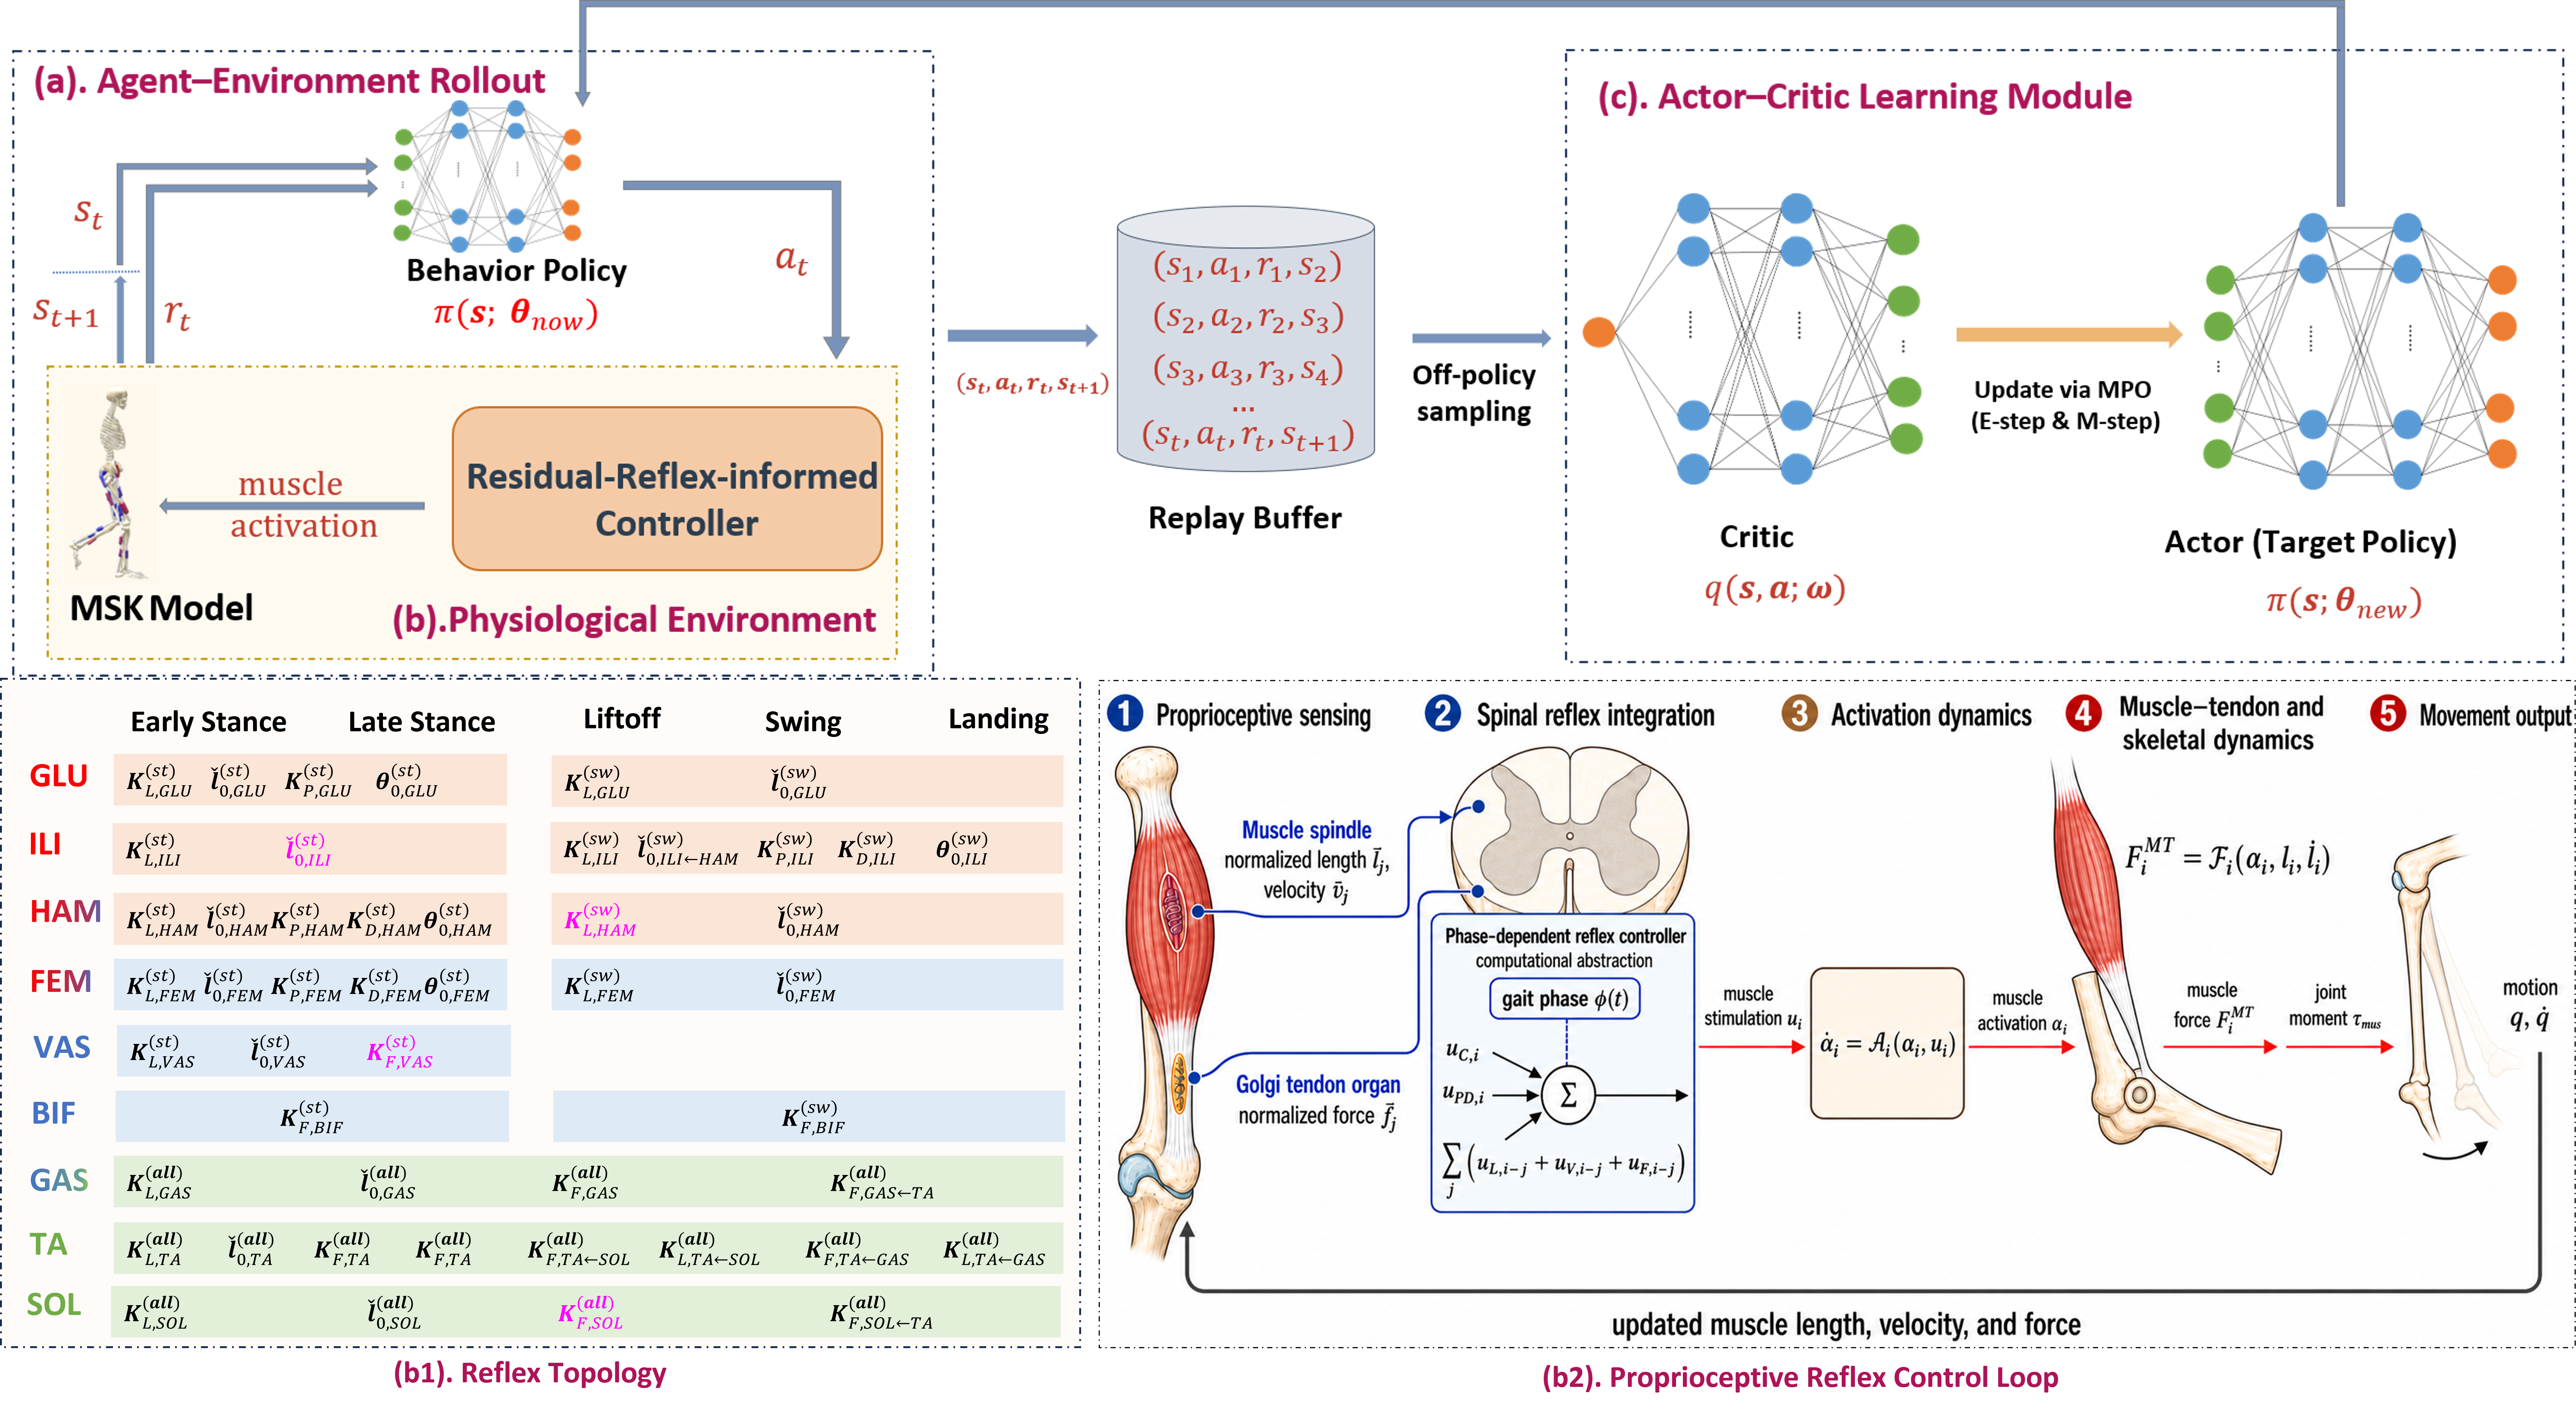
\includegraphics[width=\textwidth]{framwork1.png}}
\caption{Overview of the proposed Residual-Reflex RL framework. (a) The
rollout policy maps the musculoskeletal state $\mathbf{s}_t$ to a
four-dimensional residual action $\mathbf{a}_t$ and collects transitions
$(\mathbf{s}_t,\mathbf{a}_t,r_t,\mathbf{s}_{t+1})$. (b) The physiological
environment combines the muscle-driven character with a phase-dependent
residual-reflex-informed controller. In the enlarged lower row, panel (b1) on
the left shows the sparse phase-dependent reflex topology, while panel (b2) on
the right shows the proprioceptive control loop from muscle sensing to
stimulation, activation, muscle--tendon force, skeletal motion, and updated
sensory feedback. Magenta entries in (b1) denote the four reflex parameters
modulated by $\mathbf{a}_t$. Superscripts $(\mathrm{all})$, $(\mathrm{st})$,
and $(\mathrm{sw})$ identify parameters shared across all five phases,
Early Stance--Late Stance, and Liftoff--Swing--Landing, respectively. The
notation $i\leftarrow j$ indicates that feedback from source muscle $j$
modulates target muscle $i$; entries without a source are self-feedback
pathways. (c) The
collected transitions are stored in $\mathcal{D}$; the critic
    $q(\mathbf{s},\mathbf{a};\boldsymbol{\omega})$ evaluates candidate actions
    and MPO updates the rollout policy from
    $\pi(\mathbf{s};\boldsymbol{\theta}_{\mathrm{now}})$ to
    $\pi(\mathbf{s};\boldsymbol{\theta}_{\mathrm{new}})$.}
\Description{The framework couples a four-dimensional residual-reflex policy
to a muscle-driven character. The lower row shows the reflex topology on the
left and the proprioceptive reflex control loop on the right. An actor--critic
module learns from replayed transitions.}
\label{framwork}
\end{figure*}

\subsection{Musculoskeletal Model}
\label{sec:musculoskeletal-model}
\begin{figure*}[t]
    \centering
    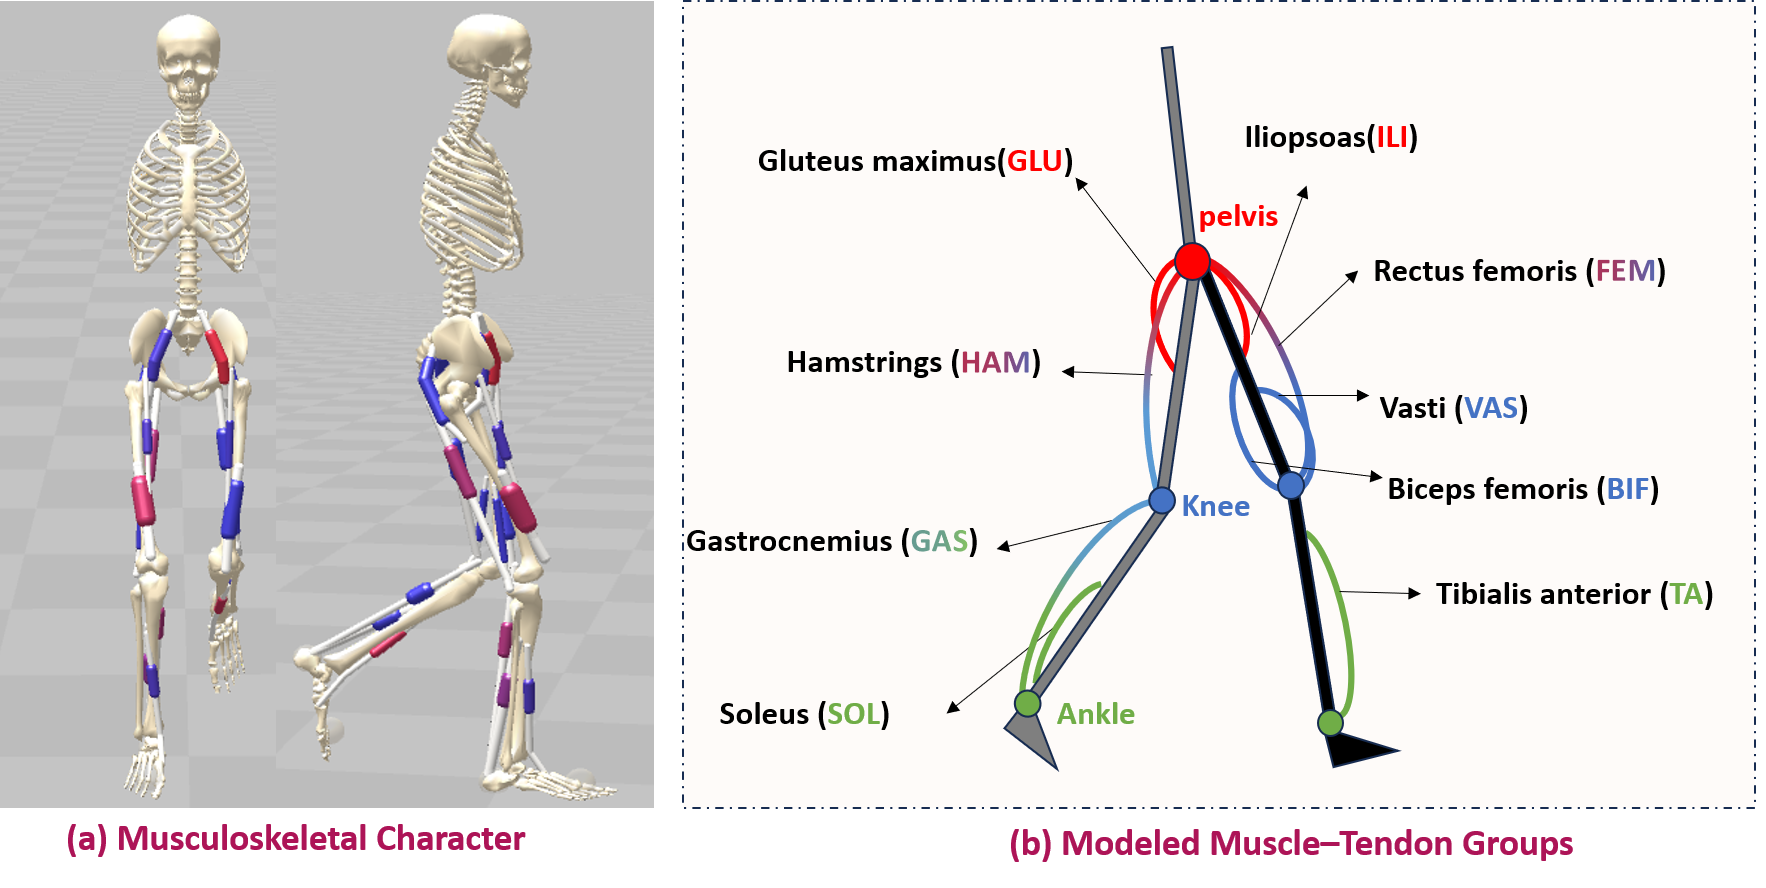
\includegraphics[width=0.76\textwidth]{musculoskeletal_character_model.png}
    \caption{Muscle-driven character model. (a) Front and sagittal views of
    the H0918v2j character used in the experiments. (b) Schematic arrangement
    and primary joint functions of the nine bilateral muscle--tendon groups.
    The complete character is actuated by 18 Hill-type muscle--tendon units,
    with one instance of each modeled group on each leg.}
    \Description{Front and side views of the musculoskeletal character beside
    a schematic of the nine bilateral muscle--tendon groups spanning the hip,
    knee, and ankle.}
    \label{fig:msk-character}
\end{figure*}

\subsubsection{Simulation platform and character.}
The physiological environment module (b) is implemented in the Hyfydy musculoskeletal simulation engine \cite{hyfydy} through the Python-based SCONE Gym interface \cite{geijtenbeek2019}. We use the sagittal-plane H0918v2j human model, which consists of a pelvis, a rigidly attached torso, and bilateral thigh, shank, and foot segments with nine generalized coordinates. The character is actuated by 18 Hill-type muscle–tendon units representing nine muscle groups on each leg, including tibialis anterior (TA), soleus (SOL), gastrocnemius (GAS), vasti (VAS), biceps femoris short head (BIF), rectus femoris (FEM), iliopsoas (ILI), hamstrings (HAM), and gluteus maximus (GLU). Each foot interacts with the ground through spherical heel and toe contact elements, and the controller is updated at 0.005 s intervals. Figure~\ref{fig:msk-character}(a) illustrates the musculoskeletal character, while Fig.~\ref{fig:msk-character}(b) summarizes the arrangement of the modeled muscle–tendon units and the joints they span.

% The physiological environment in module (b) is implemented with the Hyfydy
% musculoskeletal simulation engine \cite{hyfydy} through a Python-based
% SCONE Gym interface. We use the sagittal-plane H0918v2j human model, which
% contains a pelvis, a rigidly attached torso, and bilateral thigh, shank, and
% foot segments. Its nine generalized coordinates comprise horizontal and
% vertical pelvis translation, pelvis tilt, and bilateral hip flexion, knee
% flexion, and ankle plantarflexion--dorsiflexion. The character is actuated by
% 18 Hill-type muscle--tendon units, corresponding to nine muscle groups on each
% leg: tibialis anterior (TA), soleus (SOL), gastrocnemius (GAS), vasti (VAS),
% biceps femoris short head (BIF), rectus femoris (FEM), iliopsoas (ILI),
% hamstrings (HAM), and gluteus maximus (GLU). Each foot interacts with the
% rigid ground through spherical heel and toe contact elements. The controller
% is updated at fixed 0.005s intervals. Figure~\ref{fig:msk-character}(a) shows
% the simulated character, while Fig.~\ref{fig:msk-character}(b) summarizes the
% modeled muscle--tendon paths and their principal joint actions.

\subsubsection{Muscle-driven dynamics.}
Within module (b), reflex-generated stimulation is applied to the character
through activation dynamics, muscle--tendon mechanics, and forward dynamics. For muscle $i$, neural stimulation $u_i$ is first filtered by
activation dynamics to obtain activation $\alpha_i$, after which the Hill-type muscle model computes the corresponding muscle–tendon force
\begin{equation}
\dot{\alpha}_i=\mathcal{A}_i(\alpha_i,u_i), \qquad
F_i^{\mathrm{MT}}=\mathcal{F}_i(\alpha_i,l_i,\dot l_i),
\end{equation}
where $\mathcal{A}_i$ denotes the activation dynamics and $\mathcal{F}_i$
denotes the Hill-type muscle model. Muscle forces are then transformed into generalized joint moments through configuration-dependent muscle moment arms,
\begin{equation}
\tau_{\mathrm{mus},k}=
\sum_{i\in\mathcal{M}_k}r_{i,k}(\mathbf{q})F_i^{\mathrm{MT}},
\end{equation}
where $r_{i,k}(\mathbf{q})$ is the configuration-dependent muscle moment arm of muscle i about generalized coordinate
$k$, and $\mathcal{M}_k$ denotes the set of muscles spanning that coordinate. Finally, the generalized muscle moments drive the musculoskeletal system through forward dynamics,
\begin{equation}
\mathbf{M}(\mathbf{q})\ddot{\mathbf{q}}+
\mathbf{h}(\mathbf{q},\dot{\mathbf{q}})=
\boldsymbol{\tau}_{\mathrm{mus}}+
\mathbf{J}_{c}^{\mathsf{T}}\mathbf{f}_{c},
\end{equation}
where $\mathbf{q}$, $\dot{\mathbf{q}}$, and $\ddot{\mathbf{q}}$ are the
generalized coordinates, velocities, and accelerations, respectively;
$\mathbf{M}(\mathbf{q})$ is the mass matrix; $\mathbf{h}(\mathbf{q},\dot{\mathbf{q}})$ collects gravitational, Coriolis,
and centrifugal terms; $\boldsymbol{\tau}_{\mathrm{mus}}$ denotes the generalized joint moments generated by the muscles; $\mathbf{J}_{c}$ is the contact Jacobian; and $\mathbf{f}_{c}$ denotes the foot--ground contact forces.

\subsection{Neuromuscular Control Mechanism}
\subsubsection{Physiological feedback}
The reflex controller computes muscle stimulation from delayed muscle sensory feedback and posture feedback. Muscle length and velocity approximate muscle-spindle feedback, whereas muscle force approximates Golgi tendon organ feedback \cite{grillner2020}. These sensory signals form the physiological inputs to the reflex controller. The corresponding gains, thresholds, source muscles, target muscles, and active gait phases are defined in the following sections. As illustrated in Fig.~\ref{framwork}(b2), the resulting muscle stimulation drives activation and muscle–tendon force, while the updated muscle states provide sensory feedback for the next control step.
% The low-level controller computes muscle stimulation from delayed, normalized
% muscle length, velocity, and force signals together with posture feedback.
% Length and velocity terms represent muscle-spindle feedback, and force terms
% represent Golgi-tendon-organ feedback \cite{grillner2020}. Their gains,
% thresholds, source muscles, target muscles, and active gait phases are specified
% explicitly below. As shown in Fig.~\ref{framwork}(b2), the resulting stimulation
% $u_i$ drives activation and muscle--tendon force; the updated muscle length,
% velocity, and force then provide the next feedback sample.
\subsubsection{Phase-dependent topology.}
A finite-state controller divides the gait cycle into five phases: \textbf{Early Stance}, \textbf{Late Stance}, \textbf{Liftoff}, \textbf{Swing}, and \textbf{Landing}. Reflex pathways are organized into an all-phase group, a stance group, and a swing-related group:
\begin{equation*}
\begin{aligned}
\Phi_{\mathrm{all}} &= \{\mathrm{ES,LS,LF,SW,LA}\},\\
\Phi_{\mathrm{st}}  &= \{\mathrm{ES,LS}\},\\
\Phi_{\mathrm{sw}}  &= \{\mathrm{LF,SW,LA}\}.
\end{aligned}
\end{equation*}
Parameters are shared among phases within the same group but remain independent across groups. For example, the BIF force-feedback gain used during Early Stance and Late Stance differs from that used during Liftoff, Swing, and Landing, allowing the same sensory feedback to support different functions, including stance support, push-off, and swing control, without requiring a separate parameter for every gait phase. Fig.~\ref{framwork}(b1) summarizes the resulting topology across the nine modeled muscle groups. Monoarticular pathways involve TA and SOL at the ankle, VAS and BIF at the knee, and ILI and GLU at the hip. The biarticular muscles GAS, FEM, and HAM span two adjacent joints and therefore contribute to the control of both.


The active parameter-sharing groups are determined by the current gait phase. During Early Stance and Late Stance, the controller activates the all-phase and stance-specific pathways, whereas during Liftoff, Swing, and Landing, it activates the all-phase and swing-related pathways. For convenience, let $\phi(t)$ denote the current gait phase and $\Gamma(\phi)$ the corresponding set of active parameter-sharing groups, such that $\Gamma(\phi)=\{\mathrm{all},\mathrm{st}\}$ during Early Stance and $\Gamma(\phi)=\{\mathrm{all},\mathrm{sw}\}$ during Liftoff, Swing, and Landing.

Each active parameter-sharing group $g\in\Gamma(\phi)$ defines a sparse directed feedback graph $\mathcal{G}_{g}$. A connection $i\leftarrow j$ uses sensory feedback measured from source muscle $j$ to modulate the stimulation of target muscle $i$. Connections with $i=j$ implement self-feedback, whereas connections with $i\neq j$  encode inter-muscle coordination. Reflex gains and thresholds are indexed by the active parameter-sharing group, while inactive pathways have zero gain during the corresponding gait phases. The sign and magnitude of each gain determine how strongly the corresponding sensory feedback facilitates or suppresses the target muscle stimulation.


\subsubsection{Reflex control laws.}
For an active group $g\in\Gamma(\phi(t))$, muscle stimulation is computed from muscle length, velocity, and force feedback.
\begin{align}
u_{L,i\leftarrow j}^{(g)}(t) &= K_{L,i\leftarrow j}^{(g)}
\max(0,\tilde{l}_j(t-t_D)-\tilde{l}_{0,i\leftarrow j}^{(g)}),\\
u_{V,i\leftarrow j}^{(g)}(t) &= K_{V,i\leftarrow j}^{(g)}
\max(0,\tilde{v}_j(t-t_D)-\tilde{v}_{0,i\leftarrow j}^{(g)}),\\
u_{F,i\leftarrow j}^{(g)}(t) &= K_{F,i\leftarrow j}^{(g)}
(\tilde{f}_j(t-t_D)-\tilde{f}_{0,i\leftarrow j}^{(g)}),
\end{align}
where $\tilde{l}_j$, $\tilde{v}_j$, and $\tilde{f}_j$ denote delayed normalized muscle length, velocity, and force measured from source muscle $j$, respectively. The corresponding gains $K_{L}$, $K_{V}$, and $K_{F}$ and thresholds $\tilde{l}_{0}$, $\tilde{v}_{0}$, and $\tilde{f}_{0}$ are indexed by the active parameter-sharing group $g$, and $t_D$ is the sensorimotor delay.

A reflex-like postural feedback term is also used to couple trunk pitch
errors to selected lower-limb muscles.
\begin{equation}
u_{\text{PD},i}^{(g)}(t)=
K_{P,i}^{(g)}(\theta(t-t_D)-\theta_{0,i}^{(g)})+
K_{D,i}^{(g)}\dot{\theta}(t-t_D).
\end{equation}
where $\theta$ and $\dot{\theta}$ are the delayed trunk pitch angle and angular
velocity, $\theta_{0,i}^{(g)}$ is the target pitch offset for muscle $i$, and
$K_{P,i}^{(g)}$ and $K_{D,i}^{(g)}$ are the proportional and derivative
postural-feedback gains for the active group.

The total muscle stimulation of muscle $i$ is obtained by summing the constant background stimulation, muscle sensory feedback and postural feedback contributions from all active parameter-sharing groups.
\begin{equation}
\begin{aligned}
u_i(t) = \sum_{g\in\Gamma(\phi(t))}\Bigg[
&u_{C,i}^{(g)}+u_{\text{PD},i}^{(g)}(t)\\
&+\sum_{j\in\mathcal{M}_{g}}\left(u_{L,i\leftarrow j}^{(g)}(t)
+u_{V,i\leftarrow j}^{(g)}(t)+u_{F,i\leftarrow j}^{(g)}(t)\right)\Bigg].
\end{aligned}
\end{equation}
where $u_{C,i}^{(g)}$ is the group-dependent constant background stimulation and
$\mathcal{M}_{g}$ is the set of source muscles connected to target $i$ in the
corresponding active group. The resulting muscle stimulation drives the activation dynamics and musculoskeletal model described in Sec.~\ref{sec:musculoskeletal-model}.

\subsection{Residual Neuromuscular Regulation}

\subsubsection{Residual formulation}
Rather than directly generating muscle stimulation, the reinforcement learning policy regulates the underlying neuromuscular controller through a four-dimensional residual action $\mathbf{a}_t\in\mathbb{R}^{4}$. Each action component modulates one selected reflex parameter around its nominal value,
\begin{equation}
p_i(t)=p_{i,0}(1+\lambda a_i(t)),
\label{eq:residual_scaling}
\end{equation}
where $p_{i,0}$ is the nominal reflex parameter and $\lambda$  is the action scale. In the present implementation, $\lambda=0.5$. When $a_i(t)=0$, the nominal reflex controller is recovered exactly, whereas nonzero actions produce state-dependent modulation of the selected reflex parameters. The resulting muscle stimulation is then computed by the underlying neuromuscular controller using the current muscle sensory feedback, gait phase, and the regulated reflex parameters.

\begin{table}[!t]
\caption{Selected Residual-Reflex Actions}
\label{tab:residual_actions}
\centering
\small
\setlength{\tabcolsep}{3pt}
\renewcommand{\arraystretch}{1.12}
\begin{tabularx}{\columnwidth}{c c c X}
\toprule
\textbf{Action} & \textbf{Parameter} & \textbf{Pathway} & \textbf{Functional role} \\
\midrule
$a_1$ & $K_{L,\mathrm{HAM}}^{(\mathrm{sw})}$ & S11100.hamstrings.KL & Hip extension / knee flexion \\
$a_2$ & $\tilde{l}_{0,\mathrm{ILI}}^{(\mathrm{st})}$ & S00011.iliopsoas.L0 & Hip flexion / leg advancement \\
\textbf{$a_3$} & \textbf{$K_{F,\mathrm{SOL}}^{(\mathrm{all})}$} & \textbf{S11111.soleus.KF} & \textbf{Ankle support / propulsion} \\
$a_4$ & $K_{F,\mathrm{VAS}}^{(\mathrm{st})}$ & S00011.vasti.KF & Knee extension / stance support \\
\bottomrule
\end{tabularx}
\end{table}

\subsubsection{Regulated reflex parameters}

The four regulated parameters are highlighted in bright magenta in Fig.~\ref{framwork}(b1), and their corresponding pathways are summarized in Table~\ref{tab:residual_actions}. In Table~\ref{tab:residual_actions}, pathway labels follow the naming convention of the controller implementation, while the superscripts (all), (st), and (sw) explicitly indicate the corresponding phase groups used in this paper. Specifically, $a_1$ modulates the swing-related hamstrings length gain to regulate hip extension and knee flexion during leg swing, $a_2$ adjusts the stance-phase iliopsoas length threshold for hip flexion and leg advancement, $a_3$ modulates the all-phase soleus force-feedback gain for ankle support and propulsion, and $a_4$ regulates the stance-phase vasti force-feedback gain for knee extension and stance support.

These four parameters were selected because they regulate gait-critical functions across the major lower-limb joints while directly influencing the key biomechanical roles required for locomotion, including leg swing, stance support, and propulsion. By restricting policy outputs to these biomechanically meaningful reflex parameters, the proposed formulation concentrates policy exploration on neuromuscular mechanisms that are directly related to locomotor function while maintaining a compact and interpretable action space.


\subsection{Policy Learning with MPO}

Policy learning follows an off-policy actor–critic framework optimized with Maximum a Posteriori Policy Optimization (MPO) \cite{mpo2018}. As illustrated in Fig.~\ref{framwork}(c), the actor receives the current musculoskeletal observation and outputs a four-dimensional residual action, while the critic evaluates the corresponding state–action pair. Let $\mathbf{s}_t\in\mathbb{R}^{121}$  denote the observation at time $t$,
\begin{equation}
\begin{aligned}
\mathbf{s}_t = [
&\mathbf{l}_t,\dot{\mathbf{l}}_t,\mathbf{f}_t,\mathbf{e}_t,\boldsymbol{\alpha}_t,\mathbf{p}_{feet,t},\mathbf{q}_t,\dot{\mathbf{q}}_t].
\end{aligned}
\end{equation}
Here $\mathbf{l}$, $\dot{\mathbf{l}}$, and $\mathbf{f}$ are muscle-fiber
lengths, velocities, and forces; $\mathbf{e}$ and $\boldsymbol{\alpha}$ are
muscle excitations and activations; $\mathbf{p}_{feet}$ represents foot
positions relative to the pelvis; $\mathbf{q}$ and
$\dot{\mathbf{q}}$ denote the pelvis and joint degrees of freedom and their corresponding velocities, respectively.


The actor and critic are implemented as multilayer perceptrons with two hidden layers of 256 ReLU units. The actor $\pi(\mathbf{s};\boldsymbol{\theta}_{\mathrm{now}})$ predicts the mean and standard deviation of a Gaussian policy, from which a four-dimensional residual action is sampled during training. During evaluation, the deterministic policy uses the action mean. The critic $q(\mathbf{s},\mathbf{a};\boldsymbol{\omega})$ estimates the corresponding action-value function $Q(\mathbf{s},\mathbf{a})$.

Transitions $(\mathbf{s}_t,\mathbf{a}_t,r_t,\mathbf{s}_{t+1})$ are stored in a replay buffer $\mathcal{D}$. MPO updates the critic from replayed transitions and optimizes the actor under a KL-divergence constraint, enabling stable off-policy learning while reusing collected experience. We follow the standard MPO update procedure and therefore omit the derivation here.

Policy optimization is driven by the following reward function, which consists of a target-speed reward $r_v$ together with penalty terms for excessive contact loading ($c_{grf}$), temporal excitation variation ($c_e$), unnecessary muscle recruitment ($c_m$), joint-limit loading ($c_q$), pelvis instability ($c_{\theta},c_{\dot\theta},c_{com}$), and rapid changes in the residual parameter increments ($c_{\Delta p}$)


\begin{equation}
\begin{aligned}
r_t={}&w_v r_v
-\lambda_{grf}c_{grf}-\lambda_e c_e-\lambda_m c_m
-\lambda_q c_q\\
&-\lambda_{\theta}c_{\theta}
-\lambda_{\dot\theta}c_{\dot\theta}
-\lambda_{com}c_{com}-\lambda_{\Delta p}c_{\Delta p},
\end{aligned}
\end{equation}
The target-speed reward is defined as
\begin{equation}
r_v=\begin{cases}
\exp[-(v_x-v^*)^2], & v_x<v^*,\\
1, & v_x\ge v^*.
\end{cases}
\end{equation}
where $v_x$ and $v^*$ denote the forward center-of-mass speed and the commanded speed, respectively. The individual penalty terms are defined as
\begin{equation}
\begin{aligned}
c_{grf}&=[L_c-1.2]_+,\\
c_e&=\frac{1}{N}\|\mathbf e_t-\mathbf e_{t-1}\|_2^2,\\
c_m&=\frac{1}{d_a}\sum_{i=1}^{N}
\mathbb{I}\!\left[\alpha_i>0.15\right],\\
c_q&=\frac{1}{J}\sum_{j=1}^{J}
\operatorname{mean}\!\left(\left|\boldsymbol{\tau}^{\mathrm{lim}}_j\right|\right).
\end{aligned}
\label{eq:reward_cost1}
\end{equation}
where $L_c$ is the total contact load normalized by body weight; $N$ is the
number of muscles; $d_a$ is the action-space dimension; $J$ is the number of
joints; $\boldsymbol{\tau}^{\mathrm{lim}}_j$ is the joint-limit torque of joint
$j$; $\mathbb{I}[\cdot]$ is the indicator function; and
$[x]_+=\max(0,x)$.
\begin{equation}
\begin{aligned}
c_\theta &= (\theta_t-\theta^*)^2,\\
c_{\dot\theta} &= \dot{\theta}_t^{\,2},\\
c_{com} &= (v_{com,y})^2,\\
\boldsymbol{\delta p}_t &= \lambda\mathbf{p}_0\odot\mathbf{a}_t,\\
c_{\Delta p} &= \frac14\|\boldsymbol{\delta p}_t-\boldsymbol{\delta p}_{t-1}\|_2^2.
\end{aligned}
\label{eq:reward_cost3}
\end{equation}
where $\theta^*$ is the target pelvis pitch; $v_{com,y}$ is the vertical center-of-mass velocity; $\mathbf a_t$ denotes the four-dimensional residual action produced by the policy; $\mathbf p_0$ collects the corresponding nominal reflex parameters; $\odot$ denotes element-wise multiplication; and $\boldsymbol{\delta p}_t$ is the vector of residual parameter increments applied at time $t$.


\section{Evaluation}
\label{sec:evaluation-protocol}

\subsection{Evaluation Protocol}
\subsubsection{Experimental Setup}
The simulator, musculoskeletal character, muscle-driven dynamics, and
foot--ground contact model are described in Sec.~\ref{sec:musculoskeletal-model}. The same character and
simulation settings were used for all controllers unless a plantarflexor
weakness condition was explicitly introduced.

The evaluation includes four control approaches: two direct muscle-control
reinforcement learning methods, E2E-RL \cite{weng2021,devree2021,ogum2024}
and DEP-RL \cite{deprl2023}; the proposed Residual-Reflex RL method; and a
reflex controller whose parameters were optimized offline using CMA-ES.
Table~\ref{tab:policy_interface} summarizes the policy interfaces of the
three reinforcement learning methods. The CMA-ES baseline has no learned
policy output and keeps its optimized reflex parameters fixed during
evaluation. All reinforcement learning policies were trained using the same MPO framework and musculoskeletal model. Training was performed on a workstation equipped with an AMD Ryzen Threadripper PRO 9965WX CPU and 256 GB RAM.

\begin{table}[!t]
\centering
\caption{Policy interfaces of the reinforcement learning methods.}
\label{tab:policy_interface}
\small
\setlength{\tabcolsep}{4pt}
\renewcommand{\arraystretch}{1.15}
\begin{tabularx}{\linewidth}{l c X}
\toprule
\textbf{Method} & \textbf{Action dim.} & \textbf{Policy output} \\
\midrule
E2E-RL & 18 & Direct muscle-level control actions. \\
DEP-RL & 18 & Direct muscle-level control with DEP-style embodied exploration. \\
\textbf{Residual-Reflex RL} & \textbf{4} & \textbf{Residual modulation of selected reflex parameters.} \\
\bottomrule
\end{tabularx}
\end{table}

\subsubsection{Tasks and Evaluation Metrics}
The evaluation consists of three complementary experiments designed to assess both physiological plausibility and adaptability. Nominal walking evaluates gait quality under controlled target-speed tasks, plantarflexor weakness evaluates adaptation to changes in musculoskeletal capacity, and external push perturbation evaluates recovery from environmental disturbances.

For nominal walking, policies were evaluated at target walking speeds of 0.8, 1.0, and 1.2 m/s. Each policy was simulated for 25 s, and the resulting trajectories were exported as STO files for post-hoc gait analysis. All detected gait cycles were normalized to 0–100\% of the gait cycle. The comparison includes E2E-RL, DEP-RL, and Residual-Reflex RL. Four groups of metrics are used to evaluate task performance, physiological plausibility, and gait consistency.

\paragraph{Speed tracking and stride measures}
To evaluate task performance, we report
realized walking speed, absolute speed error
$|\hat{v}-v_{\mathrm{target}}|$, stride length, stride time, and the number of analyzed cycles. The realized walking speed and speed error quantify how accurately the controller follows the commanded locomotion task, whereas stride length and stride time characterize the gait strategy adopted to achieve the target speed.

\paragraph{Human-reference kinematic gait score}
To evaluate kinematic plausibility, we compare the generated gait-cycle profiles with human-reference kinematic data for the hip, knee, and ankle joints. These reference profiles are used only for offline evaluation and are not included in the reinforcement learning reward. For each joint, left and right gait cycles were time-normalized and averaged to obtain a mean simulated profile $\bar{y}(x)$, where $x$ denotes the normalized gait-cycle percentage. Let $y_{\min}(x_k)$ and $y_{\max}(x_k)$ denote the lower and upper human-reference bounds at sample point $x_k$. The normalized reference-range violation is
\begin{equation}
e = \frac{1}{N}\sum_{k=1}^{N}
\frac{
\left[y_{\min}(x_k)-\bar{y}(x_k)\right]_+
+ \left[\bar{y}(x_k)-y_{\max}(x_k)\right]_+
}{
\max\left(0.01, y_{\max}(x_k)-y_{\min}(x_k)\right)
},
\label{eq:reference_range_violation}
\end{equation}
where $[z]_+=\max(z,0)$.
The corresponding score is
\begin{equation}
S = 100 \cdot \mathrm{clip}(1-e,0,1).
\end{equation}
Higher scores indicate closer agreement with the human-reference gait profiles. A score of 100 indicates that the averaged trajectory remains entirely within the reference range. The overall kinematic score is computed as the average of the hip, knee, and ankle scores.

\paragraph{Vertical GRF human-reference score}
To evaluate dynamic plausibility, we analyze the vertical ground reaction force (GRF), which directly reflects body loading and push-off behavior. Individual left and right GRF gait cycles are visualized to assess stance-phase loading patterns, double-support and propulsion behavior, and stride-to-stride consistency. The numerical GRF score is computed using the human-reference range metric in Eq.~\ref{eq:reference_range_violation}, applied to the vertical GRF profile, whereas the waveform plots provide a qualitative comparison of left–right symmetry and stride-to-stride repeatability.

\paragraph{Symmetry and repeatability score}
To evaluate gait consistency and repeatability, we quantify bilateral symmetry and stride-to-stride repeatability. Bilateral symmetry is measured as the root-mean-square (RMS) difference between the average left and right normalized gait-cycle waveforms. For a gait-cycle quantity $y$, this waveform difference is
\begin{equation}
D_y =
\sqrt{\frac{1}{N}\sum_{k=1}^{N}
\left(\bar{y}_{L}(x_k)-\bar{y}_{R}(x_k)\right)^2},
\end{equation}
where $y$ denotes a normalized gait-cycle waveform, $x_k$ is the $k$th
gait-cycle sample, $N$ is the number of samples in the normalized gait cycle,
and $\bar{y}_{L}$ and $\bar{y}_{R}$ are the average left- and right-side
profiles computed over the analyzed cycles. In the results, lower $D_y$
indicates more symmetric left--right motion.
Stride-to-stride repeatability is quantified using the coefficient of variation (CV) of stride time and stride length,
\begin{equation}
\mathrm{CV}_{z}=100\frac{\sigma_z}{\mu_z},
\end{equation}
where $z$ denotes either stride time or stride length, $\mu_z$ is the mean
value of $z$, and $\sigma_z$ is its standard deviation over the analyzed gait
cycles. The factor 100 expresses the coefficient of variation as a percentage. Lower $\mathrm{CV}_z$ indicates more repeatable gait cycles.
In the reported results, the Hip, Knee, Ankle, and GRF columns correspond to $D_y$ for the respective left–right waveform pairs, whereas the Time CV and Length CV columns report $\mathrm{CV}_z$ for stride time and stride length, respectively.

\subsection{Nominal Gait Generation}
This experiment evaluates whether the proposed controller generates physiologically plausible locomotion under nominal walking conditions. Three controllers (E2E-RL, DEP-RL, and Residual-Reflex RL) are compared at target walking speeds of 0.8, 1.0, and 1.2 m/s. The evaluation proceeds from task performance to kinematic plausibility, dynamic plausibility, gait consistency, and qualitative motion analysis.

\label{sec:nominal-gait}
\subsubsection{Task Performance}
The speed tracking and stride measures show that all three controllers successfully generated sustained forward walking under the commanded speed tasks. As summarized in Table~\ref{tab:spatiotemporal_metrics}, Residual-Reflex RL achieved the most accurate speed tracking at all target speeds, with absolute speed errors of 0.01, 0.05, and 0.01 m/s at 0.8, 1.0, and 1.2 m/s, respectively. E2E-RL and DEP-RL also completed all walking tasks, but exhibited larger speed errors, particularly at higher target speeds where both methods tended to overshoot the commanded velocity.

These results establish that the subsequent comparisons are performed among controllers that all accomplish the locomotion task, rather than between successful and failed walking trials. The stride measures further reveal different gait strategies. E2E-RL tends to use shorter and faster steps at lower walking speeds, whereas DEP-RL and Residual-Reflex RL adopt longer strides. The following analyses therefore investigate whether successful task execution is also accompanied by human-like kinematics, dynamic consistency, and gait consistency.

\begin{table}[!t]
\centering
\caption{Speed tracking and stride measures from the analyzed walking
trajectories. Speed error is the absolute difference between realized and target
speed.}
\label{tab:spatiotemporal_metrics}
\small
\setlength{\tabcolsep}{3.5pt}
\renewcommand{\arraystretch}{1.12}
\resizebox{\columnwidth}{!}{%
\begin{tabular}{c l r r r r r}
\toprule
\makecell{\textbf{Target}\\\textbf{speed}} & \textbf{Method} & \makecell{\textbf{Realized}\\\textbf{speed}} & \textbf{Error} & \textbf{Stride len.} & \textbf{Stride time} & \textbf{Cycles} \\
\midrule
\multirow[c]{3}{*}{0.8} & E2E-RL & 0.87 & 0.07 & 0.78 & 0.89 & 50 \\
 & DEP-RL & 0.83 & 0.03 & 1.09 & 1.31 & 33 \\
 & \textbf{Residual-Reflex RL} & 0.79 & \textbf{0.01} & 0.99 & 1.26 & 35 \\
\midrule
\multirow[c]{3}{*}{1.0} & E2E-RL & 1.18 & 0.18 & 1.39 & 1.18 & 37 \\
 & DEP-RL & 1.14 & 0.14 & 1.29 & 1.13 & 39 \\
 & \textbf{Residual-Reflex RL} & 1.05 & \textbf{0.05} & 1.23 & 1.17 & 37 \\
\midrule
\multirow[c]{3}{*}{1.2} & E2E-RL & 1.26 & 0.06 & 1.23 & 0.97 & 46 \\
 & DEP-RL & 1.30 & 0.10 & 1.37 & 1.06 & 42 \\
 & \textbf{Residual-Reflex RL} & 1.21 & \textbf{0.01} & 1.34 & 1.11 & 40 \\
\bottomrule
\end{tabular}%
}
\end{table}

\subsubsection{Joint Kinematic Plausibility}
The human-reference kinematic scores reveal a clear separation between the three controllers. As summarized in Table~\ref{tab:gait_similarity}, Residual-Reflex RL achieved the highest joint-kinematic score at all target walking speeds, with an average score of 88.0\% across the 0.8, 1.0, and 1.2 m/s evaluations. The improvement is most pronounced in the knee and ankle joints, where the proposed controller consistently preserves human-reference joint coordination. In contrast, E2E-RL maintains relatively high hip scores but exhibits less consistent knee and ankle motion, whereas DEP-RL performs consistently worse, particularly at 1.2 m/s. Fig.~\ref{fig:gait_score_bars} summarizes these quantitative comparisons across all target speeds.

Scores close to zero indicate that the averaged joint trajectory remains outside the human-reference range over most of the gait cycle, rather than exhibiting only localized deviations. This distinction is important because controllers can successfully complete the walking task while still producing joint motions that differ substantially from human gait.


\begin{table}[!t]
\centering
\caption{Human-reference kinematic scores in controlled walking validation.
Scores are computed from normalized hip, knee, and ankle gait-cycle profiles.
The kinematic average is the mean of the hip, knee, and ankle scores.}
\label{tab:gait_similarity}
\small
\setlength{\tabcolsep}{3.5pt}
\renewcommand{\arraystretch}{1.12}
\resizebox{\columnwidth}{!}{%
\begin{tabular}{c l r r r r r}
\toprule
\makecell{\textbf{Target}\\\textbf{speed}} & \textbf{Method} & \makecell{\textbf{Realized}\\\textbf{speed}} & \makecell{\textbf{Kinematic}\\\textbf{average}} & \textbf{Hip} & \textbf{Knee} & \textbf{Ankle} \\
\midrule
\multirow[c]{3}{*}{0.8} & E2E-RL & 0.87 & 39.0 & \textbf{98.3} & 18.6 & 0.0 \\
 & DEP-RL & 0.83 & 44.1 & 72.7 & 50.8 & 8.7 \\
 & \textbf{Residual-Reflex RL} & 0.79 & \textbf{81.3} & 96.6 & \textbf{68.9} & \textbf{78.5} \\
\midrule
\multirow[c]{3}{*}{1.0} & E2E-RL & 1.18 & 81.9 & 81.2 & 72.7 & \textbf{91.8} \\
 & DEP-RL & 1.14 & 58.5 & 62.5 & 64.2 & 48.7 \\
 & \textbf{Residual-Reflex RL} & 1.05 & \textbf{90.5} & \textbf{100.0} & \textbf{82.6} & 88.9 \\
\midrule
\multirow[c]{3}{*}{1.2} & E2E-RL & 1.26 & 75.6 & 88.4 & 52.4 & 85.9 \\
 & DEP-RL & 1.30 & 40.8 & 44.5 & 33.4 & 44.5 \\
 & \textbf{Residual-Reflex RL} & 1.21 & \textbf{92.3} & \textbf{99.6} & \textbf{88.7} & \textbf{88.6} \\
\bottomrule
\end{tabular}%
}
\end{table}

\begin{figure}[!t]
\centerline{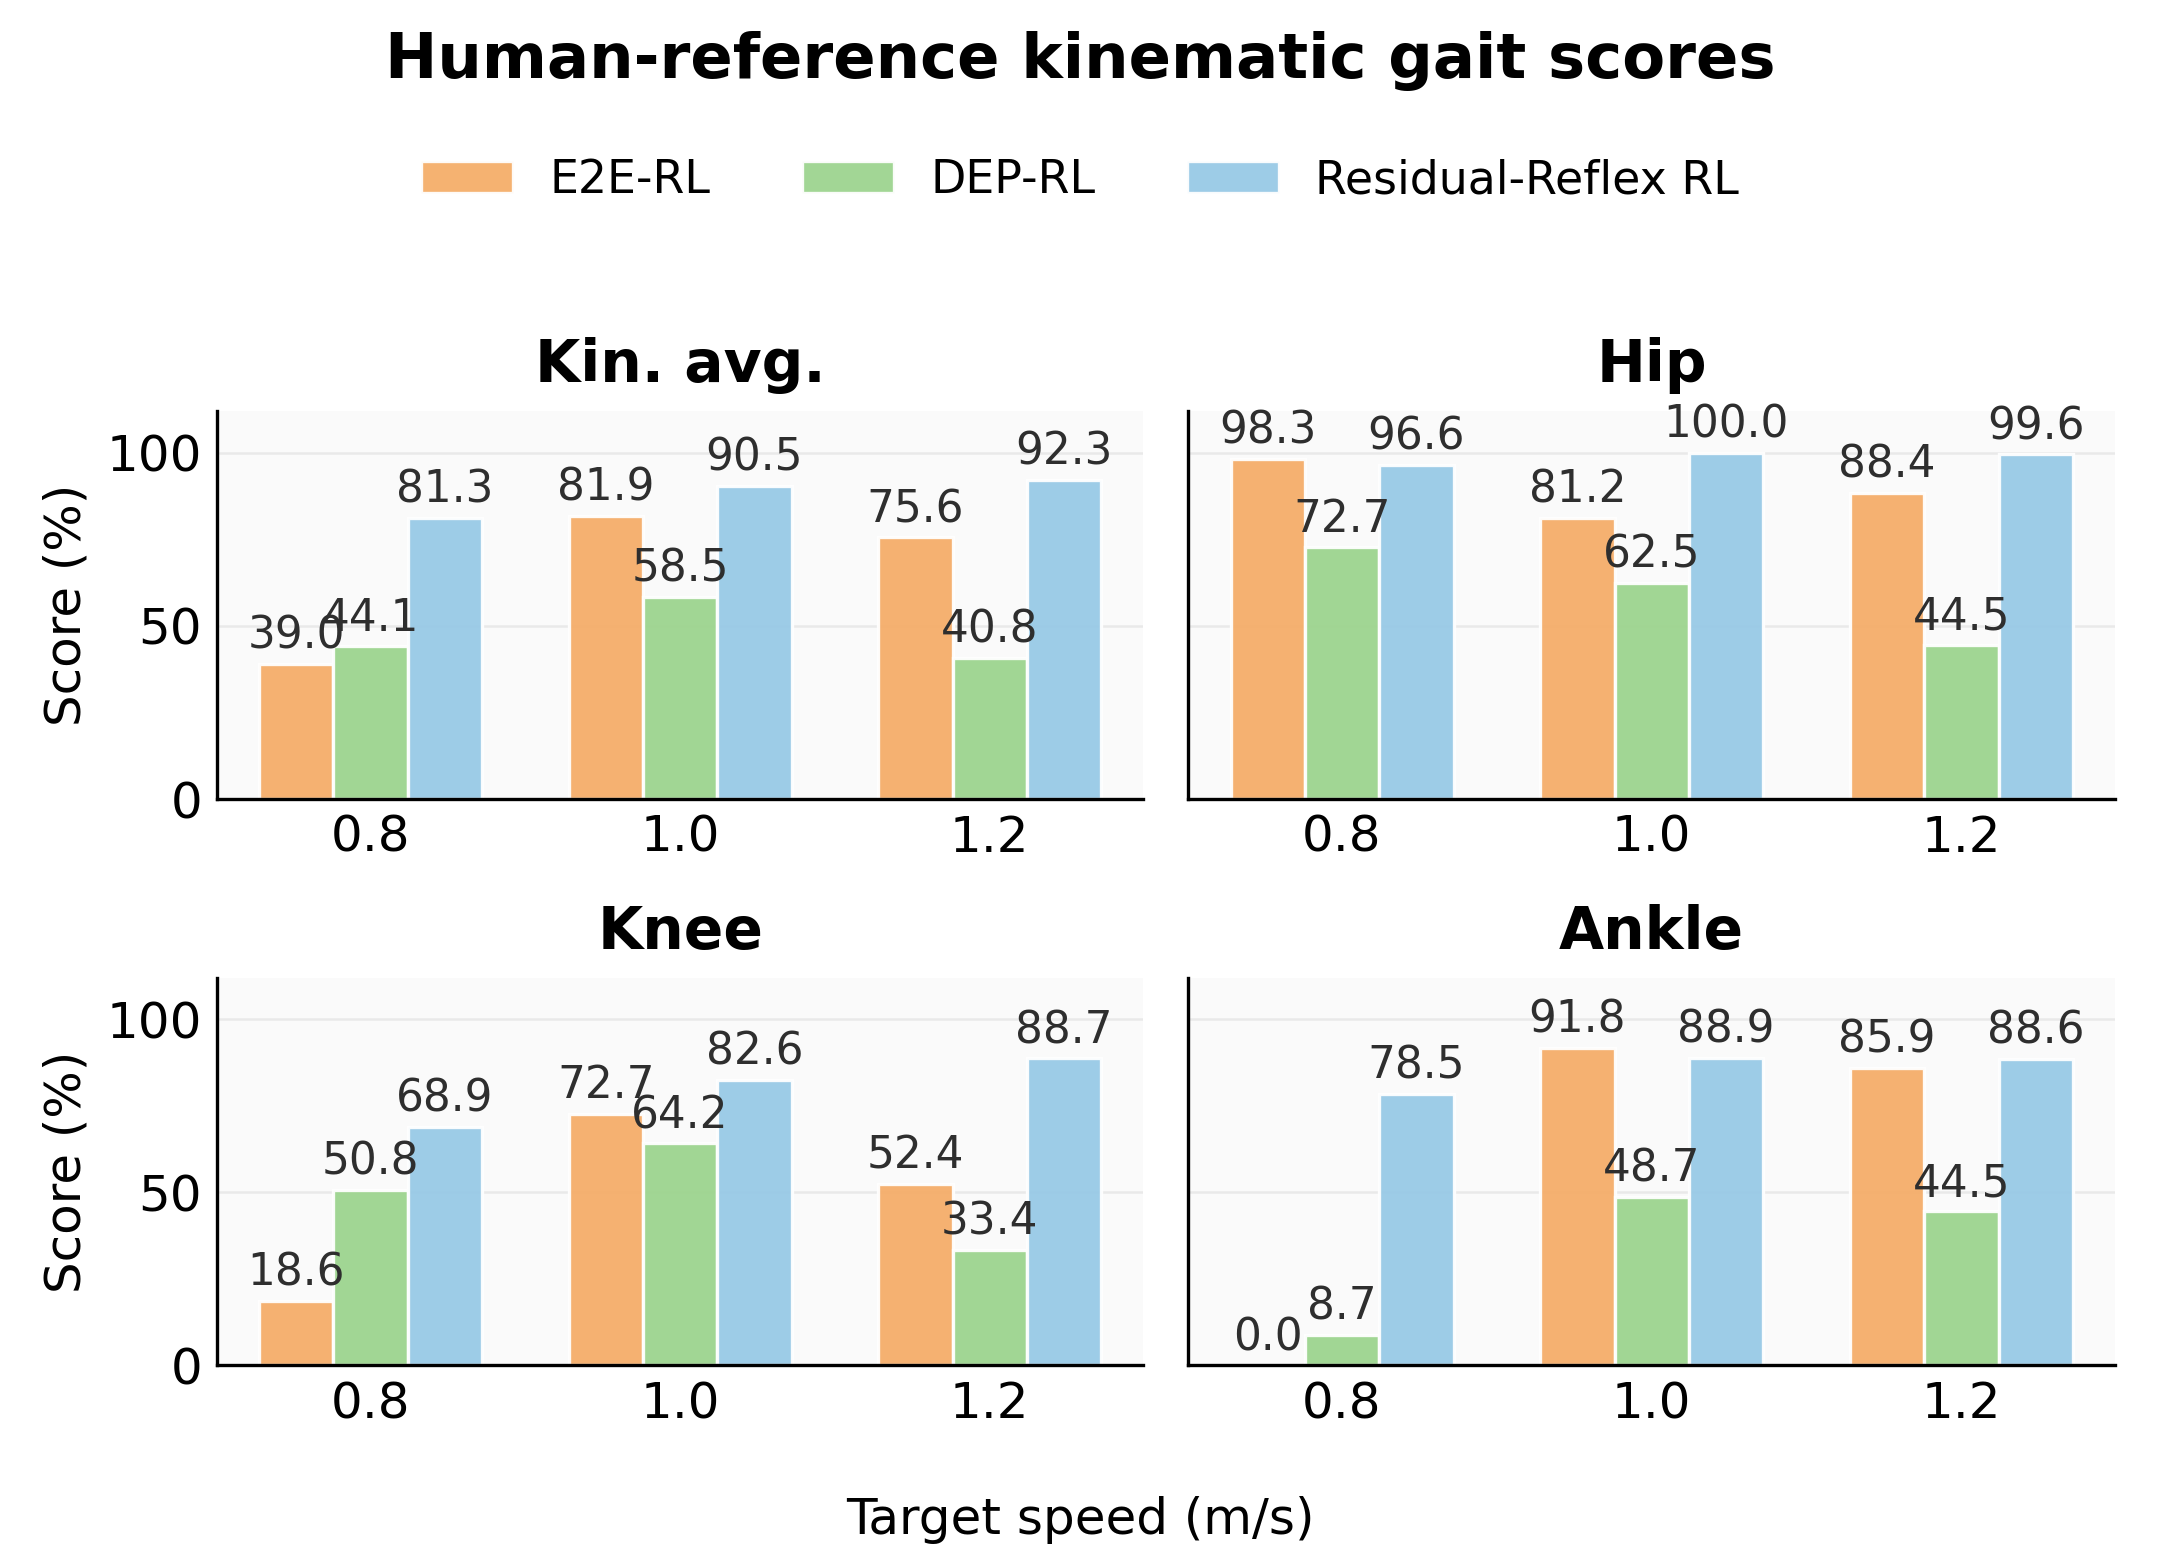
\includegraphics[width=\columnwidth]{gait_score_comparison_bars.png}}
\caption{Human-reference kinematic gait scores across target speeds. Numeric
labels indicate the score of each bar. The Residual-Reflex RL controller achieves
the highest kinematic-average score and especially improves knee and ankle
components.}
\Description{Grouped bars compare average hip, knee, and ankle kinematic scores
for three controllers at three walking speeds. Residual-Reflex RL has the
highest kinematic-average score at every speed.}
\label{fig:gait_score_bars}
\end{figure}

The waveform comparisons in Figs.~\ref{fig:gait_profiles_08}--\ref{fig:gait_profiles_12} further explain these quantitative results and illustrate how the controllers behave across different target speeds. At 0.8 m/s, E2E-RL produced a reasonable hip trajectory but failed to maintain human-reference knee and ankle profiles, whereas DEP-RL exhibited larger left–right differences and stride-to-stride variability. At 1.0 m/s, all controllers produced gait patterns closer to the reference trajectories, but Residual-Reflex RL still generated the most compact waveform distribution and the highest overall score. At 1.2 m/s, where faster stance-to-swing transitions are required, the difference became more pronounced. Residual-Reflex RL maintained knee and ankle trajectories clustered around the human-reference ranges, whereas E2E-RL and DEP-RL showed larger deviations and more scattered gait cycles.

These observations are consistent with the quantitative scores reported in Table~\ref{tab:gait_similarity} and further explain why Residual-Reflex RL produces more repeatable locomotion. The narrower distributions of the left and right gait cycles indicate more consistent joint coordination across both successive gait cycles and bilateral limbs.

\begin{figure}[!t]
\centerline{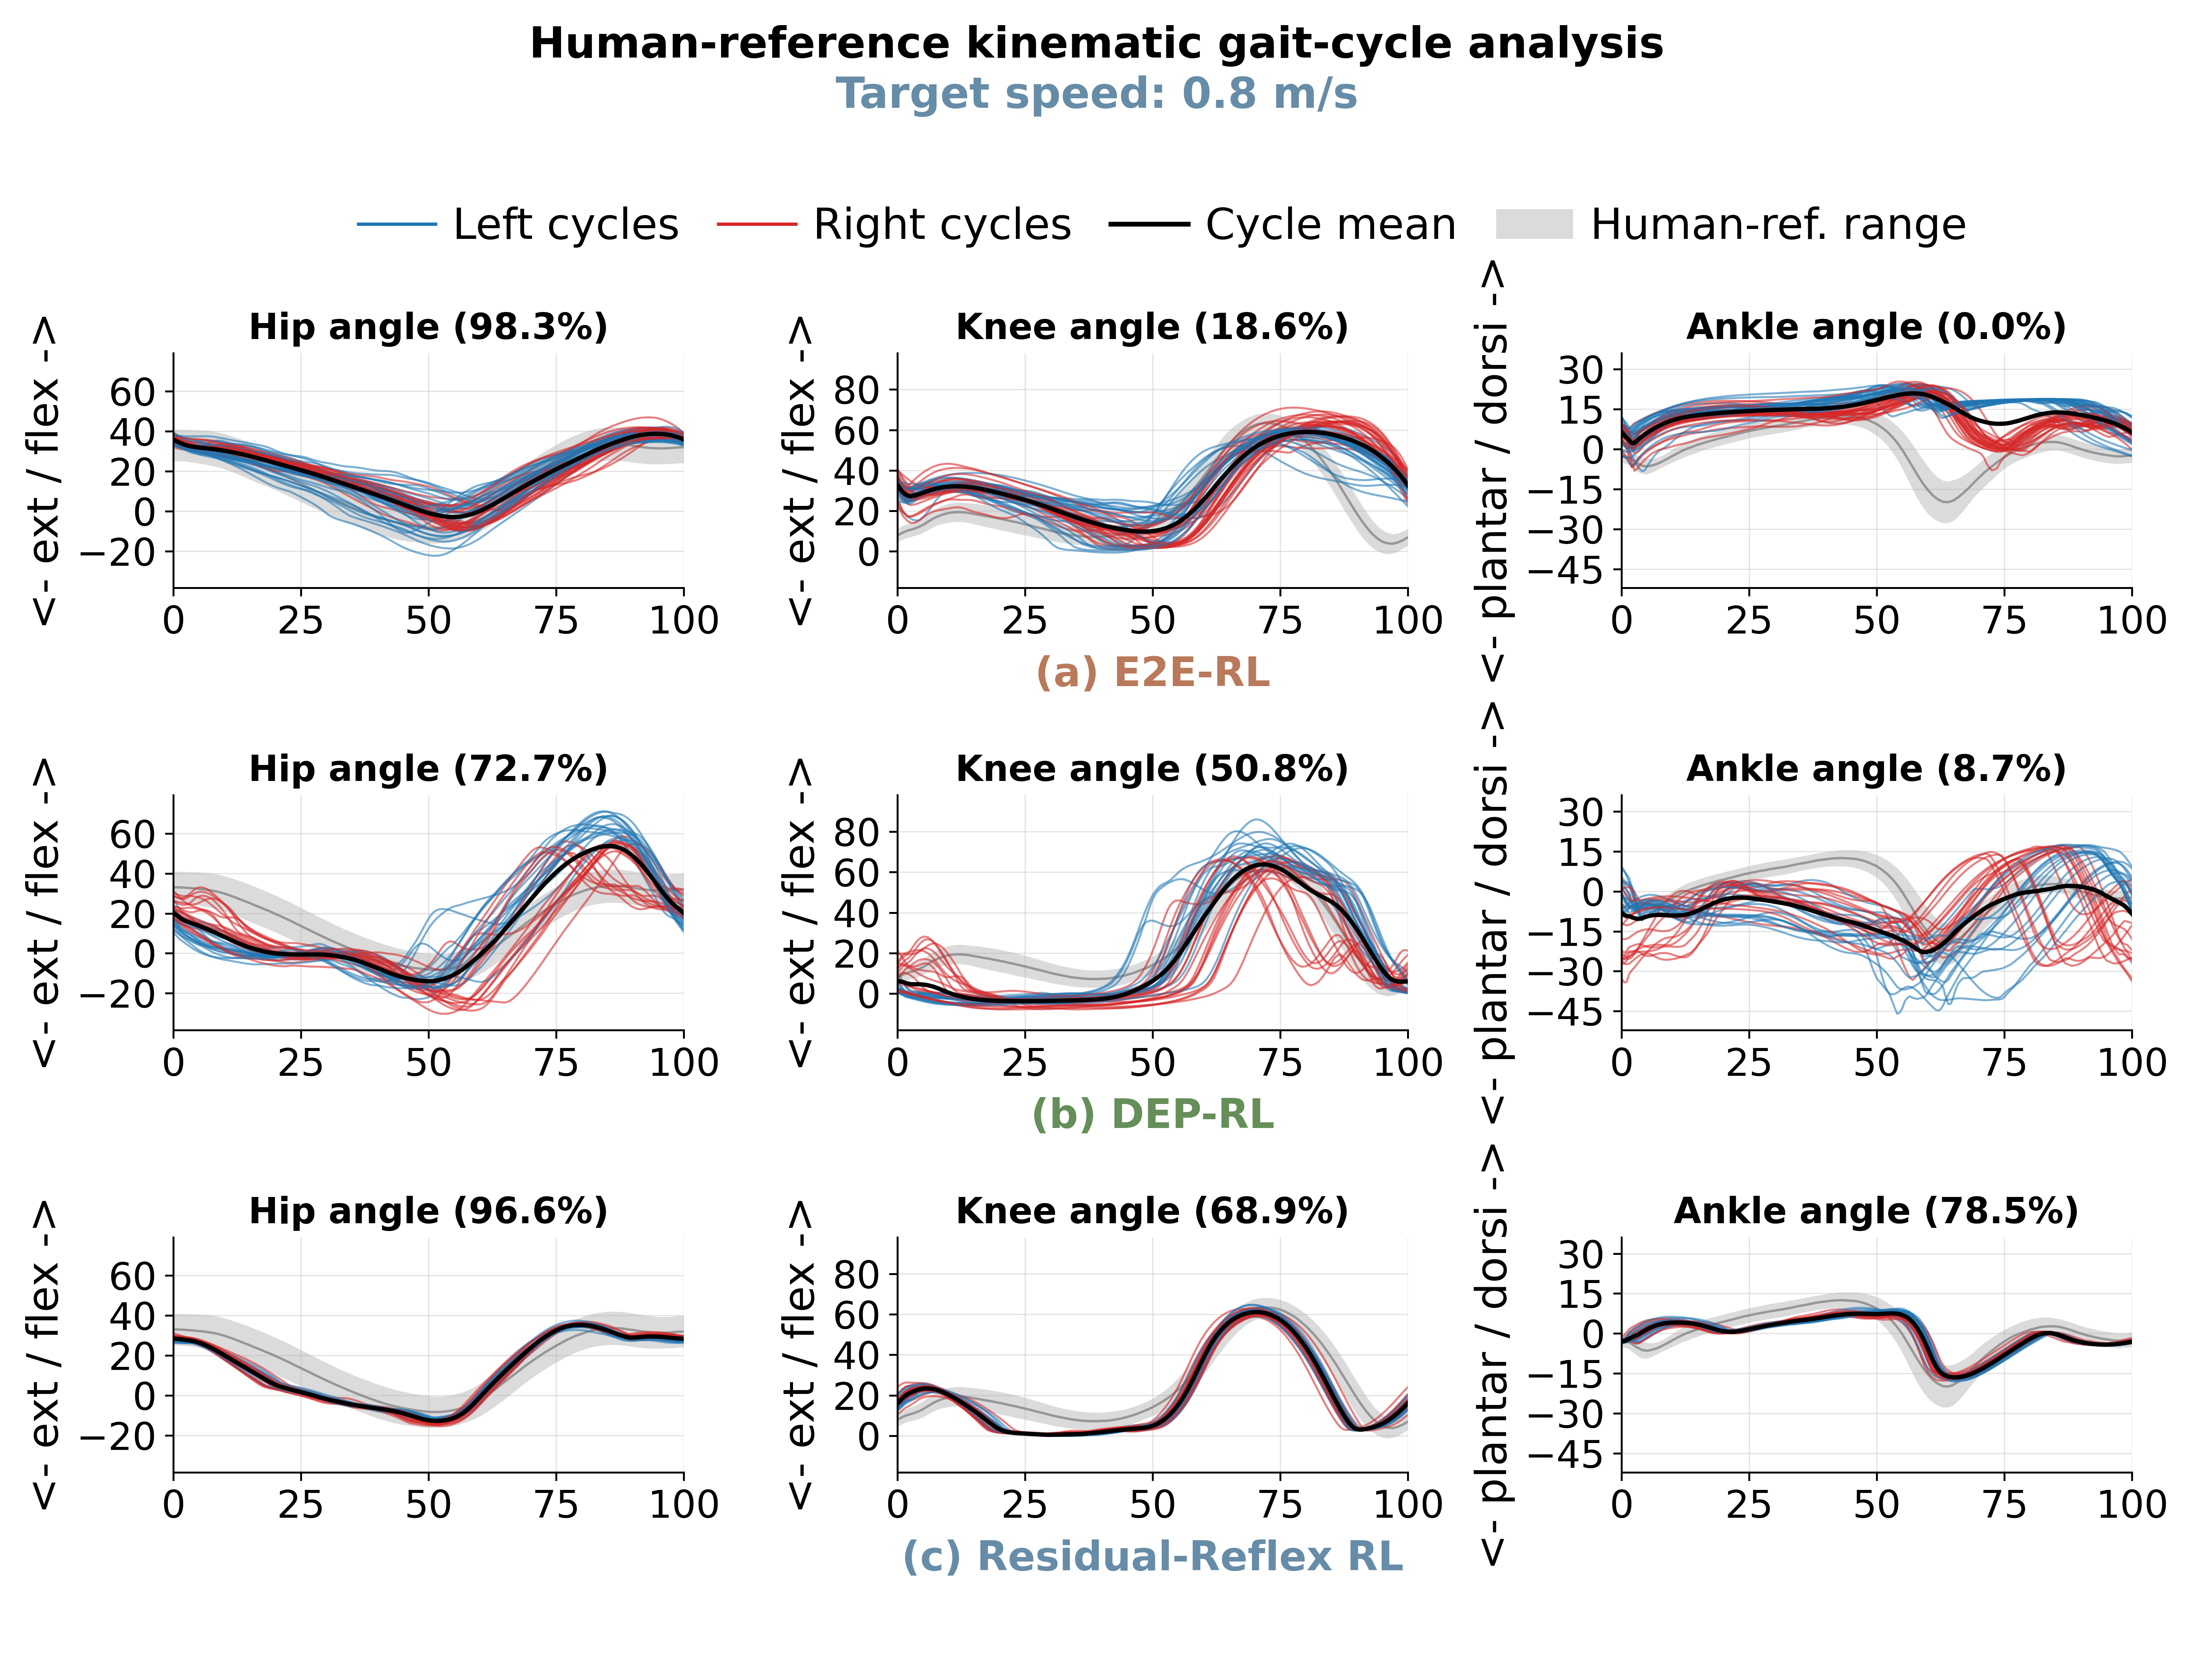
\includegraphics[width=\columnwidth]{gait_analysis_residual_vs_e2e_0p8.png}}
\caption{Human-reference kinematic gait-cycle visualization at target speed
\textbf{0.8~m/s} for E2E-RL, DEP-RL, and Residual-Reflex RL. Blue and red
curves denote left and right gait cycles, respectively; the black curve is the
cycle average and the gray band is the human-reference range. Horizontal axes
show normalized gait cycle percentage.}
\Description{Hip, knee, and ankle gait-cycle curves for three controllers at
0.8 meters per second are compared with human-reference ranges.}
\label{fig:gait_profiles_08}
\end{figure}

\begin{figure}[!t]
\centerline{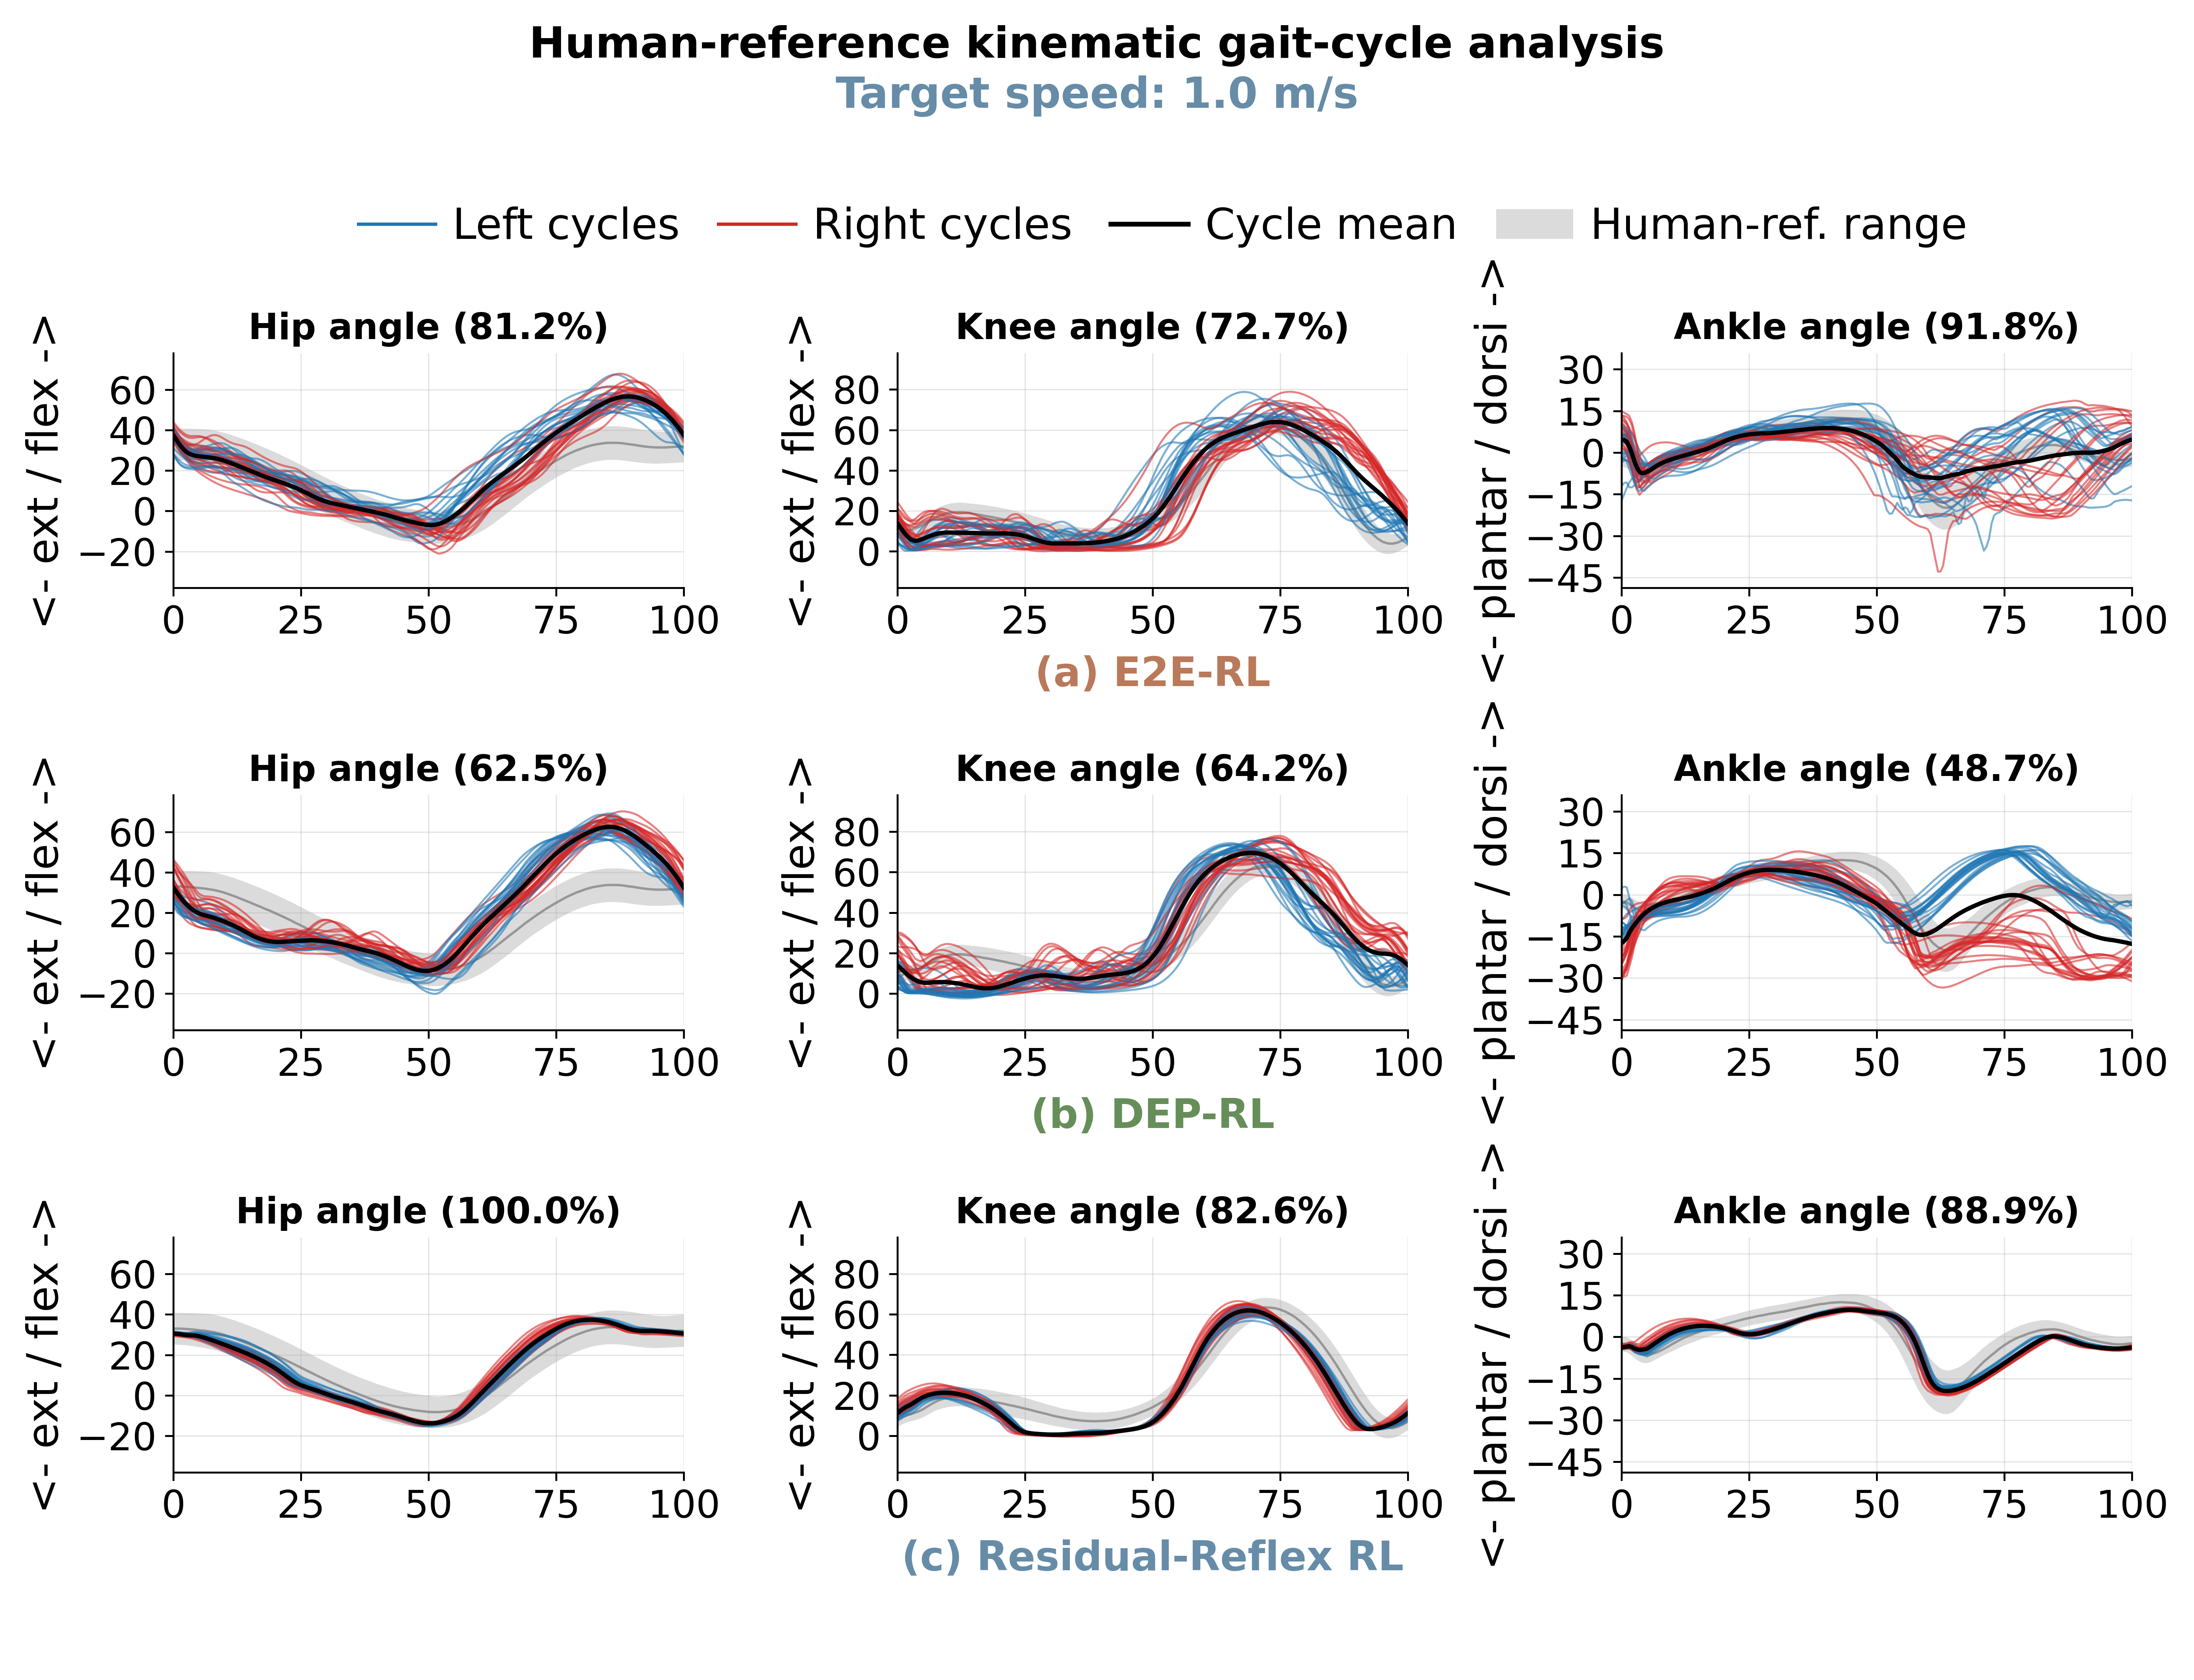
\includegraphics[width=\columnwidth]{gait_analysis_residual_vs_e2e_1p0.png}}
\caption{Human-reference kinematic gait-cycle visualization at target speed
\textbf{1.0~m/s} for E2E-RL, DEP-RL, and Residual-Reflex RL. Blue and red
curves denote left and right gait cycles, respectively; the black curve is the
cycle average and the gray band is the human-reference range. Horizontal axes
show normalized gait cycle percentage.}
\Description{Hip, knee, and ankle gait-cycle curves for three controllers at
1.0 meter per second are compared with human-reference ranges.}
\label{fig:gait_profiles_10}
\end{figure}

\begin{figure}[!t]
\centerline{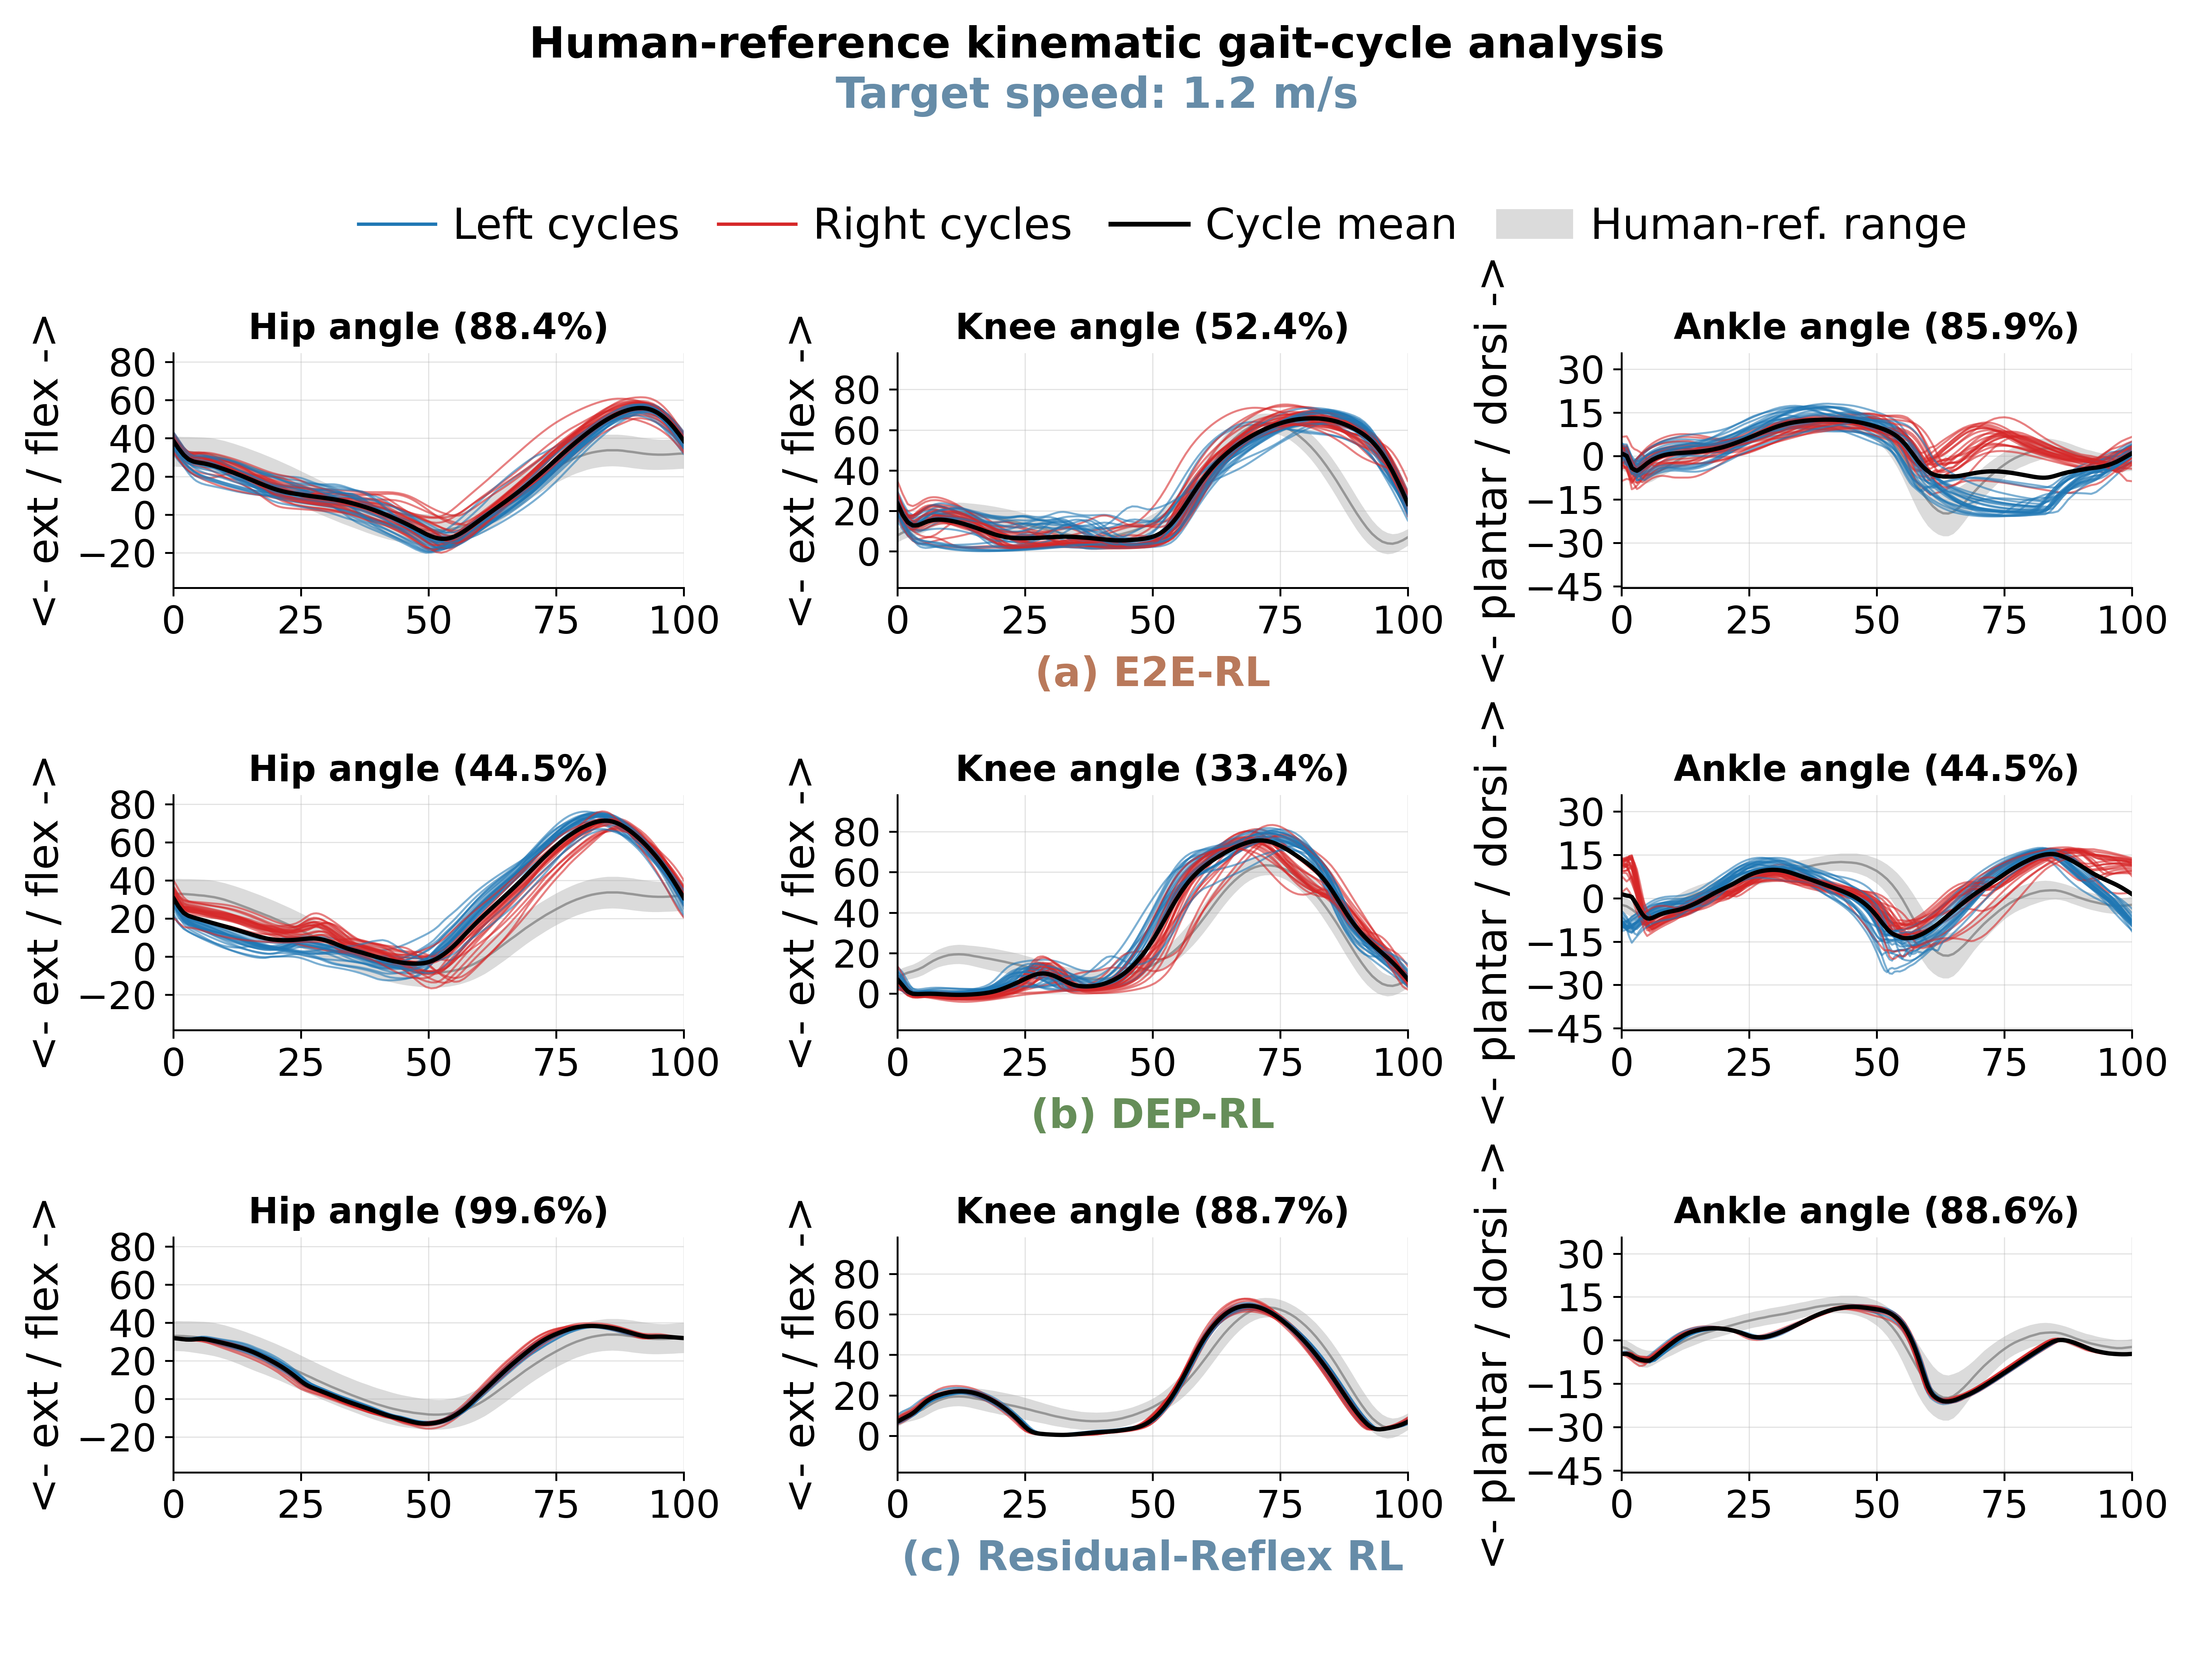
\includegraphics[width=\columnwidth]{gait_analysis_residual_vs_e2e_1p2.png}}
\caption{Human-reference kinematic gait-cycle visualization at target speed
\textbf{1.2~m/s} for E2E-RL, DEP-RL, and Residual-Reflex RL. Blue and red
curves denote left and right gait cycles, respectively; the black curve is the
cycle average and the gray band is the human-reference range. Horizontal axes
show normalized gait cycle percentage.}
\Description{Hip, knee, and ankle gait-cycle curves for three controllers at
1.2 meters per second are compared with human-reference ranges.}
\label{fig:gait_profiles_12}
\end{figure}

\subsubsection{Dynamic Plausibility}
The vertical GRF scores further distinguish the three controllers. As summarized in Table~\ref{tab:grf_scores}, Residual-Reflex RL consistently achieved the highest vertical GRF scores across all target walking speeds, indicating the closest agreement with the human-reference loading patterns. In contrast, both E2E-RL and DEP-RL produced substantially lower GRF morphology scores, with DEP-RL showing near-zero agreement at 1.0 and 1.2 m/s.

The corresponding GRF waveforms are shown in Fig.~\ref{fig:grf_morphology}. Residual-Reflex RL generated smoother vertical GRF profiles with a more human-reference double-support pattern throughout stance. In contrast, E2E-RL exhibited irregular loading despite producing visually plausible joint trajectories in some cases, whereas DEP-RL produced pronounced early-stance impact peaks and larger stride-to-stride variations, particularly at higher walking speeds.

A GRF score of 0 indicates that the averaged force profile remains outside the human-reference range after normalization, rather than reflecting only localized deviations. This observation highlights an important distinction between kinematic and dynamic evaluation. Although E2E-RL and DEP-RL can generate visually plausible joint motion, their foot–ground interactions remain substantially less consistent with human walking dynamics. The smoother GRF profiles produced by Residual-Reflex RL therefore demonstrate that the proposed controller improves not only joint kinematics but also dynamic consistency during stance.

\begin{table}[!t]
\centering
\caption{Vertical GRF human-reference scores in controlled walking validation.
Higher values indicate closer agreement with the human-reference vertical GRF
range.}
\label{tab:grf_scores}
\small
\setlength{\tabcolsep}{4pt}
\renewcommand{\arraystretch}{1.12}
\begin{tabular*}{\columnwidth}{@{\extracolsep{\fill}}l r r r}
\toprule
\textbf{Method} & \textbf{0.8~m/s} & \textbf{1.0~m/s} & \textbf{1.2~m/s} \\
\midrule
E2E-RL & 35.9 & 27.6 & 21.5 \\
DEP-RL & 39.8 & 0.0 & 0.0 \\
\textbf{Residual-Reflex RL} & \textbf{76.7} & \textbf{89.8} & \textbf{89.1} \\
\bottomrule
\end{tabular*}
\end{table}

\begin{figure}[!t]
\centerline{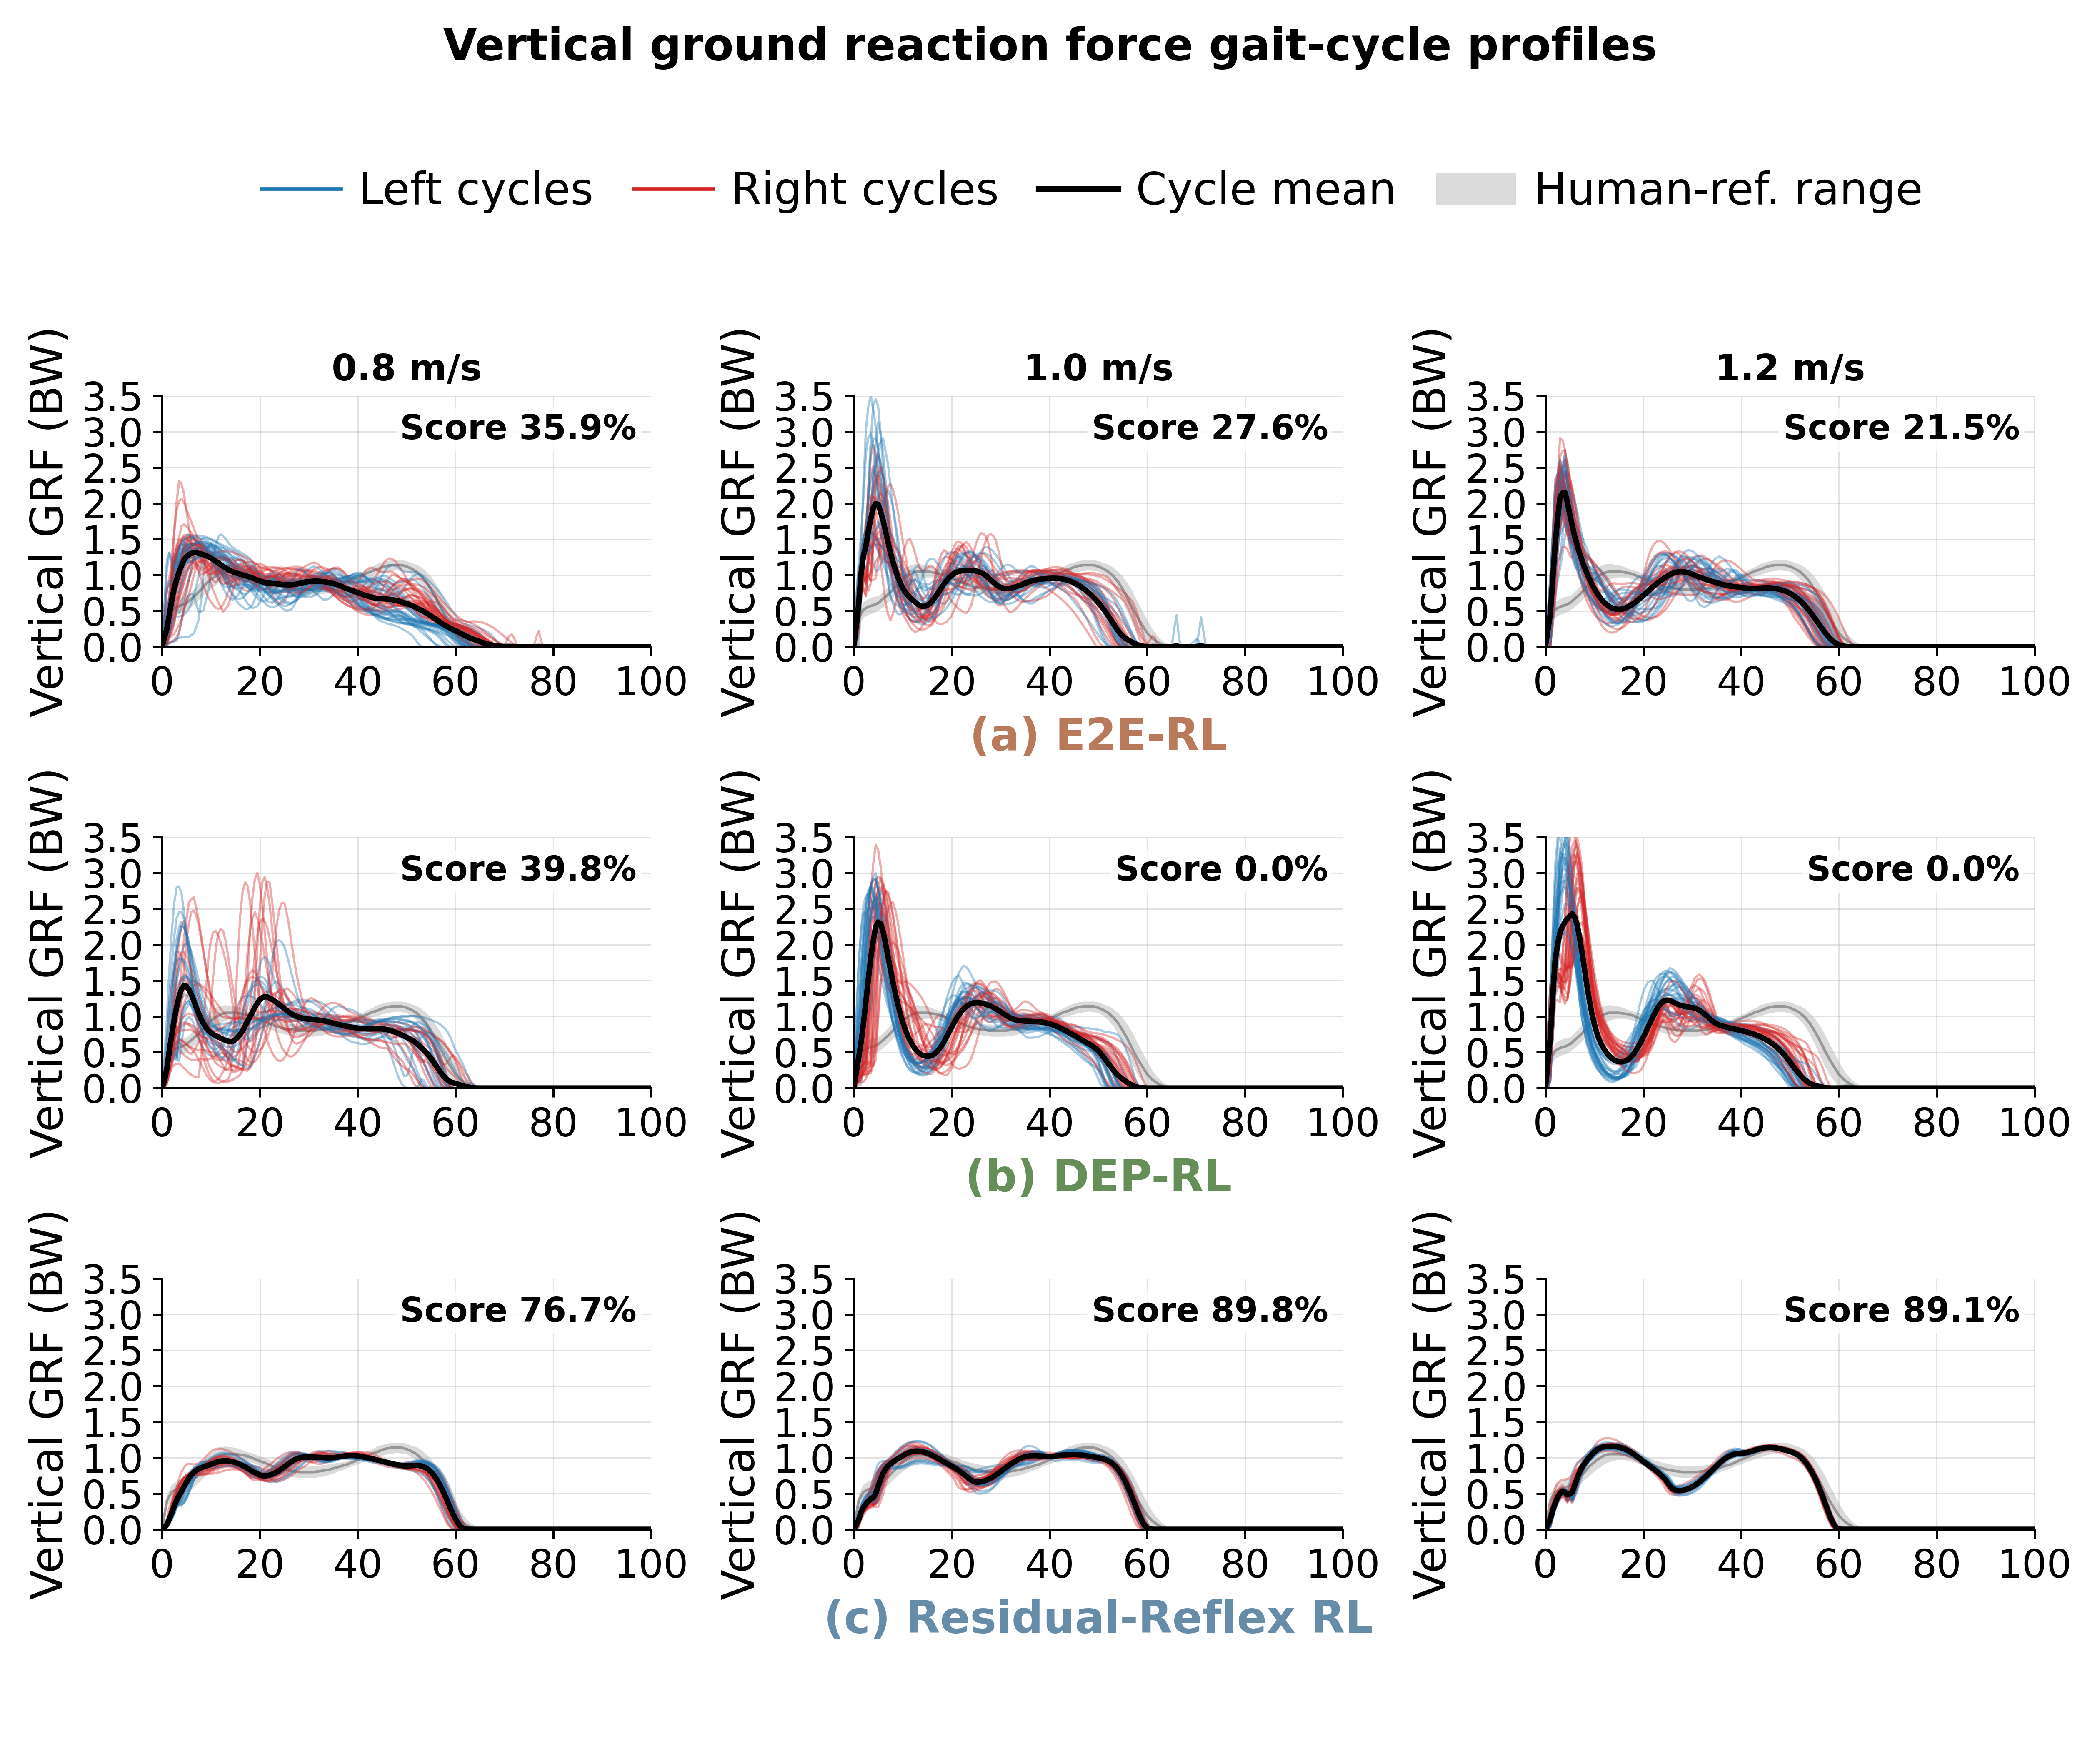
\includegraphics[width=\columnwidth]{grf_morphology_comparison.png}}
\caption{Vertical GRF morphology across target speeds for E2E-RL, DEP-RL, and
Residual-Reflex RL. Blue and red thin curves show individual left
and right normalized gait cycles, respectively; the black curve denotes the
cycle mean, the gray band denotes the human-reference range used for post-hoc
evaluation, and the panel annotations report the GRF human-reference score.
Horizontal axes show normalized gait cycle percentage.}
\Description{A grid compares left and right vertical ground-reaction-force
cycles for three controllers and three target speeds with human-reference
ranges. Residual-Reflex RL produces the most concentrated curves.}
\label{fig:grf_morphology}
\end{figure}

\subsubsection{Gait Consistency}
The symmetry and repeatability scores demonstrate that Residual-Reflex RL consistently produces more symmetric and repeatable gait cycles than E2E-RL and DEP-RL. As summarized in Table~\ref{tab:symmetry_variability}, Residual-Reflex RL achieved lower left–right waveform differences and lower stride time and stride length coefficients of variation across all target walking speeds. The Hip, Knee, Ankle, and GRF columns report the left–right waveform difference $D_y$, whereas the Time CV and Length CV columns report the coefficient of variation of stride time and stride length, respectively. The largest improvements are observed in ankle symmetry and stride variability, where E2E-RL and DEP-RL exhibit substantially less repeatable gait cycles.

These quantitative results are consistent with the waveform visualizations, indicating that residual-reflex modulation improves bilateral coordination as well as stride-to-stride repeatability. For example, at 1.2 m/s, Residual-Reflex RL achieved stride time and stride length coefficients of variation of only 0.70\% and 0.74\%, respectively, indicating that the standard deviations of these quantities were below 1\% of their corresponding mean values. In contrast, E2E-RL and DEP-RL exhibited considerably larger cycle-to-cycle variability.

These results indicate that the proposed controller not only produces a physiologically plausible average gait cycle, but also maintains consistent locomotion over successive steps.


\begin{table}[!t]
\centering
\caption{Cycle-level left--right waveform differences and stride variability.
Hip, knee, ankle, and GRF columns report $D_y$, the RMS difference between the
average left and right gait-cycle waveforms. Time CV and Length CV report
$100\sigma_z/\mu_z$ for stride time and stride length. Lower values indicate
more symmetric or more repeatable gait.}
\label{tab:symmetry_variability}
\small
\setlength{\tabcolsep}{3.5pt}
\renewcommand{\arraystretch}{1.12}
\resizebox{\columnwidth}{!}{%
\begin{tabular}{c l r r r r r r}
\toprule
\makecell{\textbf{Target}\\\textbf{speed}} & \textbf{Method} & \textbf{Hip} & \textbf{Knee} & \textbf{Ankle} & \textbf{GRF} & \makecell{\textbf{Time}\\\textbf{CV (\%)}} & \makecell{\textbf{Length}\\\textbf{CV (\%)}} \\
\midrule
\multirow[c]{3}{*}{0.8} & E2E-RL & 2.92 & 5.75 & 6.36 & 0.10 & 9.05 & 14.88 \\
 & DEP-RL & 11.20 & 11.73 & 11.59 & 0.12 & 7.96 & 11.04 \\
 & \textbf{Residual-Reflex RL} & \textbf{0.80} & \textbf{1.03} & \textbf{0.89} & \textbf{0.04} & \textbf{1.98} & \textbf{5.66} \\
\midrule
\multirow[c]{3}{*}{1.0} & E2E-RL & 6.12 & 10.61 & 6.69 & 0.07 & 5.03 & 5.63 \\
 & DEP-RL & 4.54 & 10.12 & 16.27 & 0.28 & 2.62 & 5.27 \\
 & \textbf{Residual-Reflex RL} & \textbf{1.78} & \textbf{1.85} & \textbf{0.97} & \textbf{0.03} & \textbf{1.51} & \textbf{1.86} \\
\midrule
\multirow[c]{3}{*}{1.2} & E2E-RL & 3.43 & 3.00 & 9.84 & 0.04 & 3.87 & 5.83 \\
 & DEP-RL & 8.33 & 5.83 & 6.31 & 0.34 & 2.29 & 4.78 \\
 & \textbf{Residual-Reflex RL} & \textbf{0.87} & \textbf{0.87} & \textbf{0.46} & \textbf{0.02} & \textbf{0.70} & \textbf{0.74} \\
\bottomrule
\end{tabular}%
}
\end{table}

\begin{figure}[!t]
\centerline{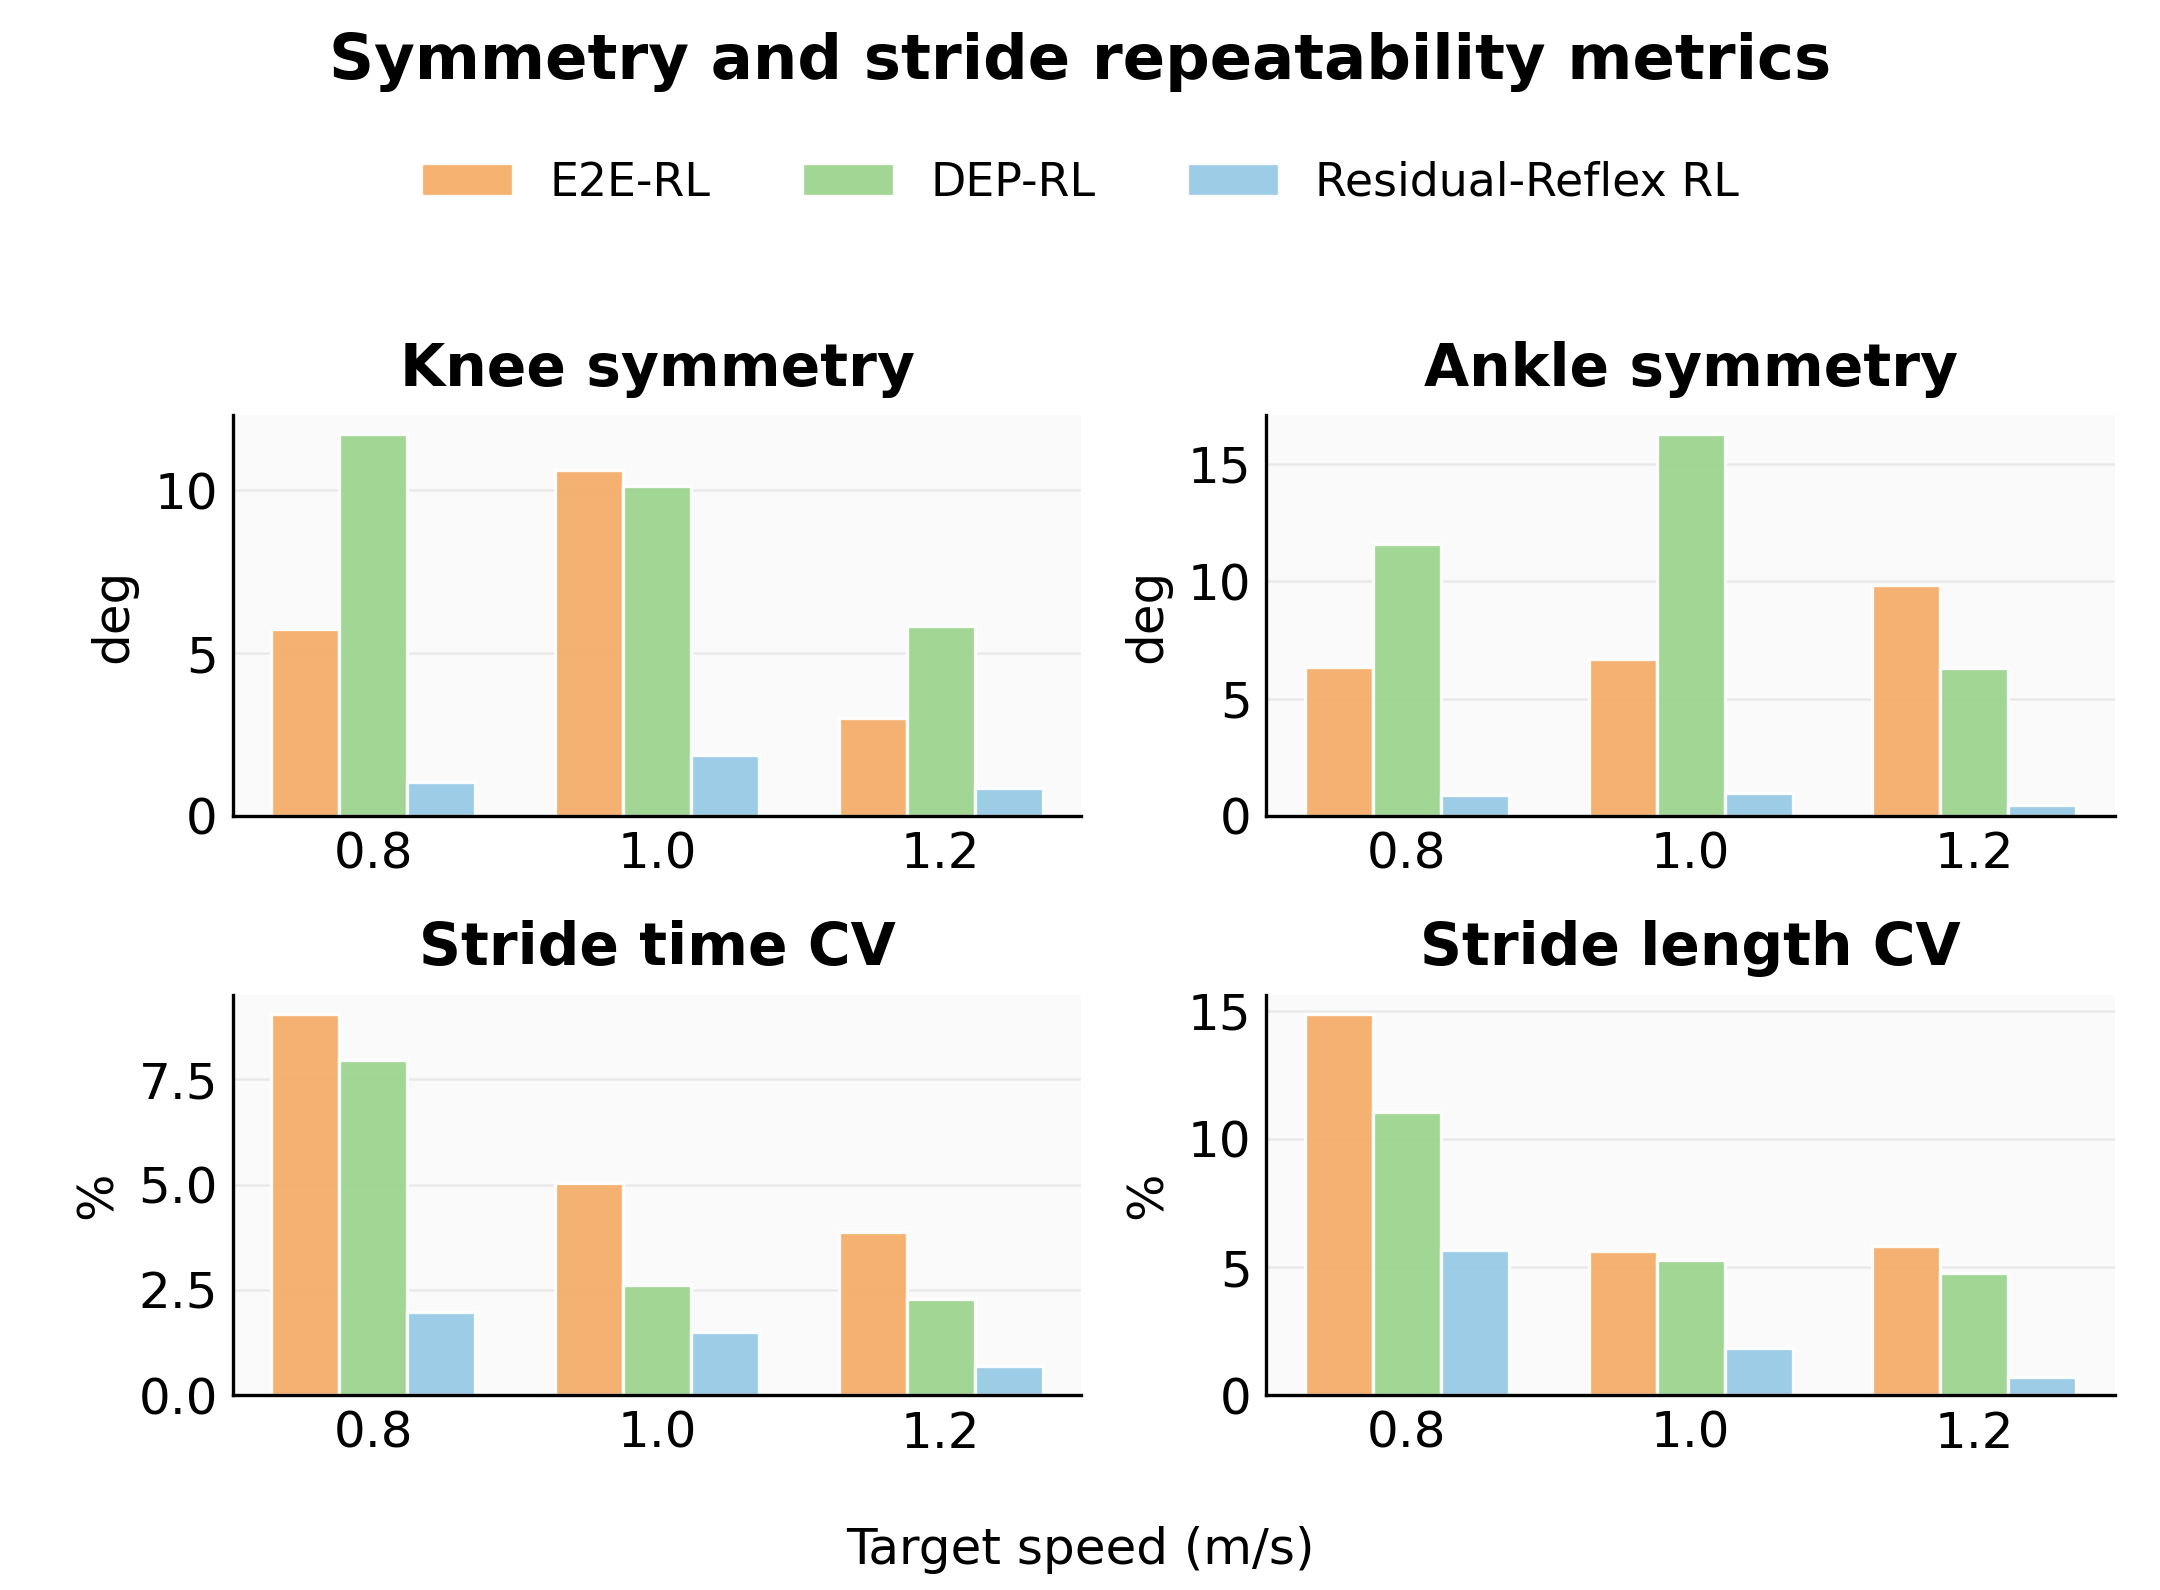
\includegraphics[width=\columnwidth]{gait_symmetry_variability_bars.png}}
\caption{Left--right waveform differences and stride variability across target
speeds. Lower values indicate more symmetric and more repeatable gait cycles.}
\Description{Bar charts compare bilateral waveform differences and stride
variability. Residual-Reflex RL generally has the lowest values.}
\label{fig:symmetry_variability_bars}
\end{figure}

\subsubsection{Qualitative Motion Analysis}
The qualitative gait snapshots in Fig.~\ref{fig:qualitative_snapshots} provide a visual interpretation of the quantitative results presented in the preceding sections. Representative frames sampled at 0\%, 25\%, 50\%, 75\%, and 100\% of the gait cycle illustrate how the different controllers organize stance, push-off, and swing throughout a complete walking cycle.

Residual-Reflex RL produces the most natural-looking gait sequence. The body remains upright throughout the gait cycle, while the transition between stance and swing is smooth and well coordinated. These observations are consistent with its higher joint-kinematic, GRF, and gait-consistency scores, indicating that the proposed controller achieves both physiologically plausible joint motion and stable foot–ground interaction.

E2E-RL also generates sustained walking and maintains visually reasonable postures throughout the gait cycle. However, when interpreted together with the quantitative results, the motion exhibits less coordinated limb movement and less consistent weight transfer, explaining its lower GRF and gait-consistency scores despite relatively good joint-kinematic performance in some conditions.

DEP-RL exhibits the largest qualitative deviations. Around 25\% of the gait cycle, the body leans further forward while the swing leg adopts a less natural knee–ankle configuration. Similar deviations remain visible near 75\% of the gait cycle, resulting in less coordinated stance-to-swing transitions. These observations are consistent with its lower joint-kinematic, GRF, and gait-consistency scores.

The accompanying \suppvideo{} further illustrates these differences over continuous motion. Compared with the sampled snapshots, the video more clearly reveals the temporal characteristics of weight transfer, limb coordination, and stride-to-stride consistency throughout the gait cycle.



\begin{figure}[!t]
\centerline{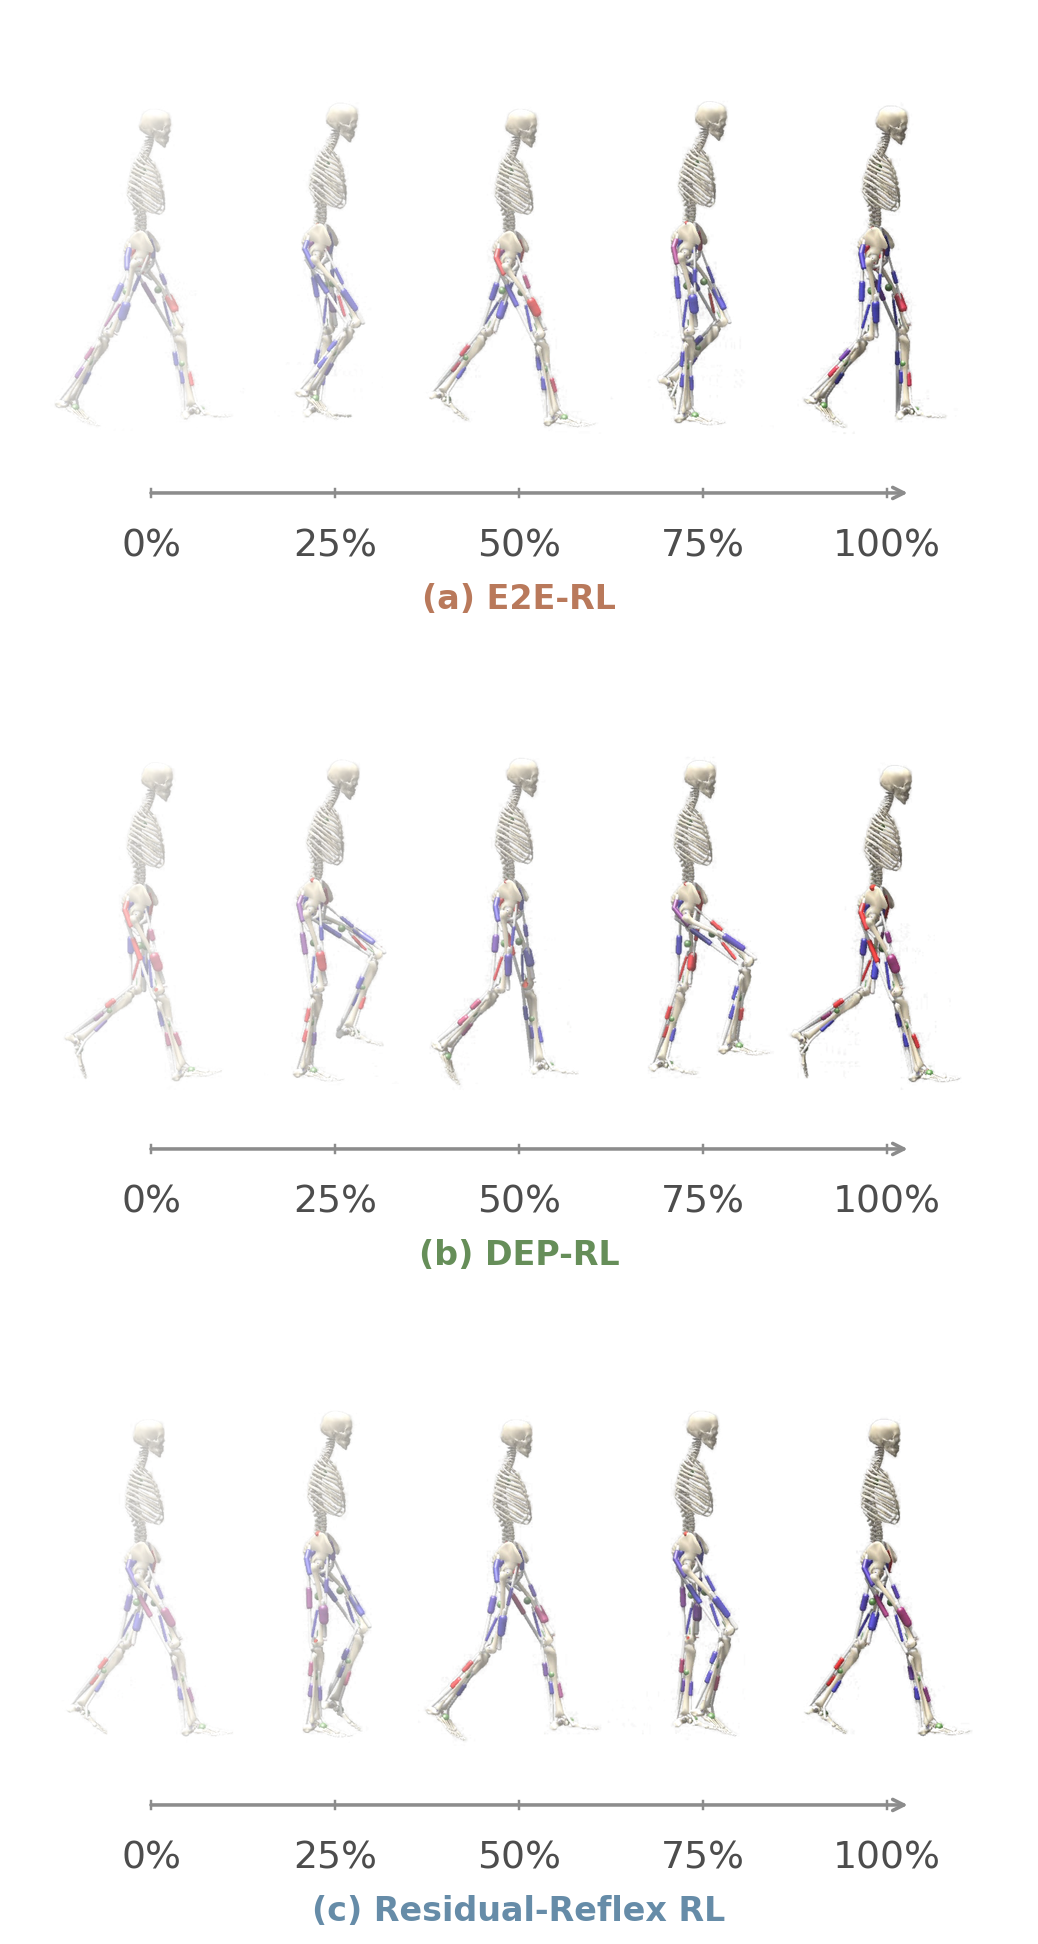
\includegraphics[width=1\columnwidth]{qualitative_gait_snapshots_1p2_one_cycle.png}}
\caption{Qualitative gait snapshots over one detected gait cycle at 1.2~m/s
for (a) E2E-RL, (b) DEP-RL, and (c) Residual-Reflex RL. Within each panel,
frames were sampled at 0\%, 25\%, 50\%, 75\%, and 100\% of the gait cycle
detected from the corresponding STO trajectory and synchronized video.}
\Description{Five gait phases for each controller show posture progression
through one walking cycle.}
\label{fig:qualitative_snapshots}
\end{figure}

\subsection{Adaptation to Plantarflexor Weakness}
\label{sec:weakness-adaptation}
Beyond nominal walking, this experiment evaluates whether the trained Residual-Reflex RL controller adapts to changes in musculoskeletal capacity without retraining. Plantarflexor weakness was simulated by reducing the maximum isometric force of the soleus muscles while keeping the trained 1.2 m/s policy fixed. Soleus strength was varied from 83\% to 100\% of the nominal value. Residual-Reflex RL was compared with the CMA-ES-optimized reflex controller under the same weakened musculoskeletal models. To analyze the adaptation strategy, we additionally report the root-mean-square (RMS) magnitude of each residual-action channel,

\begin{equation}
A_i^{\mathrm{RMS}} =
\sqrt{\frac{1}{T}\sum_{t=1}^{T}a_i(t)^2},
\end{equation}
where $a_i(t)$ is the $i$th residual action and $T$ is the number of evaluated policy steps. The RMS magnitude quantifies how strongly each residual channel is utilized regardless of sign.

\subsubsection{Survival comparison}
The survival results immediately distinguish the two controllers. As summarized in Table~\ref{tab:weakness_survival}, Residual-Reflex RL completed the full 25 s evaluation at all tested weakness levels, whereas the CMA-ES-optimized reflex controller terminated early for every weakened model and remained stable only under the nominal condition. These results demonstrate that online residual-reflex modulation substantially improves robustness to changes in musculoskeletal capacity compared with fixed offline-optimized reflex parameters.

\subsubsection{Speed adaptation analysis}
The speed adaptation results further reveal how the learned controller responds to reduced plantarflexor capacity. As shown in
Table~\ref{tab:weakness_adaptation} and
Fig.~\ref{fig:weakness_speed_adaptation}, the realized walking speed decreased gradually from 1.20 m/s under the nominal model to 0.95 m/s at 83\% soleus strength. Rather than maintaining the commanded speed at the expense of stability, the controller adopted a slower but stable gait as muscle capacity decreased. This behavior resembles a common compensatory strategy observed in human walking, where reduced plantarflexor strength is accompanied by a reduction in preferred walking speed. Importantly, the slower gait was not merely a degraded survival behavior. As shown in Fig.~\ref{fig:weakness_kinematic_profiles}, the generated joint trajectories remained close to the human-reference profiles across all tested weakness levels, yielding a joint-kinematic score of 89.0\% even at 83\% soleus strength. These results demonstrate that the proposed controller accommodates substantial changes in muscle capacity while preserving physiologically plausible locomotion without retraining.

The accompanying \suppvideo{} further illustrates the representative 83\% weakness condition. Residual-Reflex RL maintains a recognizable stance--swing sequence and upright progression, whereas the CMA-ES-optimized reflex controller loses balance and terminates. The synchronized gait-cycle curves further show the evolution of the hip, knee, ankle, and vertical GRF profiles during the two rollouts.

\subsubsection{Residual-action analysis}
The residual-action RMS values further explain the adaptation strategy adopted by the learned controller. Channel definitions are given in Table~\ref{tab:residual_actions}. Here we focus on how their modulation changes with soleus capacity. The soleus-related channel $a_3$ exhibits the largest RMS magnitude throughout the tested weakness range, indicating that ankle support and propulsion remain strongly regulated as plantarflexor capacity decreases. The policy does not compensate by monotonically increasing $a_3$. Instead, it accepts a lower walking speed while redistributing modulation across the remaining pathways. The stronger response of $a_4$ under greater weakness is consistent with increased reliance on knee-extension support when ankle push-off capacity is reduced, whereas $a_1$ and $a_2$ change more gradually. Together, the paired trends of ($a_1$,$a_2$) and ($a_3$,$a_4$) indicate coordinated redistribution across swing-related and stance-support pathways rather than single-parameter compensation. These results demonstrate that the four-dimensional residual action provides a compact adaptive interface for online neuromuscular regulation, enabling the same trained policy to generalize across weakened musculoskeletal models without retraining.


\begin{table}[!t]
\centering
\caption{Survival comparison under soleus weakness. Full episode duration is
25~s. The CMA-ES-optimized reflex controller remains stable only in the nominal
100\% model, whereas Residual-Reflex RL completes the episode across all tested
weakness levels without retraining.}
\label{tab:weakness_survival}
\small
\setlength{\tabcolsep}{1.8pt}
\renewcommand{\arraystretch}{1.1}
\begin{tabular*}{\columnwidth}{@{\extracolsep{\fill}}c c c c c}
\toprule
\textbf{Soleus} &
\makecell{\textbf{Residual}\\\textbf{duration}\\\textbf{(s)}} &
\makecell{\textbf{Residual}\\\textbf{full}} &
\makecell{\textbf{CMA-ES}\\\textbf{duration}\\\textbf{(s)}} &
\makecell{\textbf{CMA-ES}\\\textbf{full}} \\
\midrule
83\%  & 25.0 & Yes & 1.27 & No \\
87\%  & 25.0 & Yes & 1.28 & No \\
90\%  & 25.0 & Yes & 1.28 & No \\
93\%  & 25.0 & Yes & 1.29 & No \\
95\%  & 25.0 & Yes & 1.48 & No \\
97\%  & 25.0 & Yes & 1.47 & No \\
100\% & 25.0 & Yes & 25.0 & Yes \\
\bottomrule
\end{tabular*}
\end{table}

\begin{table}[!t]
\centering
\caption{Residual-Reflex RL under soleus weakness. The target speed was
1.2~m/s. All listed residual rollouts reached 1000 steps. Channel $a_3$ is the
soleus force-feedback modulation defined in Table~\ref{tab:residual_actions}.}
\label{tab:weakness_adaptation}
\small
\setlength{\tabcolsep}{4pt}
\renewcommand{\arraystretch}{1.1}
\begin{tabular*}{\columnwidth}{@{\extracolsep{\fill}}c c c c}
\toprule
\makecell{\textbf{Soleus}\\\textbf{strength}} &
\makecell{\textbf{Realized speed}\\\textbf{(m/s)}} &
\makecell{\textbf{Speed error}\\\textbf{(m/s)}} &
\textbf{RMS $\boldsymbol{a_3}$} \\
\midrule
83\%  & 0.949 & 0.251 & \textbf{0.846} \\
87\%  & 1.002 & 0.198 & \textbf{0.851} \\
90\%  & 1.063 & 0.137 & \textbf{0.878} \\
93\%  & 1.112 & 0.088 & \textbf{0.885} \\
95\%  & 1.137 & 0.063 & \textbf{0.889} \\
97\%  & 1.167 & 0.033 & \textbf{0.895} \\
100\% & 1.201 & 0.001 & \textbf{0.898} \\
\bottomrule
\end{tabular*}
\end{table}

\begin{figure}[!t]
\centerline{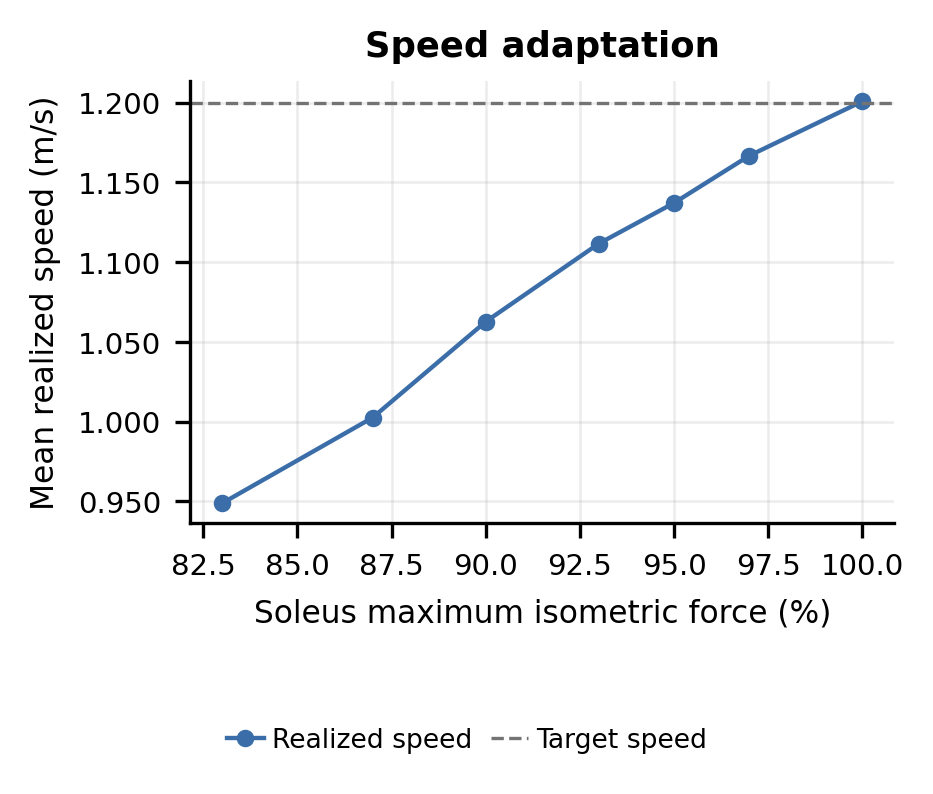
\includegraphics[width=0.78\columnwidth]{weakness_speed_adaptation.png}}
\caption{Speed adaptation under plantarflexor weakness. The same trained
Residual-Reflex RL policy remains stable across weakened soleus models but
adopts a slower realized speed as force capacity is reduced.}
\Description{Realized speed decreases smoothly as soleus maximum isometric
force is reduced from 100 to 83 percent.}
\label{fig:weakness_speed_adaptation}
\end{figure}

\begin{figure}[!t]
\centerline{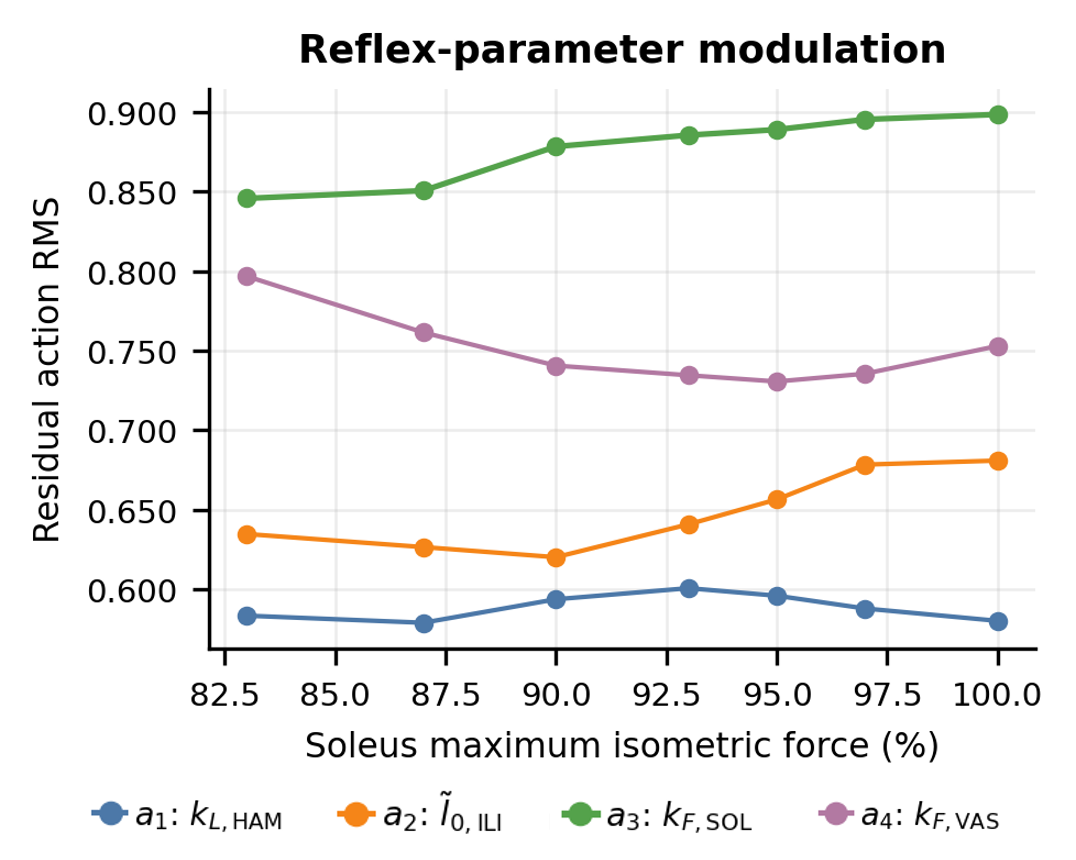
\includegraphics[width=0.78\columnwidth]{weakness_residual_action_rms.png}}
\caption{Residual-action modulation under plantarflexor weakness. RMS values
show that the trained policy continues to adjust all four selected reflex
channels. Channel $a_3$ modulates soleus force feedback for ankle
support/propulsion, whereas $a_4$ modulates vasti force feedback for knee
extension and stance support.}
\Description{Four curves show the root-mean-square magnitude of each residual
reflex action across soleus strength levels. The soleus-related third channel
has the largest magnitude.}
\label{fig:weakness_residual_action_rms}
\end{figure}

\begin{figure}[!t]
\centerline{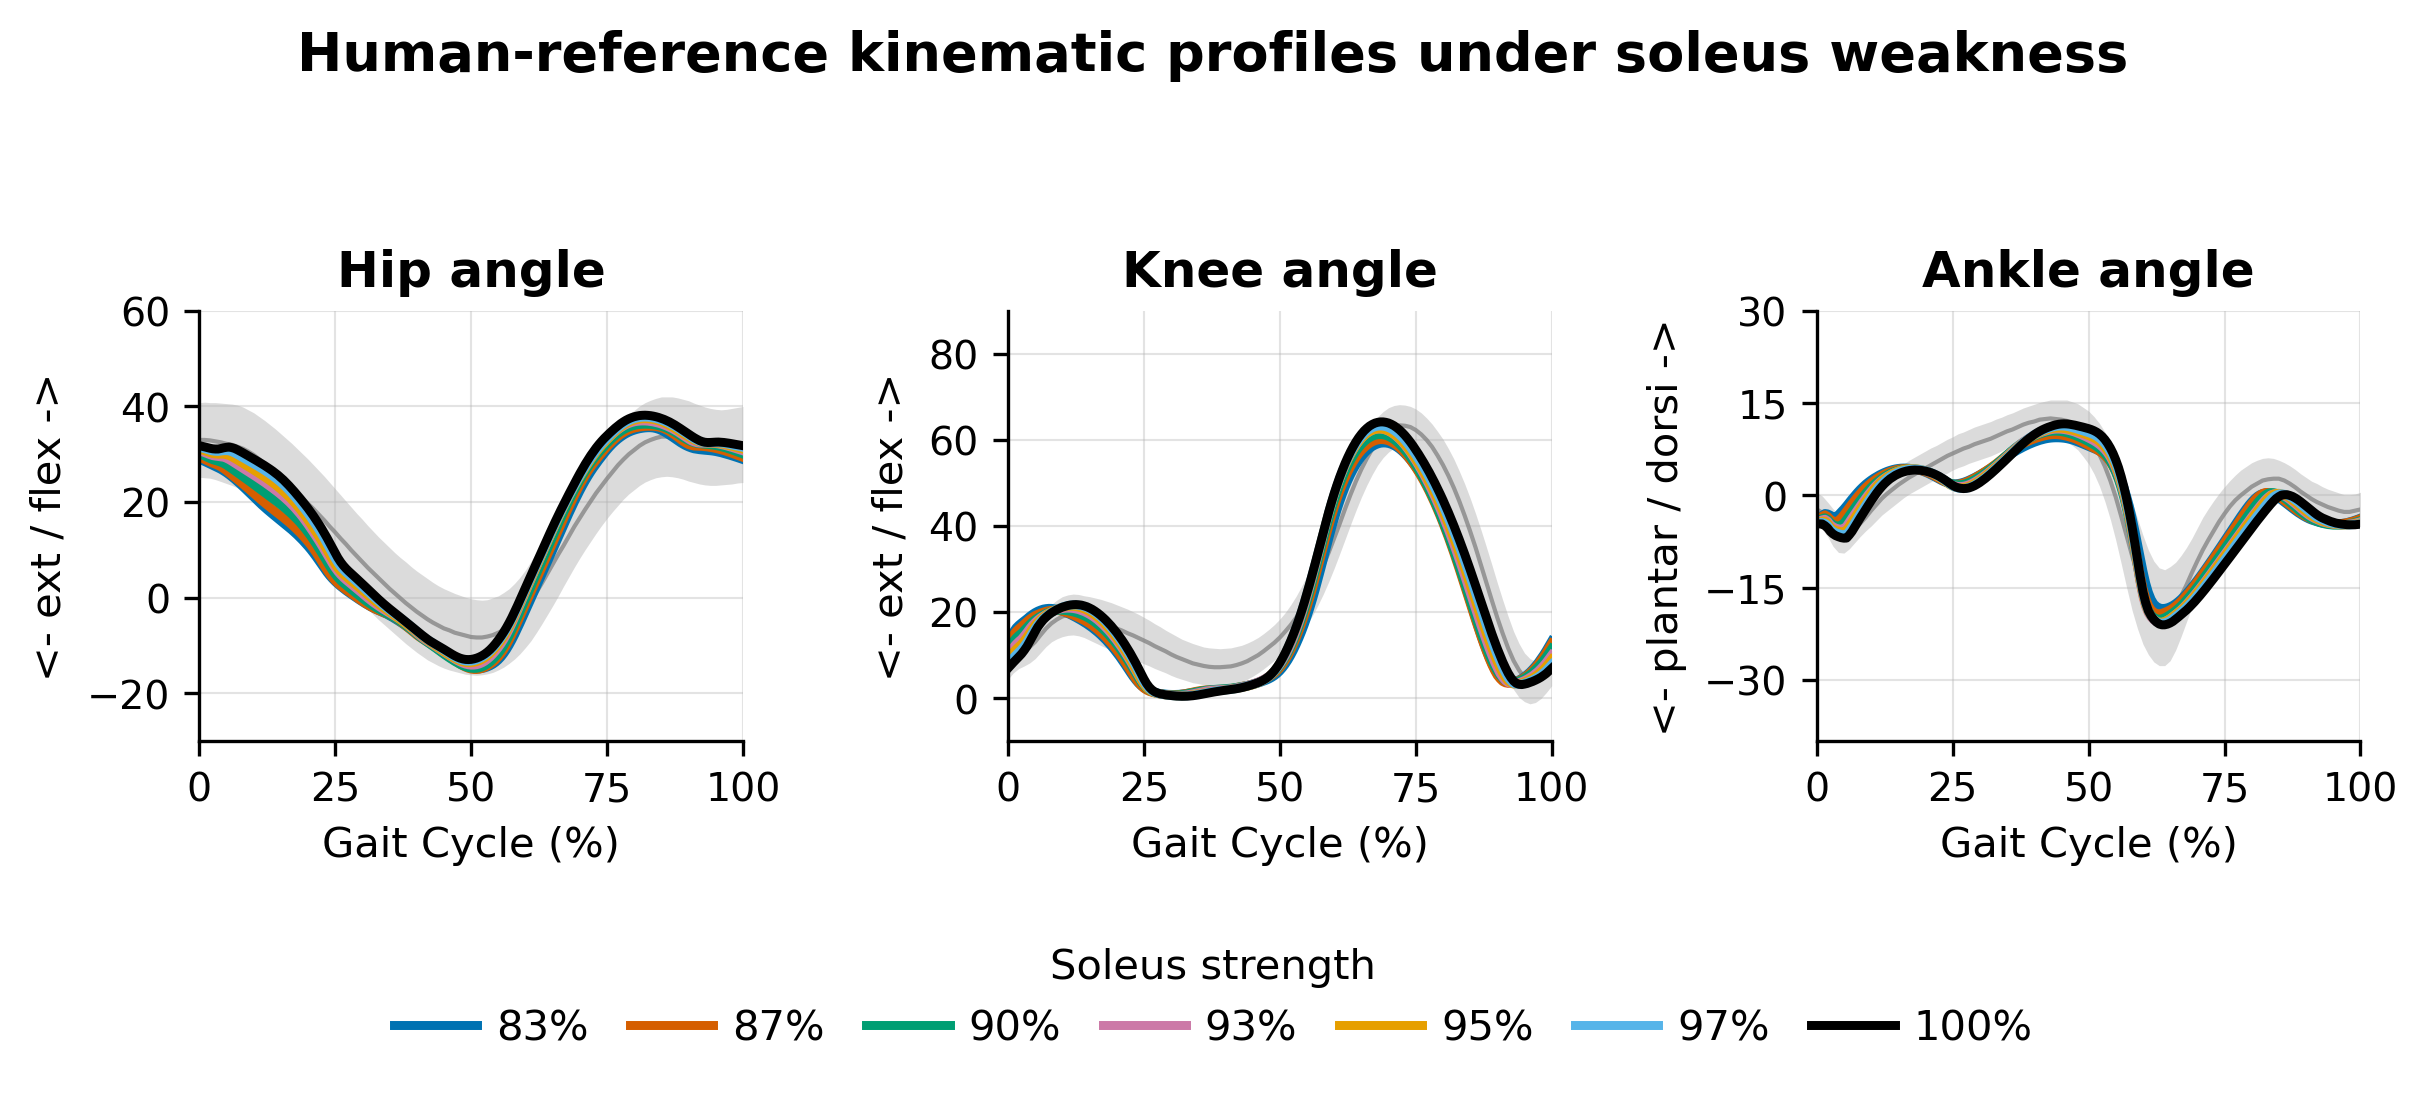
\includegraphics[width=\columnwidth]{weakness_kinematic_profiles.png}}
\caption{Human-reference kinematic profiles under soleus weakness. Colored
curves show the mean normalized gait-cycle profiles generated by the same
trained Residual-Reflex RL policy under different soleus strength levels; the
gray bands denote the human-reference ranges.}
\Description{Hip, knee, and ankle gait-cycle curves at seven soleus strength
levels remain near the human-reference ranges.}
\label{fig:weakness_kinematic_profiles}
\end{figure}

\subsection{Recovery from External Pushes}
\label{sec:push-recovery}
This experiment evaluates whether the trained Residual-Reflex RL controller can recover from external disturbances without retraining. The same 1.2 m/s policy used in the nominal walking and plantarflexor-weakness experiments was retained without further learning. Backward force pulses were applied to the torso for 0.1 s starting at 3.0 s. Perturbation magnitudes of 75 N and 100 N were evaluated under both single-push and repeated-push (every 5 s) conditions. Residual-Reflex RL was compared with the CMA-ES-optimized reflex controller under identical perturbation settings.

As summarized in Table~\ref{tab:push_perturbation}, Residual-Reflex RL successfully recovered from both 75 N and 100 N single backward pushes and maintained walking for the full 25 s evaluation. Under repeated perturbations, the controller also completed the full evaluation under the 75 N condition, whereas the more challenging 100 N repeated pushes resulted in termination after 20.1 s. In contrast, the CMA-ES-optimized reflex controller consistently failed after approximately 4.5–4.6 s under all perturbation conditions. These results demonstrate that the learned residual-reflex policy substantially improves recovery capability beyond fixed offline-optimized reflex gains.

Figure~\ref{fig:push_snapshots} provides a qualitative comparison of the recovery process under the representative 100 N single-push condition. Before the perturbation, both controllers produce stable walking. Following the force pulse, the CMA-ES-optimized reflex controller progressively loses balance and terminates, whereas Residual-Reflex RL reorganizes the subsequent steps, restores upright walking, and completes the full evaluation. The matched frames therefore distinguish sustained recovery from trajectories that merely delay failure.

The accompanying \suppvideo{} first illustrates the single-push recovery process by comparing Residual-Reflex RL under 75~N and 100~N backward pushes with the CMA-ES-optimized reflex controller under a 100~N backward push. Residual-Reflex RL reorganizes foot placement and resumes periodic walking after the disturbance, whereas the CMA-ES-optimized reflex controller fails to regain a stable gait. The video then compares Residual-Reflex RL under repeated 75~N and 100~N backward pushes applied every 5~s. The controller remains stable throughout the 75~N trial but terminates after 20.1~s under repeated 100~N pushes, illustrating the boundary of its recovery capability. Together with the plantarflexor-weakness experiments, these results demonstrate that residual-reflex modulation provides a flexible online adaptation mechanism for changes in both musculoskeletal capacity and external disturbances.

\begin{table}[!t]
\centering
\caption{External backward push perturbation results. Full episode duration is
25~s.}
\label{tab:push_perturbation}
\small
\setlength{\tabcolsep}{1.8pt}
\renewcommand{\arraystretch}{1.08}
\begin{tabular*}{\columnwidth}{@{\extracolsep{\fill}}c c c c c}
\toprule
\textbf{Method} & \textbf{Perturbation} & \makecell{\textbf{Force}\\\textbf{(N)}} &
\makecell{\textbf{Duration}\\\textbf{(s)}} &
\makecell{\textbf{Speed}\\\textbf{(m/s)}} \\
\midrule
\multirow[c]{4}{*}{\makecell[c]{Residual-\\Reflex RL}} &
\multirow{2}{*}{Single push} & 75  & 25.0 & 1.188 \\
& & 100 & 25.0 & 1.176 \\
\cmidrule(lr){2-5}
& \multirow{2}{*}{Every 5~s} & 75  & 25.0 & 1.129 \\
& & 100 & 20.1 & 1.091 \\
\midrule
\multirow[c]{4}{*}{\makecell[c]{CMA-ES-\\optimized\\Reflex}} &
\multirow{2}{*}{Single push} & 75  & 4.5 & 1.098 \\
& & 100 & 4.6 & 1.069 \\
\cmidrule(lr){2-5}
& \multirow{2}{*}{Every 5~s} & 75  & 4.5 & 1.098 \\
& & 100 & 4.6 & 1.069 \\
\bottomrule
\end{tabular*}
\end{table}

\begin{figure*}[!t]
\centering
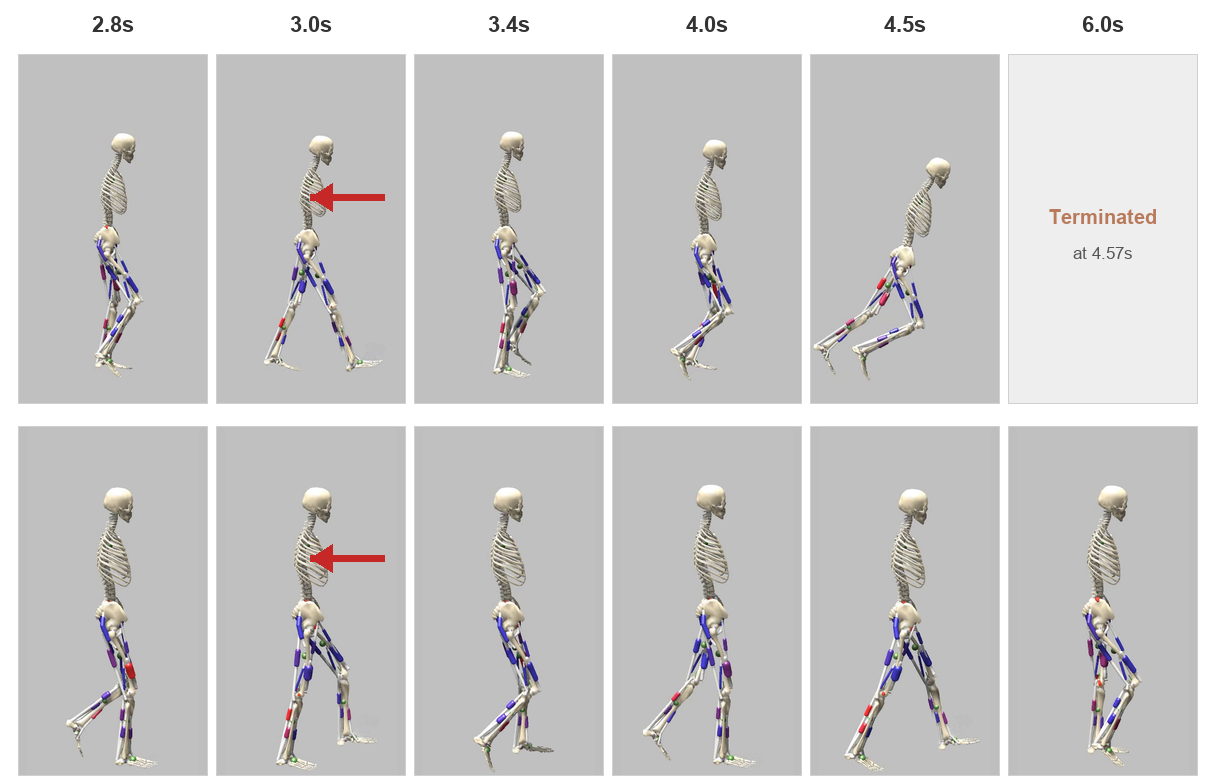
\includegraphics[width=0.94\textwidth]{push_perturbation_snapshots_100N.png}
\caption{Time-aligned response to a 100~N backward torso push applied for 0.1~s
at $t=3.0~\mathrm{s}$. Columns show synchronized frames from 2.8~s to 6.0~s. The
CMA-ES-optimized reflex controller (top) progressively loses upright balance
and terminates at 4.57~s. Residual-Reflex RL (bottom) modifies the following
steps and continues walking for the full 25~s rollout under the same
perturbation. Red arrows indicate the applied force.}
\Description{Two synchronized frame sequences compare recovery after a
backward torso push. The optimized reflex controller falls, whereas
Residual-Reflex RL reorganizes its steps and continues walking.}
\label{fig:push_snapshots}
\end{figure*}



\section{Discussion}
\label{sec:discussion}
The experimental results demonstrate that regulating an existing neuromuscular controller through reinforcement learning provides a practical way to improve both physiological plausibility and adaptability in muscle-driven locomotion. Under nominal walking conditions, Residual-Reflex RL consistently achieved better joint kinematics, more human-like ground reaction forces, and higher gait consistency than end-to-end muscle-control policies. The weakness and perturbation experiments further showed that the same trained policy remained effective under changes in musculoskeletal capacity and external disturbances without retraining. Together, these results indicate that reinforcement learning can benefit from regulating neuromuscular control mechanisms rather than directly generating muscle actions.

The observed improvements in joint kinematics, GRF morphology, and gait consistency can be understood from the learning formulation itself. In end-to-end muscle control, reinforcement learning directly operates in a high-dimensional and redundant muscle action space, where both muscle activation and the functional relationships among muscles must be learned from task rewards. In the proposed framework, the underlying neuromuscular topology is fixed by the phase-dependent reflex controller, such that the functional organization of sensory feedback pathways is explicitly defined. Reinforcement learning therefore no longer needs to construct this neuromuscular organization from scratch, but instead learns how to regulate a small set of biomechanically meaningful reflex parameters according to the current state. This allows learning to focus on state-dependent adaptation while preserving the existing neuromuscular organization.

The weakness and perturbation experiments further clarify why this formulation improves adaptability. The CMA-ES-optimized reflex controller also relies on physiological feedback, but its parameters remain fixed once optimization is completed. In contrast, Residual-Reflex RL preserves the same neuromuscular control structure while continuously adjusting the selected reflex parameters according to the current musculoskeletal state. This adaptation mechanism becomes particularly important when muscle capacity changes or external disturbances occur, because the controller can continuously regulate the underlying reflex parameters instead of relying on a single fixed parameter set. These findings demonstrate that reflex-informed neuromuscular regulation provides an effective formulation for improving both physiological plausibility and adaptability in muscle-driven locomotion.


\section{Conclusion}
We presented a Reflex-Informed Neuromuscular Reinforcement Learning framework for adaptive muscle-driven locomotion. Instead of directly generating muscle excitations, the proposed framework learns to regulate four biomechanically meaningful residual parameters of a phase-dependent reflex controller. This formulation preserves the underlying neuromuscular control structure while enabling reinforcement learning to adapt reflex behavior online through a compact and interpretable control interface.

Experiments in a Hyfydy-based musculoskeletal simulation demonstrated that the proposed framework consistently improved physiological plausibility under nominal walking conditions. Compared with end-to-end muscle-control policies, Residual-Reflex RL generated more human-like joint kinematics, ground reaction forces, and gait consistency across walking speeds of 0.8, 1.0, and 1.2~m/s. Beyond nominal walking, the same trained policy remained effective under plantarflexor weakness and external perturbations without retraining, demonstrating improved adaptability while preserving physiologically plausible locomotion.

These results demonstrate that integrating reinforcement learning with an existing neuromuscular control structure provides an effective formulation for simultaneously improving physiological plausibility and adaptability in muscle-driven locomotion. The proposed framework offers a compact and biologically meaningful learning interface that is applicable to muscle-driven character animation, computational studies of human locomotion, and bio-inspired locomotor control. Future work will extend the framework to continuous speed transitions, broader musculoskeletal morphologies, and more diverse physical interactions.

\FloatBarrier
\bibliographystyle{ACM-Reference-Format}
\bibliography{references}

\end{document}

%%
%% The "title" command has an optional parameter,
%% allowing the author to define a "short title" to be used in page headers.
\title{The Name of the Title Is Hope}

%%
%% The "author" command and its associated commands are used to define
%% the authors and their affiliations.
%% Of note is the shared affiliation of the first two authors, and the
%% "authornote" and "authornotemark" commands
%% used to denote shared contribution to the research.
\author{Ben Trovato}
\authornote{Both authors contributed equally to this research.}
\email{trovato@corporation.com}
\orcid{1234-5678-9012}
\author{G.K.M. Tobin}
\correspondingauthor
\authornotemark[1]
\email{webmaster@marysville-ohio.com}
\affiliation{%
  \institution{Institute for Clarity in Documentation}
  \city{Dublin}
  \state{Ohio}
  \country{USA}
}

\author{Lars Th{\o}rv{\"a}ld}
\affiliation{%
  \institution{The Th{\o}rv{\"a}ld Group}
  \city{Hekla}
  \country{Iceland}}
\email{larst@affiliation.org}

\author{Valerie B\'eranger}
\affiliation{%
  \institution{Inria Paris-Rocquencourt}
  \city{Rocquencourt}
  \country{France}
}

\author{Aparna Patel}
\affiliation{%
 \institution{Rajiv Gandhi University}
 \city{Doimukh}
 \state{Arunachal Pradesh}
 \country{India}}

\author{Huifen Chan}
\affiliation{%
  \institution{Tsinghua University}
  \city{Haidian Qu}
  \state{Beijing Shi}
  \country{China}}

\author{Charles Palmer}
\affiliation{%
  \institution{Palmer Research Laboratories}
  \city{San Antonio}
  \state{Texas}
  \country{USA}}
\email{cpalmer@prl.com}

\author{John Smith}
\affiliation{%
  \institution{The Th{\o}rv{\"a}ld Group}
  \city{Hekla}
  \country{Iceland}}
\email{jsmith@affiliation.org}

\author{Julius P. Kumquat}
\correspondingauthor
\affiliation{%
  \institution{The Kumquat Consortium}
  \city{New York}
  \country{USA}}
\email{jpkumquat@consortium.net}

%%
%% By default, the full list of authors will be used in the page
%% headers. Often, this list is too long, and will overlap
%% other information printed in the page headers. This command allows
%% the author to define a more concise list
%% of authors' names for this purpose.
\renewcommand{\shortauthors}{Trovato et al.}

%%
%% The abstract is a short summary of the work to be presented in the
%% article.
\begin{abstract}
  A clear and well-documented \LaTeX\ document is presented as an
  article formatted for publication by ACM in a conference proceedings
  or journal publication. Based on the ``acmart'' document class, this
  article presents and explains many of the common variations, as well
  as many of the formatting elements an author may use in the
  preparation of the documentation of their work.
\end{abstract}

%%
%% The code below is generated by the tool at http://dl.acm.org/ccs.cfm.
%% Please copy and paste the code instead of the example below.
%%
\begin{CCSXML}
<ccs2012>
 <concept>
  <concept_id>00000000.0000000.0000000</concept_id>
  <concept_desc>Do Not Use This Code, Generate the Correct Terms for Your Paper</concept_desc>
  <concept_significance>500</concept_significance>
 </concept>
 <concept>
  <concept_id>00000000.00000000.00000000</concept_id>
  <concept_desc>Do Not Use This Code, Generate the Correct Terms for Your Paper</concept_desc>
  <concept_significance>300</concept_significance>
 </concept>
 <concept>
  <concept_id>00000000.00000000.00000000</concept_id>
  <concept_desc>Do Not Use This Code, Generate the Correct Terms for Your Paper</concept_desc>
  <concept_significance>100</concept_significance>
 </concept>
 <concept>
  <concept_id>00000000.00000000.00000000</concept_id>
  <concept_desc>Do Not Use This Code, Generate the Correct Terms for Your Paper</concept_desc>
  <concept_significance>100</concept_significance>
 </concept>
</ccs2012>
\end{CCSXML}

\ccsdesc[500]{Do Not Use This Code~Generate the Correct Terms for Your Paper}
\ccsdesc[300]{Do Not Use This Code~Generate the Correct Terms for Your Paper}
\ccsdesc{Do Not Use This Code~Generate the Correct Terms for Your Paper}
\ccsdesc[100]{Do Not Use This Code~Generate the Correct Terms for Your Paper}

%%
%% Keywords. The author(s) should pick words that accurately describe
%% the work being presented. Separate the keywords with commas.
\keywords{Do, Not, Use, This, Code, Put, the, Correct, Terms, for,
  Your, Paper}

\received{20 February 2007}
\received[revised]{12 March 2009}
\received[accepted]{5 June 2009}

%%
%% This command processes the author and affiliation and title
%% information and builds the first part of the formatted document.
\maketitle


\section{Introduction}
ACM's consolidated article template, introduced in 2017, provides a
consistent \LaTeX\ style for use across ACM publications, and
incorporates accessibility and metadata-extraction functionality
necessary for future Digital Library endeavors. Numerous ACM and
SIG-specific \LaTeX\ templates have been examined, and their unique
features incorporated into this single new template.

If you are new to publishing with ACM, this document is a valuable
guide to the process of preparing your work for publication. If you
have published with ACM before, this document provides insight and
instruction into more recent changes to the article template.

The ``\verb|acmart|'' document class can be used to prepare articles
for any ACM publication --- conference or journal, and for any stage
of publication, from review to final ``camera-ready'' copy, to the
author's own version, with {\itshape very} few changes to the source.

\section{Template Overview}
As noted in the introduction, the ``\verb|acmart|'' document class can
be used to prepare many different kinds of documentation --- a
double-anonymous initial submission of a full-length technical paper, a
two-page SIGGRAPH Emerging Technologies abstract, a ``camera-ready''
journal article, a SIGCHI Extended Abstract, and more --- all by
selecting the appropriate {\itshape template style} and {\itshape
  template parameters}.

This document will explain the major features of the document
class. For further information, the {\itshape \LaTeX\ User's Guide} is
available from
\url{https://www.acm.org/publications/proceedings-template}.

\subsection{Template Styles}

The primary parameter given to the ``\verb|acmart|'' document class is
the {\itshape template style} which corresponds to the kind of publication
or SIG publishing the work. This parameter is enclosed in square
brackets and is a part of the {\verb|documentclass|} command:
\begin{verbatim}
  \documentclass[STYLE]{acmart}
\end{verbatim}

Journals use one of three template styles. All but three ACM journals
use the {\verb|acmsmall|} template style:
\begin{itemize}
\item {\texttt{acmsmall}}: The default journal template style.
\item {\texttt{acmlarge}}: Used by JOCCH and TAP.
\item {\texttt{acmtog}}: Used by TOG.
\end{itemize}

The majority of conference proceedings documentation will use the {\verb|acmconf|} template style.
\begin{itemize}
\item {\texttt{sigconf}}: The default proceedings template style.
\item{\texttt{sigchi}}: Used for SIGCHI conference articles.
\item{\texttt{sigplan}}: Used for SIGPLAN conference articles.
\end{itemize}

\subsection{Template Parameters}

In addition to specifying the {\itshape template style} to be used in
formatting your work, there are a number of {\itshape template parameters}
which modify some part of the applied template style. A complete list
of these parameters can be found in the {\itshape \LaTeX\ User's Guide.}

Frequently-used parameters, or combinations of parameters, include:
\begin{itemize}
\item {\texttt{anonymous,review}}: Suitable for a ``double-anonymous''
  conference submission. Anonymizes the work and includes line
  numbers. Use with the \texttt{\string\acmSubmissionID} command to print the
  submission's unique ID on each page of the work.
\item{\texttt{authorversion}}: Produces a version of the work suitable
  for posting by the author.
\item{\texttt{screen}}: Produces colored hyperlinks.
\end{itemize}

This document uses the following string as the first command in the
source file:
\begin{verbatim}
\documentclass[manuscript,screen,review]{acmart}
\end{verbatim}

\section{Modifications}

Modifying the template --- including but not limited to: adjusting
margins, typeface sizes, line spacing, paragraph and list definitions,
and the use of the \verb|\vspace| command to manually adjust the
vertical spacing between elements of your work --- is not allowed.

{\bfseries Your document will be returned to you for revision if
  modifications are discovered.}

\section{Typefaces}

The ``\verb|acmart|'' document class requires the use of the
``Libertine'' typeface family. Your \TeX\ installation should include
this set of packages. Please do not substitute other typefaces. The
``\verb|lmodern|'' and ``\verb|ltimes|'' packages should not be used,
as they will override the built-in typeface families.

\section{Title Information}

The title of your work should use capital letters appropriately -
\url{https://capitalizemytitle.com/} has useful rules for
capitalization. Use the {\verb|title|} command to define the title of
your work. If your work has a subtitle, define it with the
{\verb|subtitle|} command.  Do not insert line breaks in your title.

If your title is lengthy, you must define a short version to be used
in the page headers, to prevent overlapping text. The \verb|title|
command has a ``short title'' parameter:
\begin{verbatim}
  \title[short title]{full title}
\end{verbatim}

\section{Authors and Affiliations}

Each author must be defined separately for accurate metadata
identification.  As an exception, multiple authors may share one
affiliation. Authors' names should not be abbreviated; use full first
names wherever possible. Include authors' e-mail addresses whenever
possible.

Grouping authors' names or e-mail addresses, or providing an ``e-mail
alias,'' as shown below, is not acceptable:
\begin{verbatim}
  \author{Brooke Aster, David Mehldau}
  \email{dave,judy,steve@university.edu}
  \email{firstname.lastname@phillips.org}
\end{verbatim}

The \verb|authornote| and \verb|authornotemark| commands allow a note
to apply to multiple authors --- for example, if the first two authors
of an article contributed equally to the work.

If your author list is lengthy, you must define a shortened version of
the list of authors to be used in the page headers, to prevent
overlapping text. The following command should be placed just after
the last \verb|\author{}| definition:
\begin{verbatim}
  \renewcommand{\shortauthors}{McCartney, et al.}
\end{verbatim}
Omitting this command will force the use of a concatenated list of all
of the authors' names, which may result in overlapping text in the
page headers.

The article template's documentation, available at
\url{https://www.acm.org/publications/proceedings-template}, has a
complete explanation of these commands and tips for their effective
use.

Note that authors' addresses are mandatory for journal articles.

\section{Rights Information}

Authors of any work published by ACM will need to complete a rights
form. Depending on the kind of work, and the rights management choice
made by the author, this may be copyright transfer, permission,
license, or an OA (open access) agreement.

Regardless of the rights management choice, the author will receive a
copy of the completed rights form once it has been submitted. This
form contains \LaTeX\ commands that must be copied into the source
document. When the document source is compiled, these commands and
their parameters add formatted text to several areas of the final
document:
\begin{itemize}
\item the ``ACM Reference Format'' text on the first page.
\item the ``rights management'' text on the first page.
\item the conference information in the page header(s).
\end{itemize}

Rights information is unique to the work; if you are preparing several
works for an event, make sure to use the correct set of commands with
each of the works.

The ACM Reference Format text is required for all articles over one
page in length, and is optional for one-page articles (abstracts).

\section{CCS Concepts and User-Defined Keywords}

Two elements of the ``acmart'' document class provide powerful
taxonomic tools for you to help readers find your work in an online
search.

The ACM Computing Classification System ---
\url{https://www.acm.org/publications/class-2012} --- is a set of
classifiers and concepts that describe the computing
discipline. Authors can select entries from this classification
system, via \url{https://dl.acm.org/ccs/ccs.cfm}, and generate the
commands to be included in the \LaTeX\ source.

User-defined keywords are a comma-separated list of words and phrases
of the authors' choosing, providing a more flexible way of describing
the research being presented.

CCS concepts and user-defined keywords are required for for all
articles over two pages in length, and are optional for one- and
two-page articles (or abstracts).

\section{Sectioning Commands}

Your work should use standard \LaTeX\ sectioning commands:
\verb|\section|, \verb|\subsection|, \verb|\subsubsection|,
\verb|\paragraph|, and \verb|\subparagraph|. The sectioning levels up to
\verb|\subsubsection| should be numbered; do not remove the numbering
from the commands.

Simulating a sectioning command by setting the first word or words of
a paragraph in boldface or italicized text is {\bfseries not allowed.}

Below are examples of sectioning commands.

\subsection{Subsection}
\label{sec:subsection}

This is a subsection.

\subsubsection{Subsubsection}
\label{sec:subsubsection}

This is a subsubsection.

\paragraph{Paragraph}

This is a paragraph.

\subparagraph{Subparagraph}

This is a subparagraph.

\section{Tables}

The ``\verb|acmart|'' document class includes the ``\verb|booktabs|''
package --- \url{https://ctan.org/pkg/booktabs} --- for preparing
high-quality tables.

Table captions are placed {\itshape above} the table.

Because tables cannot be split across pages, the best placement for
them is typically the top of the page nearest their initial cite.  To
ensure this proper ``floating'' placement of tables, use the
environment \textbf{table} to enclose the table's contents and the
table caption.  The contents of the table itself must go in the
\textbf{tabular} environment, to be aligned properly in rows and
columns, with the desired horizontal and vertical rules.  Again,
detailed instructions on \textbf{tabular} material are found in the
\textit{\LaTeX\ User's Guide}.

Immediately following this sentence is the point at which
Table~\ref{tab:freq} is included in the input file; compare the
placement of the table here with the table in the printed output of
this document.

\begin{table}
  \caption{Frequency of Special Characters}
  \label{tab:freq}
  \begin{tabular}{ccl}
    \toprule
    Non-English or Math&Frequency&Comments\\
    \midrule
    \O & 1 in 1,000& For Swedish names\\
    $\pi$ & 1 in 5& Common in math\\
    \$ & 4 in 5 & Used in business\\
    $\Psi^2_1$ & 1 in 40,000& Unexplained usage\\
  \bottomrule
\end{tabular}
\end{table}

To set a wider table, which takes up the whole width of the page's
live area, use the environment \textbf{table*} to enclose the table's
contents and the table caption.  As with a single-column table, this
wide table will ``float'' to a location deemed more
desirable. Immediately following this sentence is the point at which
Table~\ref{tab:commands} is included in the input file; again, it is
instructive to compare the placement of the table here with the table
in the printed output of this document.

\begin{table*}
  \caption{Some Typical Commands}
  \label{tab:commands}
  \begin{tabular}{ccl}
    \toprule
    Command &A Number & Comments\\
    \midrule
    \texttt{{\char'134}author} & 100& Author \\
    \texttt{{\char'134}table}& 300 & For tables\\
    \texttt{{\char'134}table*}& 400& For wider tables\\
    \bottomrule
  \end{tabular}
\end{table*}

Always use midrule to separate table header rows from data rows, and
use it only for this purpose. This enables assistive technologies to
recognise table headers and support their users in navigating tables
more easily.

\section{Math Equations}
You may want to display math equations in three distinct styles:
inline, numbered or non-numbered display.  Each of the three are
discussed in the next sections.

\subsection{Inline (In-text) Equations}
A formula that appears in the running text is called an inline or
in-text formula.  It is produced by the \textbf{math} environment,
which can be invoked with the usual
\texttt{{\char'134}begin\,\ldots{\char'134}end} construction or with
the short form \texttt{\$\,\ldots\$}. You can use any of the symbols
and structures, from $\alpha$ to $\omega$, available in
\LaTeX~\cite{Lamport:LaTeX}; this section will simply show a few
examples of in-text equations in context. Notice how this equation:
\begin{math}
  \lim_{n\rightarrow \infty}x=0
\end{math},
set here in in-line math style, looks slightly different when
set in display style.  (See next section).

\subsection{Display Equations}
A numbered display equation---one set off by vertical space from the
text and centered horizontally---is produced by the \textbf{equation}
environment. An unnumbered display equation is produced by the
\textbf{displaymath} environment.

Again, in either environment, you can use any of the symbols and
structures available in \LaTeX\@; this section will just give a couple
of examples of display equations in context.  First, consider the
equation, shown as an inline equation above:
\begin{equation}
  \lim_{n\rightarrow \infty}x=0
\end{equation}
Notice how it is formatted somewhat differently in
the \textbf{displaymath}
environment.  Now, we'll enter an unnumbered equation:
\begin{displaymath}
  \sum_{i=0}^{\infty} x + 1
\end{displaymath}
and follow it with another numbered equation:
\begin{equation}
  \sum_{i=0}^{\infty}x_i=\int_{0}^{\pi+2} f
\end{equation}
just to demonstrate \LaTeX's able handling of numbering.

\section{Figures}

The ``\verb|figure|'' environment should be used for figures. One or
more images can be placed within a figure. If your figure contains
third-party material, you must clearly identify it as such, as shown
in the example below.
\begin{figure}[h]
  \centering
 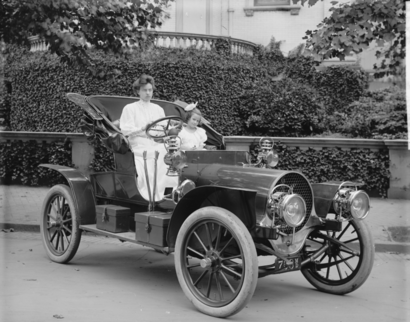
\includegraphics[width=\linewidth]{sample-franklin}
  \caption{1907 Franklin Model D roadster. Photograph by Harris \&
    Ewing, Inc. [Public domain], via Wikimedia
    Commons. (\url{https://goo.gl/VLCRBB}).}
  \Description{A woman and a girl in white dresses sit in an open car.}
\end{figure}

Your figures should contain a caption which describes the figure to
the reader.

Figure captions are placed {\itshape below} the figure.

Every figure should also have a figure description unless it is purely
decorative. These descriptions convey what’s in the image to someone
who cannot see it. They are also used by search engine crawlers for
indexing images, and when images cannot be loaded.

A figure description must be unformatted plain text less than 2000
characters long (including spaces).  {\bfseries Figure descriptions
  should not repeat the figure caption – their purpose is to capture
  important information that is not already provided in the caption or
  the main text of the paper.} For figures that convey important and
complex new information, a short text description may not be
adequate. More complex alternative descriptions can be placed in an
appendix and referenced in a short figure description. For example,
provide a data table capturing the information in a bar chart, or a
structured list representing a graph.  For additional information
regarding how best to write figure descriptions and why doing this is
so important, please see
\url{https://www.acm.org/publications/taps/describing-figures/}.

\subsection{The ``Teaser Figure''}

A ``teaser figure'' is an image, or set of images in one figure, that
are placed after all author and affiliation information, and before
the body of the article, spanning the page. If you wish to have such a
figure in your article, place the command immediately before the
\verb|\maketitle| command:
\begin{verbatim}
  \begin{teaserfigure}
 \includegraphics[width=\textwidth]{sampleteaser}
    \caption{figure caption}
    \Description{figure description}
  \end{teaserfigure}
\end{verbatim}

\section{Citations and Bibliographies}

The use of \BibTeX\ for the preparation and formatting of one's
references is strongly recommended. Authors' names should be complete
--- use full first names (``Donald E. Knuth'') not initials
(``D. E. Knuth'') --- and the salient identifying features of a
reference should be included: title, year, volume, number, pages,
article DOI, etc.

The bibliography is included in your source document with these two
commands, placed just before the \verb|\end{document}| command:
\begin{verbatim}
  \bibliographystyle{ACM-Reference-Format}
  \bibliography{bibfile}
\end{verbatim}
where ``\verb|bibfile|'' is the name, without the ``\verb|.bib|''
suffix, of the \BibTeX\ file.

Citations and references are numbered by default. A small number of
ACM publications have citations and references formatted in the
``author year'' style; for these exceptions, please include this
command in the {\bfseries preamble} (before the command
``\verb|\begin{document}|'') of your \LaTeX\ source:
\begin{verbatim}
  \citestyle{acmauthoryear}
\end{verbatim}


  Some examples.  A paginated journal article \cite{Abril07}, an
  enumerated journal article \cite{Cohen07}, a reference to an entire
  issue \cite{JCohen96}, a monograph (whole book) \cite{Kosiur01}, a
  monograph/whole book in a series (see 2a in spec. document)
  \cite{Harel79}, a divisible-book such as an anthology or compilation
  \cite{Editor00} followed by the same example, however we only output
  the series if the volume number is given \cite{Editor00a} (so
  Editor00a's series should NOT be present since it has no vol. no.),
  a chapter in a divisible book \cite{Spector90}, a chapter in a
  divisible book in a series \cite{Douglass98}, a multi-volume work as
  book \cite{Knuth97}, a couple of articles in a proceedings (of a
  conference, symposium, workshop for example) (paginated proceedings
  article) \cite{Andler79, Hagerup1993}, a proceedings article with
  all possible elements \cite{Smith10}, an example of an enumerated
  proceedings article \cite{VanGundy07}, an informally published work
  \cite{Harel78}, a couple of preprints \cite{Bornmann2019,
    AnzarootPBM14}, a doctoral dissertation \cite{Clarkson85}, a
  master's thesis: \cite{anisi03}, an online document / world wide web
  resource \cite{Thornburg01, Ablamowicz07, Poker06}, a video game
  (Case 1) \cite{Obama08} and (Case 2) \cite{Novak03} and \cite{Lee05}
  and (Case 3) a patent \cite{JoeScientist001}, work accepted for
  publication \cite{rous08}, 'YYYYb'-test for prolific author
  \cite{SaeediMEJ10} and \cite{SaeediJETC10}. Other cites might
  contain 'duplicate' DOI and URLs (some SIAM articles)
  \cite{Kirschmer:2010:AEI:1958016.1958018}. Boris / Barbara Beeton:
  multi-volume works as books \cite{MR781536} and \cite{MR781537}. A
  presentation~\cite{Reiser2014}. An article under
  review~\cite{Baggett2025}. A
  couple of citations with DOIs:
  \cite{2004:ITE:1009386.1010128,Kirschmer:2010:AEI:1958016.1958018}. Online
  citations: \cite{TUGInstmem, Thornburg01, CTANacmart}.
  Artifacts: \cite{R} and \cite{UMassCitations}.

\section{Acknowledgments}

Identification of funding sources and other support, and thanks to
individuals and groups that assisted in the research and the
preparation of the work should be included in an acknowledgment
section, which is placed just before the reference section in your
document.

This section has a special environment:
\begin{verbatim}
  \begin{acks}
  ...
  \end{acks}
\end{verbatim}
so that the information contained therein can be more easily collected
during the article metadata extraction phase, and to ensure
consistency in the spelling of the section heading.

Authors should not prepare this section as a numbered or unnumbered {\verb|\section|}; please use the ``{\verb|acks|}'' environment.

\section{Appendices}

If your work needs an appendix, add it before the
``\verb|\end{document}|'' command at the conclusion of your source
document.

Start the appendix with the ``\verb|appendix|'' command:
\begin{verbatim}
  \appendix
\end{verbatim}
and note that in the appendix, sections are lettered, not
numbered. This document has two appendices, demonstrating the section
and subsection identification method.

\section{Multi-language papers}

Papers may be written in languages other than English or include
titles, subtitles, keywords and abstracts in different languages (as a
rule, a paper in a language other than English should include an
English title and an English abstract).  Use \verb|language=...| for
every language used in the paper.  The last language indicated is the
main language of the paper.  For example, a French paper with
additional titles and abstracts in English and German may start with
the following command
\begin{verbatim}
\documentclass[sigconf, language=english, language=german,
               language=french]{acmart}
\end{verbatim}

The title, subtitle, keywords and abstract will be typeset in the main
language of the paper.  The commands \verb|\translatedXXX|, \verb|XXX|
begin title, subtitle and keywords, can be used to set these elements
in the other languages.  The environment \verb|translatedabstract| is
used to set the translation of the abstract.  These commands and
environment have a mandatory first argument: the language of the
second argument.  See \verb|sample-sigconf-i13n.tex| file for examples
of their usage.

%%
%% The acknowledgments section is defined using the "acks" environment
%% (and NOT an unnumbered section). This ensures the proper
%% identification of the section in the article metadata, and the
%% consistent spelling of the heading.
\begin{acks}
To Robert, for the bagels and explaining CMYK and color spaces.
\end{acks}


\section*{Ethics and Privacy Statement}

This section of your ACM work should discuss the potential societal
risks that might result from its publication; two to three sentences
related to the findings of your study, or new advancements made
possible by their developed methods. The privacy and ethics statement
should clearly address the broader impacts of their work as it relates
to the authors' interpretation of privacy, fairness, safety, human
rights, data sovereignty, or future misuse and any benefit/risk
trade-off resulting from this research. We acknowledge that some
papers may have minimal societal risks beyond those considered by
institutional review boards, and the dimensions considered by any
review of the user study design or dataset licenses could be provided
in this statement.

%%
%% The next two lines define the bibliography style to be used, and
%% the bibliography file.
\bibliographystyle{ACM-Reference-Format}
\bibliography{sample-base}


%%
%% If your work has an appendix, this is the place to put it.
\appendix

\section{Research Methods}

\subsection{Part One}

Lorem ipsum dolor sit amet, consectetur adipiscing elit. Morbi
malesuada, quam in pulvinar varius, metus nunc fermentum urna, id
sollicitudin purus odio sit amet enim. Aliquam ullamcorper eu ipsum
vel mollis. Curabitur quis dictum nisl. Phasellus vel semper risus, et
lacinia dolor. Integer ultricies commodo sem nec semper.

\subsection{Part Two}

Etiam commodo feugiat nisl pulvinar pellentesque. Etiam auctor sodales
ligula, non varius nibh pulvinar semper. Suspendisse nec lectus non
ipsum convallis congue hendrerit vitae sapien. Donec at laoreet
eros. Vivamus non purus placerat, scelerisque diam eu, cursus
ante. Etiam aliquam tortor auctor efficitur mattis.

\section{Online Resources}

Nam id fermentum dui. Suspendisse sagittis tortor a nulla mollis, in
pulvinar ex pretium. Sed interdum orci quis metus euismod, et sagittis
enim maximus. Vestibulum gravida massa ut felis suscipit
congue. Quisque mattis elit a risus ultrices commodo venenatis eget
dui. Etiam sagittis eleifend elementum.

Nam interdum magna at lectus dignissim, ac dignissim lorem
rhoncus. Maecenas eu arcu ac neque placerat aliquam. Nunc pulvinar
massa et mattis lacinia.

\end{document}
\endinput
%%
%% End of file `acmmanuscript.tex'.
